\documentclass[upright, contnum]{umemoria}

\usepackage[lined,ruled]{algorithm2e}
\usepackage{booktabs}
\usepackage{graphicx}
\usepackage{subcaption}
\usepackage{tikz}
\usetikzlibrary{shapes}

% allow full width tables
\usepackage{tabularx}

\usepackage{multirow}



%fix for the oneside argument
\makeatletter
\g@addto@macro\titlepage{\pagenumbering{Alph}}
\g@addto@macro\endtitlepage{\pagenumbering{roman}}
\makeatother

\depto{Departamento de Ciencias de la Computación}
\author{Mauricio Daniel Quezada Veas}
\title{KNOWLEDGE DISCOVERY FROM NEWS EVENTS ON TWITTER}
\auspicio{\break CONICYT PCHA/Doctorado Nacional 2015/21151445}
\date{Marzo 2019}
\guia{BÁRBARA POBLETE}
\carrera{Doctor en Ciencias, Mención Computación}
\memoria{Tesis para optar al Grado de \break  Doctor en Ciencias, Mención Computación}
\comision{AIDAN HOGAN \break MARCELO MENDOZA \break BRIAN D. DAVISON}

\usepackage{lipsum}

\usepackage[utf8]{inputenc}
\usepackage[T1]{fontenc}
 
\begin{document}

\frontmatter
\maketitle 

\begin{abstract} 
    Online activity involves the consumption and production of event-related content. On Twitter, about 500 million
    messages are published every day, and according to surveys, 59\% 
    of its users use the platform as a way to get the
    news. The high rate of production of multimodal content (text, images, and videos) makes it a necessity to have flexible
    models to understand the dynamics of the information disseminated on social media. This thesis proposes the creation of
    context models from user-generated messages on Twitter to discover knowledge as a way to perform high-level quantitative
    analysis of news events. These models are meant to be useful in three perspectives: the spatio-temporal context in which
    the events develop, the activity of users that react when a high-impact event happens, and the multimodal content that can
    be exploited to generate a comprehensive summary of the event. Our current work involves the creation of a geopolitical
    model that relates events and countries, allowing us to discover international relations; the study of what features make an
    event susceptible to provoke high activity from users, and a characterization that allows us to predict with high precision
    which events are going to produce high activity; and our ongoing work on generating automatic multimodal summaries of
    events based on the assumption that the users describe the non-textual content in their tweets when they manifest their
    facts and opinions around events.
\end{abstract}

\begin{dedicatoria} % opcional
Una dedicatoria corta. Por ejemplo, al \emph{Centro Tecnológico Ucampus}
\end{dedicatoria}

\begin{thanks} % opcional
\lipsum[1-2]
\end{thanks}
\cleardoublepage

\tableofcontents
\listoftables % opcional
\listoffigures % opcional

\mainmatter

\chapter{Introduction}

% WHAT IS SOCIAL MEDIA

The so-called {\em Web 2.0} represents a change in how users interact with the
Web.
%
Currently, the Web acts as a system that encourages end-users to publish and
consume content. 
%
One of the main manifestations of this phenomena are {\em online social
networks}.
%
Users make connections with other users online based on different criteria, and
start to produce content.
%
Social platforms such as Facebook~\cite{facebook}, Twitter~\cite{twitter},
or Sina Weibo~\cite{weibo} are now among the most used ways to connect with
family, friends, acquaintances, co-workers, or strangers with similar interests.
%
Users interact with each other and produce or share content about their lives,
thoughts, or what is happening around the world, etc.    
%
This collective of information published in these Internet-based applications,
such as microblogging platforms, blogs, wikis, etc., is called {\em
social media}~\cite{kaplan2010users}.

%%
% CONTENT IN SM

Content in social media is multimodal. 
%
Twitter, for example, encourages users to publish short texts (initially limited
to 140 characters, now 280), but it recently started to promote that users share
more photographs~\cite{brown_2019}.
%  
And with the proliferation of smartphones and internet-connected devices, more
of this information is also geo-tagged and in ``real-time''. 
%
For instance, Foursquare~\cite{foursquare} is an application for smartphone
users to tag and comment about locations around the world, which became a
repository of data about businesses and points of interest.
%
Whether via text, images, videos, sounds or hyperlinks, social media lowered the
entry barriers for content producers and made it easy for consumers to access a
myriad of different pieces of information.


%%


% UTILITY, APPLICATIONS OF SM

The influence of social media on today's society cannot be denied, as it
facilitates co\-mmu\-nication among people and speeds up the diffusion of
information. 
%
For instance, it is believed that the revolutionary wave of protests and
uprisings in the Arab states (known as the Arab Spring, which began in 2010) was
highly influenced by social media as a means of organizing and facilitating
communication~\cite{howard2011opening}. 
%
Also, it has permitted many applications to proliferate in emergency management
and detection, such as earthquake alert systems using
Twitter~\cite{Sakaki2010,Sakaki:Tweet:2013,Sarmiento:2018:DDE:3201064.3201077,Mendoza2019}.
%
The usefulness of quantitative analysis of events through time is undeniable, and
social media offers a window to see and capture information about those events,
how they develop, and how the world interprets them.\\

%%% DEFINITION OF EVENT:
We define an {\bf event} as a conglomerate of information that encompasses all
of the social media content related to a real-world news occurrence. 
%
We will use this specification throughout this work, which considers an event as
a complex unit of information, in contrast to other interpretations, such as
those that consider an event as represented by a single unit or piece of
information, like a news article, a video, or a structured and pre-defined
description.

% NEWS CONSUMPTION AND PRODUCTION
One of the main uses of social media platforms is the consumption and generation
of real-world event-related content. 
%
According to a recent 2018 study~\cite{pewresearch}, about two thirds of adults
in the U.S. obtain their news from social media.
%
The most used platforms for news are Facebook, YouTube, and Twitter, with the
latter having over 70\% of its users using the platform to consume news.
%
Furthermore, almost every news outlet has a presence in social media
in order to attract readers and viewers.
%
In this way, users comment on the news events, reacting to them according to a
myriad of factors, and many of these characteristics are present in one way or
another in social media.
%
Therefore, we see social media as a medium that reflects an important 
part of what society thinks about what is happening in the world.




% PROBLEMS

However, the popularity of social media is not without issues. 
%
{\em Information overload} refers to the problem of being unable to manage or to
make decisions based on data, due to the high volume of information available
and the limited capabilities of the person who is dealing with it. 
%
Humans have limited cognitive processing capacities, and when they are
overloaded with information, their quality of decision making
suffers~\cite{gross1964managing}. 
%
In the context of social media, the high availability of diverse information may
prevent users from finding relevant content.

%%

Finding relevant content in social media is not easily solved by conventional
search engines.
%
Social media publications, or {\em posts}, can be of {\em variable quality}.
%
Posts are composed of multimedia pieces of content, but often they are brief.
%
For instance, a post can be a very short text, an hyperlink, a single image or
video with little context.
%
They can be also irrelevant to the interest of a particular user, for example,
spam posts, which are posts that contain relevant keywords but in a misleading way, in
order to lure users to irrelevant websites. 
%
Posts can also be out-dated, delivering incorrect or obsolete information. 
%
Many posts can be duplicates, published by automated agents, or by users
using ``share buttons'' in websites publishing posts with a template text; 
%
they can also be near-duplicates, with minor text differences, or sharing the
same resource from different URLs.
%
Another important characteristic of posts is that they are written in natural
language, so they can be incorrectly capitalized, misspelled, or with ambiguous
meaning.
%
Users make use of colloquial language and different forms of expression when
publishing content, e.g., abbreviations, hashtags (tags to describe content),
emojis (ideograms), etc.
%
Finally, messages can also be misleading, sharing false information.
%
All of these particularities of social media make it difficult to apply standard
techniques for users to find relevant content.

%%

At the same time, there is a massive scale of content production.
%
Twitter reports that there are about 320 million monthly active users and 500
million {\em tweets} daily\footnote{These numbers were first stated in 2014 and
have not been updated since then.}, i.e., messages published in their
platform~\cite{twitter2014}. 
%
Facebook has nearly 2.32 billion monthly active users~\cite{fbnewsroom}. 
%
Sina Weibo has 462 million monthly active users, where 93\% of them are on
mobile devices~\cite{chinawatch}.
%
The amount of content being published requires novel ways to deal with social
media data, in particular, news events.


%%

%We define a news event as a higher-level abstraction composed of individual
%posts about a real-world occurrence.\todo[inline]{mejor sacar esta frase se repite despues}
%
In related work, an event\footnote{In this work, we will use the term {\em news
event} and {\em event} interchangeably.} is deemed as {\em something that happens
in a certain place and time}~\cite{yang1999learning}, while other definitions
consider an event as a collection of documents related to a certain
occurrence~\cite{Becker:2010:LSM:1718487.1718524}.
%
Throughout this thesis, we will consider an event as a collection of
social media posts describing or commenting on a real-world occurrence.
%
In this sense, an event is a more complex piece of information compared to
single posts.
%
This notion of event is useful as it is the base unit for new tasks, such as
event detection, tracking, or summarization.
%
Also, an event is comprised of posts of heterogeneous quality, from different
locations, and at different times.
%
This yields new problems and challenges when studying social media.

%%

% PROPOSAL

\section{Objectives}

In this thesis we tackle the problem of {\em extracting useful
knowledge} from events on social media. 
%
To be able to infer and extract useful information from events, we propose the
creation of event representations that leverage specific features according
to the desired goal when analyzing social media data.
%
For this, we propose different models or representations of events based on
three perspectives:
%

\begin{enumerate}
    \item {\bf User activity.} 
    %
    When users react to an event, they may manifest this reaction on social
    media, producing or sharing content relevant to the event. 
    %
    The characteristics of these manifestations are dependent on the particular
    features of the occurrence, and not all are equal. 
    %
    We look at how the activity of users offers insight on the specific
    features of an event and incorporates this behavior in a compact
    representation.

    \item {\bf Spatio-temporal context.} 
    %
    Events occur in different locations. 
    %
    On the other hand, users from different locations may react differently to
    the same event.
    % 
    We study the evolution of events based on user activity conditioned by the
    location users are from, proposing a representation of events and locations
    based on social media posts.

    \item {\bf Content.} 
    %
    Users may publish similar pieces of content in social media in reaction to
    events.
    %
    However, each post can contribute to a different aspect of the event, while
    sharing some common features.
    %
    We leverage these commonalities in content in order to produce a compact model that
    preserves topical information in events.
    
\end{enumerate}


% OBJETIVES

Our main objective is to define event representations through different data
aggregations in order to perform quantitative analysis of news events on social media.
%
Currently, it is very difficult to manage and analyze the high volume of
information being published when an event occurs. 
%
In particular, we study events through three perspectives: user reaction
and activity, spatio-temporal context of events, and content aggregation.
%
Understanding user reaction involves discriminating which events are more
important or produce more impact in a community. 
%
Analyzing spatio-temporal context refers to understanding how communities from
different locations are affected by different events, as seen on social media,
and identifying similar communities and events based on this context. 
%
Understanding content refers to the identification of the core aspects of an
event, without having to go through all the --potentially many-- posts.
%
In particular, our goal is to propose different models for representing events. 
%
These models should be flexible enough to apply diverse methodologies to
discover useful knowledge from information published on social media about
real-world events, from the perspectives described above. 


%%

% WHY TWITTER
\section{Why Twitter?} 

We chose Twitter as our data source for this work. 
%
The majority of Twitter posts are, in general, public, and data can be obtained
in a simple way automatically via its API (Application Programming
Interface~\cite{twitterapi}).
%
Furthermore, it is not as restrictive as other platforms, such as Facebook,
in which users maintain a private profile.
%
Also, Facebook encourages users to share more personal content, and not just
event-related.
%
Twitter, on the other hand, is primarily dedicated to share event-related posts,
and it is mostly utilized as a news source by about 70\% of its users. 
%
For instance, its website asks ``What's happening?'' to users when publishing
content, as opposed to Facebook's ``What's on your mind?''


% UTILITY
\section{Applications}

The study of news event dissemination in online social networks has several
applications in the proposed setting. 
%
How the community reacts to different real-world phenomena can allow us to
characterize those events,
%
for example, by measuring user reaction, other social network features, or
analyzing event content.
%
Using these characteristics, we would be able to identify or even predict which
events are going to cause a significant reaction from the community, hence
improving journalistic coverage or providing better response from authorities in
face of an emergency.
%
Additionally, by studying not only the response, but the context of different
communities and how they respond to certain events, we may gain insights about
the communities themselves, for example, by revealing unexpected relations
between different communities, or by measuring event similarity using the
context, instead of content-based features. 
%
On the other hand, the study of the content is useful to understand the
different points of view ahead of an event. 
%
Users accustomed to the same perspectives given by other users or sources may be
oblivious of other information angles of the same news event. 
%
Being capable of identifying different aspects that compose an event and then
presenting these aspects in a concise summary can deal with this problem. 
%
All in all, the proposed framework can be of utility to understand social
behavior, study and decrease the effects of the information overload as well
as to perform comparative historical research~\cite{wiki:comparative}.

%%

\section{Thesis statement} 
%
This dissertation defines flexible models for events on the social
networking platform Twitter. 
%
Having three perspectives in mind: user reaction, spatio-temporal context, and
content, the defined models should be able to allow us to achieve new insights
about real-world events as seen by Twitter users. 
%
In particular, each perspective approaches a specific Data Mining and Information
Retrieval technique: 
%
the study of context involves modeling and exploratory data analysis; 
%
reaction analysis involves filtering and classification;
%
content involves topic detection and document modeling.
%
The proposed models are designed to be general and easily adaptable to other
online social networks.

The thesis statement is as follows:

% version corregida por barb:

\begin{tcolorbox}
        {\bf 
        Novel and effective forms of high-level analysis of news events can be
        achieved by using models that integrate information from user publications in
        online social networks, based on their spatio-temporal context, as well as the
        reaction that users had to the event itself, including multimedia content shared
        for the event.
        }
\end{tcolorbox}

% {\bf \em
% Modeling news events from user-contributed content on Twitter, based on
% their spatio-temporal context, the reaction the users had on them, or the
% multimedia content which the events contain, is novel and effective for performing
% high-level quantitative analyses of news events.
% }

% Statement of purpose

%\todo[inline]{statement of purpose}


\section{Challenges} 

We identify three main challenges for this work:

\begin{itemize}
    \item {\bf Retrieval of relevant social media posts.} 
    Mainstream topics obfuscate distinct points of view, which can
    obstruct retrieval of diverse and relevant content to an event. 
    %
    Here, relevance to a topic is defined as the similarity between a piece of
    content and the topic which this piece refers to.
    %
    Because users are frequently posting messages about their own lives, daily
    situations, or general topics, trends can only be visible when looking at large
    volumes of data. 
    %
    This makes identification of events and relevant content a very difficult task.
    %
    Due to the characteristics of Twitter (or any other online social network),
    messages are usually very short and noisy.
    %
    Users spontaneously create new ways to refer to the same entities
    (e.g., via the use of hashtags, emojis, or abbreviations), making it
    difficult to identify more relevant content when detecting events.
    %
    Relevant multimedia content is also difficult to identify. 
    %
    Multimedia content is represented by images, videos, text, or a mix of them,
    etc. 
    %
    This information can be exploited to improve the effectiveness of
    the proposed methodologies. 
    %
    The challenge consists of how to identify such content in an efficient way,
    how to deal with duplicated or quasi-duplicated content, and how to evaluate
    the effectiveness of methodologies when presenting multimedia content. 

    \item {\bf Bias in the collected data.}
    Social media offers a partial view of the world. 
    %
    Furthermore, the employed methodologies to retrieve or identify events from
    social media may be biased depending on several factors. 
    %
    For instance, we collected our dataset using news outlets as sources, with
    the majority of outlets coming from the USA or the UK. 
    %
    Our sources also use specific words and ways to express the information,
    which can also create a bias in the way we further retrieve more tweets.
    %
    This is a huge challenge in order to provide generalizable results from the
    proposed methodologies. 
    %
    In addition, it is challenging to ensure that our results are as diverse as
    the data source. 

    \item {\bf Validation of results.} 
    As data in social media is being published at all times, it is unfeasible to
    apply standard measures such as Recall when evaluating a methodology,
    because we do not have all the relevant content available.
    %
    On the other hand, there are no {\em gold standards} to which we can
    contrast our models. 
    %
    We need to come up with methodologies to validate our results in order to
    provide generalizable results.
    
\end{itemize}


\paragraph{A note on the veracity of the data.} 
%
Misinformation, fabricated content, and automated tools to publish content at
large scale correspond to an important challenge when analyzing social media
information.
%
In this work we apply simple measures to avoid some forms of non-relevant
content, such as the removal of messages that share several URLs at the same
time, hashtags, etc.
%
We also make the assumption that the events we collected (see
Chapter~\ref{chapter:data}) correspond to real-world occurrences reported by
verified and recognized news outlets.
%
The identification and characterization of misleading information is an active
line of research at the time of this dissertation, but we do not apply more
sophisticated techniques to tackle this potential issue.
%
We discuss further this issue when discussing the bias in our data in
Section~\ref{sec:geo:mining} and in Chapter~\ref{sec:conclusions}.



\section{Contributions} 

This thesis presents four main contributions, as follows:

\begin{enumerate}
    \setlength\itemsep{0.5em}

\item A novel representation of event information based on user activity
triggered by real-world events in Twitter (Chapter~\ref{chapter:high-activity}).
%
This representation allows us to rank events into different levels of user
activity. 
%
We also show that the activity can be determined by other event features, and
that these features appear early during event evolution.
%
We show that it is possible to {\em predict} early on the level of activity that
an event will produce using aggregated features.

\item A spatio-temporal representation based on the location where an event
takes place, and the locations from where users are commenting about the news
(Chapter~\ref{chapter:geopolitical}).
%
With this type of representation, we can compare events and locations based on
different factors, and track the evolution of an event based on the locations
involved in it.

\item A lightweight representation of content based on shared URLs
(Chapter~\ref{chapter:url}).
%
This representation consists of aggregation of user posts based on common URLs,
retweets, and replies. 
%
In our preliminary experiments, we observe that the representation is one order
of magnitude smaller than the original data.
%
At the same time, we observe that with our representation we can achieve
comparable clustering results, with a fraction of running time and memory
required.

\item An event collection methodology based on {\em seed news outlets}
(Chapter~\ref{chapter:data}).
%
Given a set of news outlets, every hour we extract the most relevant keywords
from their headlines and use them to retrieve relevant tweets from regular
users.
%
We also made available a dataset of 193 million tweets of $20,000$ news events,
from 2013 to 2015.
\end{enumerate}

Even though the different points of view posed as themes for this project cover
mostly independent approaches of event mining, they have in common the goal of
exploring and studying how different data aggregations can be useful for
extracting useful knowledge from events. 
%
This dissertation can be viewed as an exploration on how different data
aggregation strategies applied to events on social media are useful for easily
extracting knowledge or to serve as building blocks for new models and
methodologies.


\newpage

\section*{Publications} 

The following publications are associated with this dissertation:

{\bf Journal papers.}
\begin{itemize}
    \setlength\itemsep{1em}

    \item J. Kalyanam, {\bf M. Quezada}, B. Poblete, and G. Lanckriet. {\em
     Prediction and Characterization of High-Activity Events in Social Media
     Triggered by Real-World News}. In PLOS ONE 11(12): e0166694. 2016.

    \item V. Peña-Araya, {\bf M. Quezada}, B. Poblete, and D. Parra. {\em
    Gaining historical and international relations insights from social media:
    spatio-temporal real-world news analysis using Twitter.} In EPJ Data Science
    6, no. 1 (2017): 25. 2017.
\end{itemize}

\vspace{1em}

{\bf Conference and Workshop papers.}

\begin{itemize}
    \setlength\itemsep{1em}

    \item {\bf M. Quezada}, V. Peña-Araya, and B. Poblete. {\em Location-Aware
    Model for News Events in Social Media.} In Proceedings of the 38th
    International ACM SIGIR Conference on Research and Development in
    Information Retrieval (SIGIR '15). ACM, New York, NY, USA. 2015.
    (Short paper.)

    \item V. Peña-Araya, {\bf M. Quezada}, and B. Poblete. {\em Galean:
    Visualization of Geolocated News Events from Social Media.} In Proceedings
    of the 38th International ACM SIGIR Conference on Research and Development
    in Information Retrieval (SIGIR '15). ACM, New York, NY, USA. 2015.
    (Demo paper.)

    \item {\bf M. Quezada} and B. Poblete. {\em A Lightweight Representation of
    News Events on Social Media.} In Proceedings of the 42nd International ACM
    SIGIR Conference on Research and Development in Information Retrieval (SIGIR
    '19). (Short paper.)

    \item {\bf M. Quezada.} {\em Knowledge Discovery of News Events in Social
    Media.} Published within the CEUR-WS workshop proceedings, in the 9th
    PhD Symposium on Future Directions in Information Access (FDIA '19). 

\end{itemize}

%%


\chapter{State of the Art}


\section{Event Models in Social Media}

\section{Quantitative Analysis of News Events}

\chapter{Data Collection Methodology}
\label{chapter:data}  


We use the Twitter Application Programming Interface~\cite{twitterapi}, or also
{\em Twitter API}, to retrieve tweets from Twitter. 
%
Our methodology consists in gathering tweets and then identifying coherent
events. 
%
Our dataset consists of 20,066 news events. These events encompass 193,445,734
tweets, produced by 26,127,624 different users.

%%

Section~\ref{sec:dataset} describes the steps to follow to build the dataset,
while Section~\ref{sec:cleaning} describes data cleaning and validation.


\section{Building the Dataset}\label{sec:dataset}

The dataset was constructed using a set of seed Twitter accounts, from which
newsworthy messages were obtained.
%
From these messages, we identified relevant keywords which describe the current
event, and used them to retrieve tweets from the general public to improve
recall.
%
Finally, we grouped some of these sets into {\em events}.


% \begin{enumerate}
% \item \textbf{Tweet}: A social media object consisting of a text message with
%   metadata: author's data (name, followers, followees, etc.), date of
%   publication (timestamp), number of times it was \emph{retweeted} or re-shared,
%   etc.

% \item \textbf{Search Result}: A search result is a tuple consisting of a pair of
%   keywords and a date that represents it, and a set of tweets associated with
%   it, as every tweet message in the set contains both keywords.

% \item \textbf{Event}: An event is going to be considered as an extended version
%   of a search result. In other words, it is a tuple consisting of a set of
%   keywords, a date and a set of tweets. Each tweet message contains at least two
%   keywords of the keywords set. For example, Figure~\ref{fig:event-example}
%   shows an event consisting of three searches. An event is produced by joining
%   keywords from the search results, as described in Section~\ref{subsec:group}.
% \end{enumerate}

\subsection{Collecting related posts for news on Twitter}

The Twitter API~\cite{twitterapi} provides an interface to retrieve tweets in an
automated manner. For building a dataset of news events, it is necessary to
somehow identify events from the Twitter stream.

Essentially, there are two ways to retrieve tweets from Twitter: using the
{\em Streaming API}, or the {\em REST API}. 
%
The Streaming API provides a way to retrieve real time tweets using zero or more
keywords to filter the stream. 
%
The amount of tweets that we can obtain is capped up to 1\% of the real stream
at a given moment\footnote{The \emph{firehose} or full stream corresponds to the
full stream of tweets. The Streaming API samples up to 1\% of those tweets that
come every second. However, there was evidence that the Streaming API is not a
good random sample in some cases, for example, when looking for the top hashtags
in a period of time~\cite{morstatter2013sample}.}.  
%
The REST API allows us to get tweets from the past\footnote{However, the
documentation is not clear in terms of how long nor how many tweets can be
retrieved.}, by giving it a search term, consisting on one or more keywords. 
%
Both services return a set of tweets after a period of time. 

As our initial motivation was to study the characteristics of a news event when
it breaks, we wanted to obtain as many tweets as possible from that moment.
%
For that reason, it was necessary to get tweets about events event before they
were reported\footnote{Tweets related to the topic. For example, tweets about
Nelson Mandela before his death.}, and after that, to see the change in volume.
%
With this in mind, we chose to use the REST API.

We manually crafted a set of about fifty verified news accounts in Twitter (such
as BBCNews, CNN, Al Jazeera, etc.). 
%
The full list of news sources can be found in Appendix~\ref{ape:news}.
%
Most of the news accounts are from the United States, or English spoken.
%
The list was made manually by performing a search for ``news'' in the Twitter
site\footnote{\url{https://twitter.com/search?q=news&src=typd&mode=users}} and
selecting verified users. 
%
Verified accounts are accounts that were verified for identity
authenticity\footnote{\url{https://support.twitter.com/articles/119135-faqs-about-verified-accounts}},
although how the process of verification is made is unknown outside Twitter. 

Each of these accounts posts messages about news, some of them breaking, and
sometimes they post advertising, etc. 
%
Let the tweets posted from those accounts be called \emph{headlines}. Some
examples of headlines are the following: 

{\it 
\begin{itemize}
\item @BBCNews: RT @BBCSport: FT: Uruguay 2-1 England. Two goals from
  Luis Suarez enough to beat \#ENG. <URL> \#WorldCup
  \#ENGvsURU <URL>…
\item @BreakingNews: Presbyterian General Assembly votes to allow
  pastors to preside at same-sex marriages - @AP
  <URL>
\item @Channel4News: Chile mountain top is blown off - in the name of
  astrophysics: <URL> \#c4news
\item @BBCNewsUS: Kevin McCarthy elected Republican House majority
  leader, party's second-ranking post <URL>
\end{itemize}
}

Our assumption is that if an important event is happening in a certain moment in
time, then several news accounts will be reporting on that event shortly after,
using similar vocabulary in their reporting.
%
From this assumption, we collected headlines every hour, identified the most
common keywords from the headlines, and used those keywords to search for more
tweets in the API.

\begin{figure}
\begin{center}
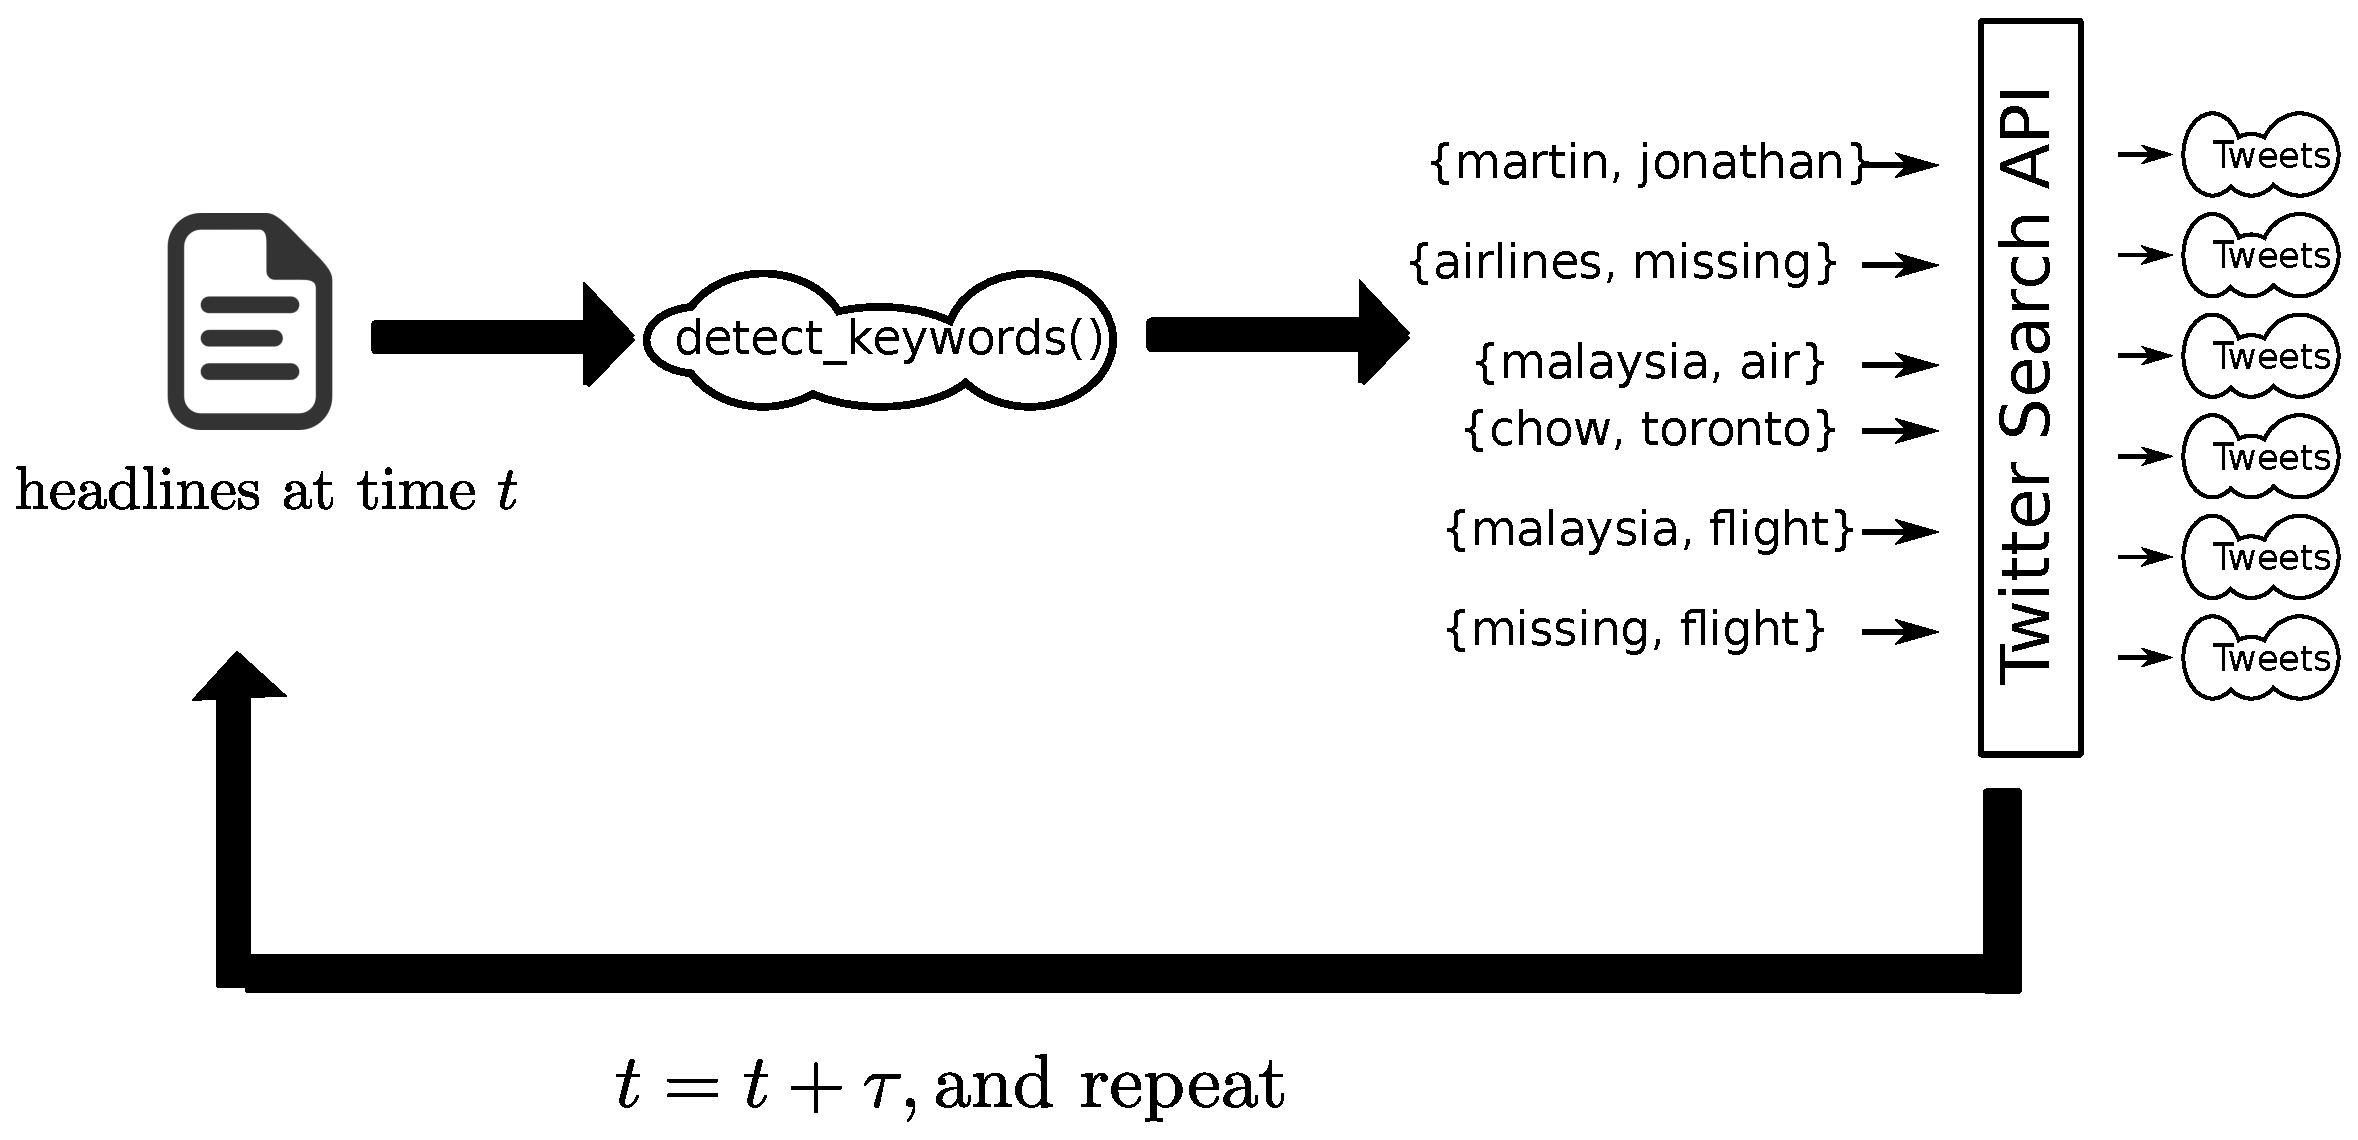
\includegraphics[width=\textwidth]{figures/data/data_collection_1}
\caption[Pipeline of data collection]{Pipeline of data collection. From the
  selected news accounts a set of headlines (tweets) are retrieved. Then, six
  pairs of keywords are identified based on the most frequent itemsets present
  in the headlines. Each pair of keywords is used as a search term of the
  Twitter REST API. For one hour, the process retrieves tweets related to each
  pair of keywords. After that, the process starts again for the next set of
  headlines.}
\label{fig:pipeline}
\end{center}
\end{figure}



Every $t=60$ minutes, all headlines posted in the last $t$ minutes are
retrieved using the API. 
%
We pre-process the retrieved headlines by removing stopwords, punctuation, URLs,
hashtags, mentions, and converting words to lowercase.
%
Then, from the processed headlines the most frequent sets of words are chosen.
%
From the resulting sets, the top $k=2$ words are chosen from each of the top
$g=6$ groups. 
%
Each pair of words, or keywords, are used as input for the REST API to retrieve
tweets related to the keywords. 
%
The main idea is that if several headlines discuss the same topic, then it is
considered an important topic, and users talk about it using some of the most
frequent words. 
%
The algorithm to identify the frequent itemsets~\cite{zaki2000scalable} is
described in Algorithm~\ref{alg:detect_keywords}.
%


\renewcommand{\algorithmicrequire}{\textbf{Input:}}
\renewcommand{\algorithmicensure}{\textbf{Output:}}
\newcommand{\I}{\mathcal{I}}
\renewcommand{\G}{\mathcal{G}}
\newcommand{\ess}{\mathcal{S}}

\begin{algorithm}
\caption{Detect common keywords from headlines}
\label{alg:detect_keywords}
\begin{algorithmic}[1]
\REQUIRE A set of $M$ sets of words, $\ess= \{H_1,H_2, \ldots, H_M\}$, positive integers $k, \eta$
\ENSURE $k$ sets of keywords, $G = (\I_1,\I_2,\ldots,\I_{k})$
\STATE $\I_i \leftarrow \emptyset$ for $i = 1,2, \ldots,k$ %\COMMENT{Initialize item sets to empty sets}
\STATE $score_i \leftarrow$ empty dictionary for $i = 1, 2, \ldots,k$ %\COMMENT{Initialize keyword set scores to $1$}
\STATE $i \leftarrow 1$
\FOR{every pair of headlines $\{H_a, H_b\} \in \ess$ such that $|H_a \cap H_b| \geq \eta$}
    \STATE $\G \leftarrow H_a \cap H_b$ \label{alg:line:intersect} %\COMMENT{$\G$ is the set of common words of $H_a$ and $H_b$}
    \STATE $j \leftarrow \operatorname{arg\,max}_j |\I_j \cap \G|$
    \IF{$|\I_j \cap \G| \geq \eta$}
        \STATE $\I_j \leftarrow \I_j \cap \G$
        \STATE $score_{j}[w] \leftarrow score_{j}[w] + 1$ for all $w \in \I_j$
    \ELSE
        \STATE $\I_i \leftarrow \G$
        \STATE $score_{i}[w] \leftarrow 1$ for all $w \in \I_i$
        \STATE $i \leftarrow i + 1$
    \ENDIF
\ENDFOR
\STATE $total\_score_i \leftarrow \sum_{w \in \I_i} score_{i}[w]$ for $i=1,2,\ldots,k$
\RETURN $G = (\I_i$ sorted by $total\_score_i)$

\end{algorithmic}
\end{algorithm}

We only considered the top two keywords from each group, that is, we only
considered pairs of keywords from the headlines. 
%
This is because we use Twitter as our data source, and the tweets can be very
short (140 characters at most at the time of the data collection). 
%
Also, we selected only the top six groups, to obtain an acceptable rate of news
events per time unit. 
%
If there are not enough tweets or groups, we only choose the keywords available
for that period of time.

After one run of the process, a set of $g=6$ \emph{search results} or sets of
tweets are created and stored. 
%
A search is a tuple consisting of a pair of keywords and a set of tweets, each
one of those tweets contains both keywords in its text.

The REST API allows us to get tweets from even before the corresponding headline
was published.
%
Then the search continues for about one hour, to get all the related tweets. 
%
If there is a high impact news event, then the users will be tweeting about it
frequently. 
%
For that reason, the search is perfomed no more than one hour from the
publication time of the headlines. 
%
Figure~\ref{fig:pipeline} portrays the tweets collection methodology.



\begin{table}
{\small
\begin{center}
\begin{tabular}{lll}
\toprule
 Keywords            &  Date       &  Sample Tweet                                                                                                                                                                                                                     \\
\midrule
 woody allen         &  2014-01-13  &  I love how Woody Allen didn't
 accept his award at the Golden\ldots{} \\
 egypt constitution  &  2014-01-18  &  Egypt passes new constitution\ldots{} \\
 king luther         &  2014-01-20  &  I added a video to a @YouTube
 playlist\ldots{} \\
 brazil world        &  2014-01-26  &  Sports: Hundreds protest against
 World Cup in Brazil: \ldots{} \\
 city chelsea        &  2014-02-15  &  RT@mcfcbuzztap: TEAMtalk FA Cup:
 Manchester City\ldots{} \\
 \bottomrule
\end{tabular}
\end{center}
} \caption[Example of searches.]{Example of searches. The first column
corresponds to the pair of keywords retrieved from the headlines. The second
column corresponds to the date of the search. The last column shows an excerpt
of a tweet in that set.}\label{table:searches}
\end{table}

In summary, the data collection methodology allows for the most recent tweets to
be found on a certain event, assuming that the selected news accounts
consistently post about those events. 
%
The dataset obtained in this phase corresponds to pairs of keywords related to
an event, and a set of tweets that contains the two keywords in its text.
%
Table~\ref{table:searches} shows a few examples of searches.


\subsection{Identifying Events}

In order to identify events, it is necessary to group similar pairs of keywords.
%
The next step is to identify events from the keywords. 
%
For example, the pairs of keywords \{obama, syria\}, \{russia, g8\}, and
\{russia, syria\} detected in the same day correspond to the same event (the G8
summit about Syria on
2013\footnote{\url{http://rt.com/news/syria-russia-assad-g8-876/}}). 
%
On the other hand, a sole pair of keywords could be not enough to identify an
event. 
%
For that reason, it is necessary to group pairs of keywords (and the
corresponding tweets) into larger sets to form coherent events. 


\begin{table}

\begin{center}
\begin{tabular}{lllll}
\toprule
  Keywords              &  Date and time     &     &  Keywords              &  Date and time     \\
\midrule
 bill aid              &  2014-04-02 00:00  &     &  quake chile           &  2014-04-02 03:00  \\
 island refinery       &  2014-04-02 00:00  &     &  earthquake magnitude  &  2014-04-02 03:00  \\
 congress ukraine      &  2014-04-02 00:00  &     &  chile tsunami         &  2014-04-02 03:00  \\
 earthquake struck     &  2014-04-02 01:00  &     &  iquique chile         &  2014-04-02 03:00  \\
 tsunami chile         &  2014-04-02 01:00  &     &  chile five            &  2014-04-02 05:00  \\
 magnitude earthquake  &  2014-04-02 01:00  &     &  earthquake magnitude  &  2014-04-02 04:00  \\
 tsunami chile         &  2014-04-02 01:00  &     &  chile earthquake      &  2014-04-02 05:00  \\
 watches tsunami       &  2014-04-02 01:00  &     &  gray primary          &  2014-04-02 05:00  \\
 chile tsunami         &  2014-04-02 02:00  &     &  warning tsunami       &  2014-04-02 05:00  \\
 earthquake tsunami    &  2014-04-02 02:00  &     &  earthquake chile      &  2014-04-02 04:00  \\
 tsunami chile         &  2014-04-02 02:00  &     &  hawaii advisory       &  2014-04-02 05:00  \\
\bottomrule
\end{tabular}
\end{center}
\caption[Example pairs of keywords from April 2nd, 2014.]{Some pairs of
  keywords from April 2nd, 2014. Several keywords are related to an
  earthquake and tsunami occurred on Iquique, Chile that day. (The
  times are in UTC.)}\label{table:example-pairs}
\end{table}


For example, in Table~\ref{table:example-pairs}, there are some of the keywords
detected on April 2nd, 2014. 
%
Several of them contain the word ``earthquake'', ``tsunami'' or ``chile''.
%
Indeed, on that day an earthquake struck and was followed by a tsunami on the
coast of Iquique and Arica, in Chile. 
%
The occurrence of several pairs of keywords related to the same event is a
consequence of the news accounts posting several headlines about that event, in
different times. 
%
The tweets about the event did not last one hour, but instead several. 
%
For that reason, it is necessary to group similar pairs of keywords to form
events.

In our pipeline, we identify events every 24 hours of keyword collection. 
%
Using more time results in having big components of unrelated events joined
together, as we saw empirically.


\begin{table}
\begin{center}
\begin{tabular}{rl}
\toprule
 Keywords  &  Event                                                                        \\
\midrule
       16  &  chile, northern, iquique, panama, fires, watches, coast, canceled, tsunami,  \\
           &  five, quake, following, struck, warning, earthquake, magnitude               \\
       11  &  europe, jobs, clegg, 191, tonight, nick, won, farage, nigel, farage, round   \\
        9  &  passengers, police, scene, four, incident, details, active, hood, fort       \\
        4  &  wall, prime, school, edinburgh                                               \\
        3  &  modi, narendra, buxar                                                        \\
        2  &  paul, cosford                                                                \\
        2  &  interior, ministry                                                           \\
        2  &  president, bachelet                                                          \\
        2  &  firetv, amazon                                                               \\
\bottomrule
\end{tabular}
\end{center}

\caption[Some events identified from April 2nd, 2014.]{Some events
  identified from April 2nd, 
  2014. The largest event corresponds to the earthquake in Chile. They
  are sorted on the number of keywords.}\label{table:example-events}
\end{table}

The approach is as follows: join two pairs of keywords if they share a common
word.
%
If each word is seen as a node in a graph, and a pair of keywords represents an
(undirected) edge, then the events are connected components of the graph (see
Figure~\ref{fig:connected-component}).
%
In Table~\ref{table:example-events} there are some events identified in April
2nd, 2014. 


\begin{figure}
    \centering
    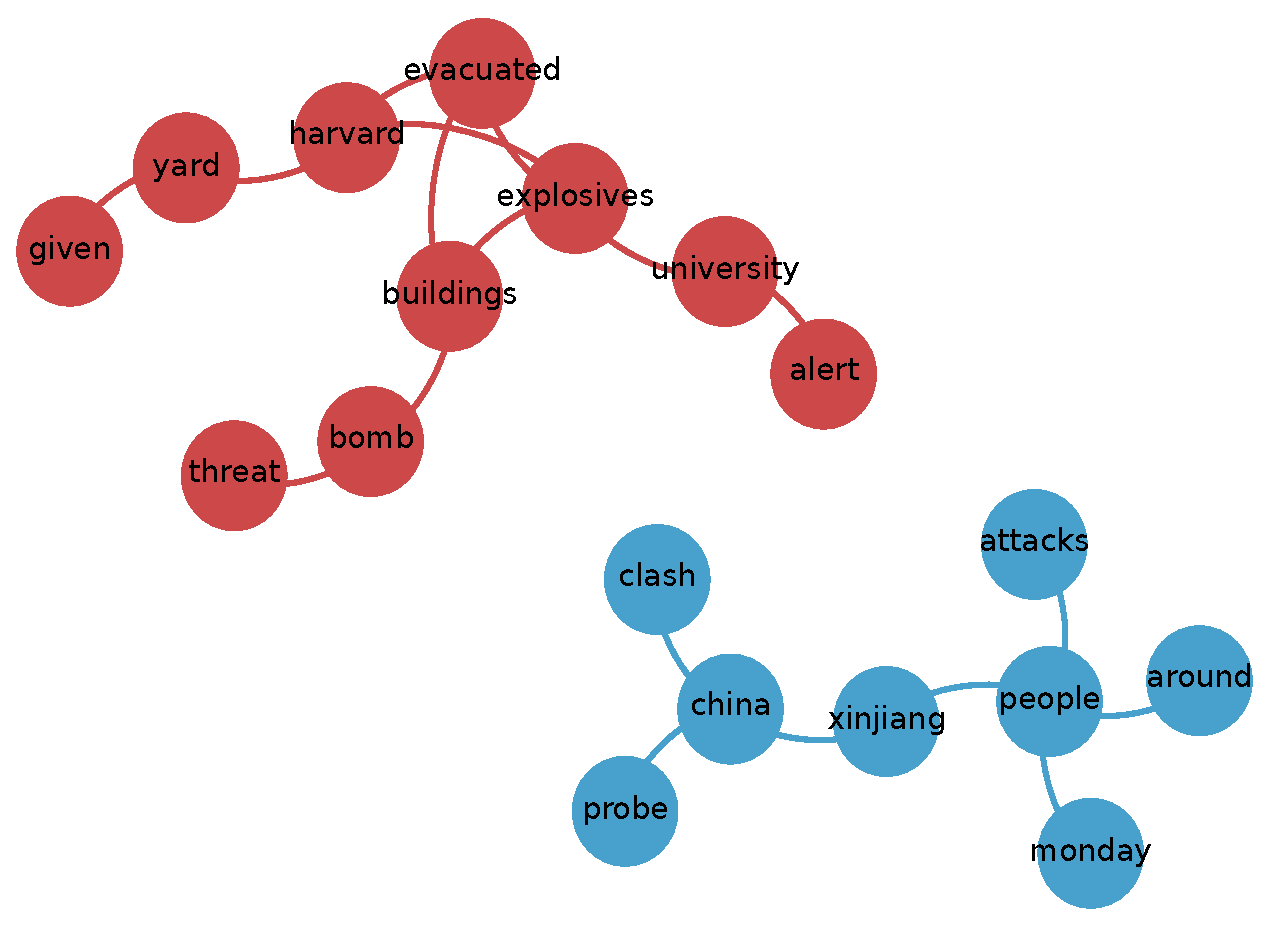
\includegraphics[width=.6\textwidth]{figures/data/connected_components.eps}
    \caption[Example of connected components]
    {Example of connected components. Two keyword sets are joined if they share
    at least one keyword in common.}\label{fig:connected-component}
\end{figure}



\section{Data Cleaning and Validation}\label{sec:cleaning}

There are two issues in our methodology: domain-specific stopwords and very old
tweets.

First, the event identification methodology does not take into account the use
of common words in the headlines. 
%
After removing the typical stopwords (words like ``the'', ``is'', ``do'', etc.),
some other common words appear in the headlines. 
%
Those words can be selected as the keywords for some news events, and by being
common, can join unrelated events together.
%
For example, words like ``update'' or ``breaking'' are commonly used by
different news sources. 
%
We validated our methodology by comparing the resulting events with random
events, those resulting from joining random keyword sets.

Second, due to the REST API behavior, some tweets are very old with respect to
the corresponding event. 
%
Sometimes the tweets are months or even years old. 
%
For that reason, we remove all tweets that were more than ten days old from the
date of the event. 

The event durations are then analyzed in order to verify if including the first
portion of the data, for each news event, makes sense in terms of their
duration. 
%
For instance, the time span in the first 5\% of the total amount of tweets
should be as half as the time of the first 10\%, one quarter of the 20\%, and so
on. 
%
For example, for some event a tweet from two years ago is retrieved, and the
remaining tweets are retrieved from a period of only two hours. 
%
Then the first 5\% of the tweets would be significantly larger than the rest
95\% in terms of time duration of the event. 



\subsection{Detecting Articulation Words}

A problem due to the methodology of identifying events is that some events can
join two unrelated news events together. 
%
This happens when two or more headlines from different events share a common
keyword. 
%
We performed a simple approach to identify such words and remove them from the
process.

Typical stopwords were removed when detecting groups of keywords to perform
searches, but some other words were common among the news accounts queried. 
%
For example, words like ``watch'', ``live'', or ``update'' are common to express
things like ``watch this video'', ``we are live on TV'', or to update a previous
headline with more info about it. 
%
By being common to different events (for example: ``Watch Jim Harbaugh's press
conference
live''\footnote{\url{https://twitter.com/49ers/status/519202023628374016}}  and
``WATCH LIVE: Of the 48 people being monitored for contact with Dallas patient,
no one is showing any
symptoms''\footnote{\url{https://twitter.com/PzFeed/status/519203692898435072}}),
they can end up in unrelated events by joining the keywords by those stopwords.


One approach to dealing with this problem is to have a pre-defined list of
stopwords to remove from the stream of headlines. 
%
Although we do not know beforehand which words those are. 
%
We call such words \emph{articulation words} in the sense that if they appear as
keywords after processing a group of headlines, then when joining the searches
together, those words would join unrelated events. 
%
To identify a group of those keywords, we used a modified
\emph{tf-idf}~\cite{sparck1972statistical} to detect them from the headlines.

The modified version of \emph{tf-idf}, what we refer as \emph{maxtf-idf}, is
meant to assign more weight to the terms that are frequent in any document. 
%
For instance, \emph{tf-idf} of a term in a document tries to assign a weight
related to how ``rare'' is that term in the whole collection, and how frequent
is in that document, by indicating how representative the term is with respect
to the document. 
%
On the other hand, what we want to achieve is to weigh a term more if the term
is more frequent in any document, relative to the frequency in the current
document. 
%
With that in mind, we want to identify terms that might be ``adding noise'' to
the corpus, and hence, to join unrelated events together.

The definition of \emph{maxtf} is as follows:

\begin{equation}
\text{maxtf}(t,\mathit{d},D) = 0.5 + \frac{0.5 + max\{f(t,\mathit{d}') : \mathit{d}' \in D\}}{max\{f(w,\mathit{d}) : w \in \mathit{d}\}}
\end{equation}

and for \emph{idf}, the usual formula:

\begin{equation}
\text{idf}(t,D) = \log\frac{N}{|\{\mathit{d} \in D : t \in \mathit{d}\}|}
\end{equation}

\noindent where $t$ is a term, $\mathit{d}$ is a document, and $D$ is the corpus
of documents. 
%
In this case, we set $t$ as a keyword, $\mathit{d}$ as the set of keywords of
one hour, and $D$ the set of documents of that day.

\begin{figure}
\begin{center}
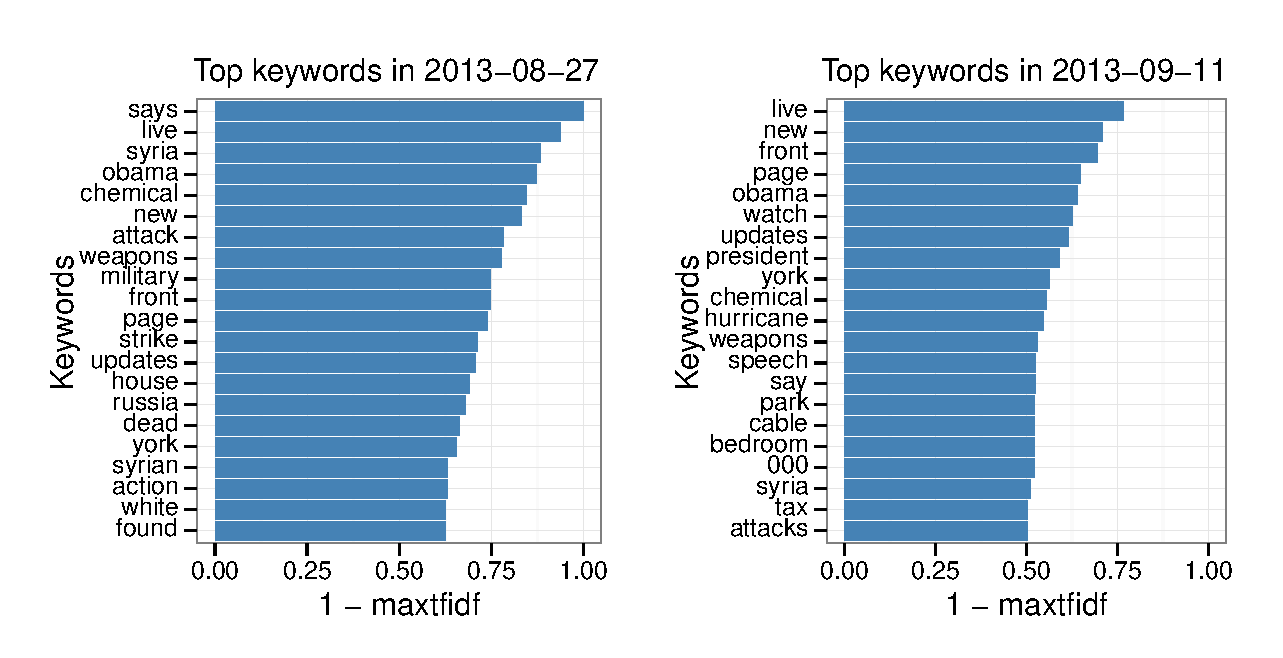
\includegraphics[width=\textwidth]{figures/data/stopwords}
\caption[Stopwords detection.]{Stopwords detection. Normalized
  $1-\text{maxtf-idf}$ score for data from August 27th (left) and August 28th
  (right) of 2013. The top score words for both plots are ``says'' and ``live''.
  We used the top score words to disconnect connected components of events. The
  title indicates the date when those keywords were identified, while the number
  beside corresponds to the total number of keywords.}
\label{fig:stopwords}
\end{center}
\end{figure}


After identifying such words, the idea was to disconnect the components
connected by those words. 
%
The process was to disconnect each component by the word with top normalized
$1-\text{maxtf-idf}$ score each time until the component could not be
disconnected further. 
%
We ended by adding the top score words to a list of banned words which were
ignored from subsequent runs of the data collection methodology. 
%
In Figure~\ref{fig:stopwords} there are two examples of this process to identify
the words.


\subsection{Validation of Event Modeling}\label{sub:valcoll}

In order to validate the results of the events identification process, we
compared our results with a baseline consisting on randomly generated events.

We generated artificially connected components taking randomly searches from the
first stage, and then merging their tweets to generate a ``random'' connected
component. 
%
The assumption here is that the tweets of a search are closely related to its
pair of keywords. 
%
From that, we wanted to ensure that the identified events make sense by
comparing them with random components. 
%
The idea is that using the connected components approach would join related
events together, so it would suffice to compare to a random baseline.

\begin{figure}
\begin{center}
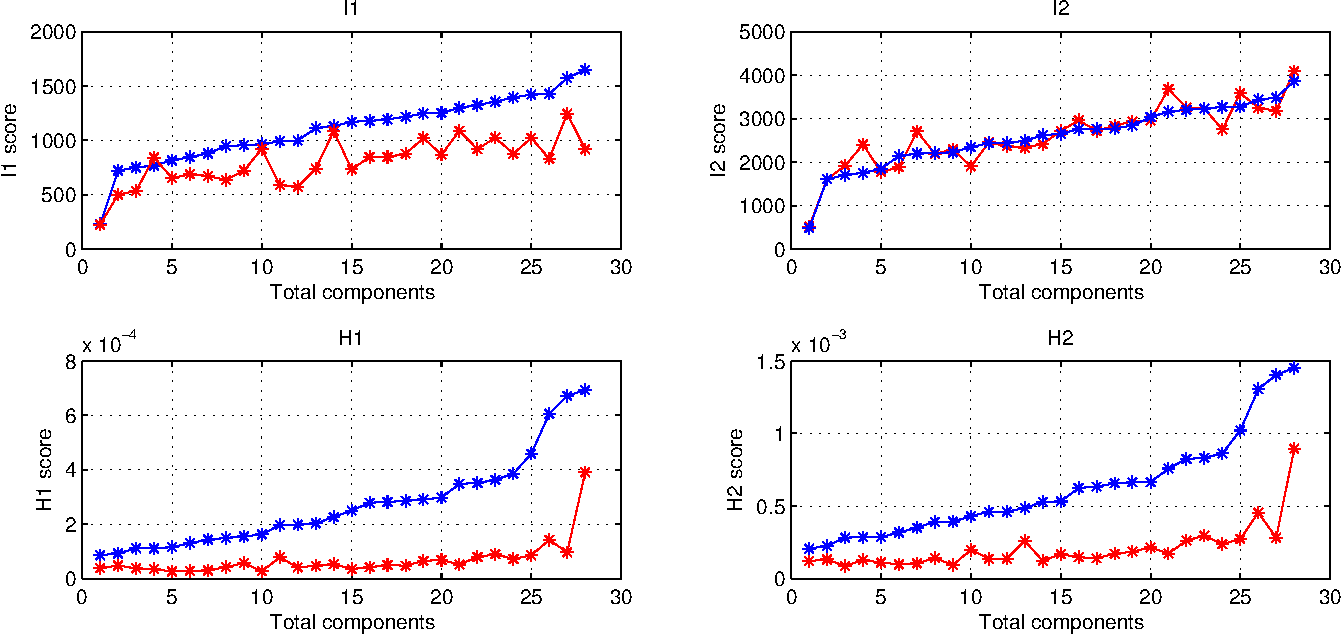
\includegraphics[width=.8\textwidth]{figures/data/connected_components_validation2.pdf}
\caption[Validation of connected components] {Validation of connected
  components. Each plot in this figure compares the quality of the cluster of
  tweets obtained from connected components and random components. The blue line
  corresponds to our approach, while the red line corresponds to the random
  components baseline. For visual clarity, the values obtained from connected
  components were sorted in ascending order, hence the blue line is
  monotonically increasing. The values obtained were rearranged in the same
  order as well.}\label{fig:connected_components_validation} 
\end{center}
\end{figure}

\begin{table}
\centering
\begin{tabular}{| c | c | c |}
\hline
Name & Metric & Meaning \\
\hline
\hline
$I_1$ & $\sum_{i=1}^k \frac{1}{n_i} \sum_{(u,v) \in S_i} \text{sim}(u,v)$ & Higher value is better\\
\hline
$I_2$ & $\sum_{i=1}^k \sqrt{ \sum_{(u,v) \in S_i} \text{sim}(u,v)}$ & Higher value is better \\
\hline
$E_1$ & $\sum_{i=1}^{k} n_i \frac{\sum_{v \in S_i, u \in S} \text{sim}(u,v)}{\sqrt{\sum_{(u,v) \in S_i} \text{sim}(u,v)}}$ & Lower value is better \\
\hline
$G_1$ & $\sum_{i=1}^k \frac{\sum_{v \in S_i, u \in S}\text{sim}(u,v)}{\sum_{(v,u) \in S}\text{sim}(v,u)}$ & Lower value is better \\
\hline
$G_1^{'}$ & $\sum_{i=1}^k n_i^2 \frac{\sum_{v \in S_i, u \in S}\text{sim}(v,u)}{\sum_{(u,v) \in S_i}\text{sim}(u,v)}$ & Lower value is better \\
\hline
$H_1$ & $\frac{I_1}{E_1}$ & Higher value is better \\
\hline
$H_2$ & $\frac{I_2}{E_1}$ & Higher value is better \\
\hline
\end{tabular}
\caption[Clustering metrics used for validation]{Clustering metrics used for
  validation. This table lists the clustering metrics used in Figure
  \ref{fig:connected_components_validation}. Those formulas correspond to usual
  clustering evaluation metrics, like inter-cluster similarity ($I_1, I_2$),
  intra-cluster similarity ($E_1, G_1, G_1'$) and similarity radio ($H_1, H_2$).
  In $I_1, I_2, H_1, H_2$ a higher value is better.  In $G_1, G_1^{'}$, lower
  value is better. }
\label{table:clustering_metrics}
\end{table}

We calculate standard internal clustering metrics (listed in
Table~\ref{table:clustering_metrics}) over the found components and on the
random components and then compare their results. 
%
The comparisons were made by taking components of the same size (in terms of
keywords and tweets, taking samples of tweets). 
%
Essentially, considering a component as a cluster, the metrics evaluate the
similarity intra- and inter-clusters. 
%
We compare the metrics against random clusters to see if our approach tends to
join related events together, compared to a baseline.
%
Equal results means that our approach is no better than joining searches
randomly. 
%
The results by metric are shown in
Figure~\ref{fig:connected_components_validation}. For almost every metric, our
approach is better than random.


\subsection{Events duration}\label{sub:dur}

Due to the capabilities of the REST API, the tweets collected can be older than
the actual date of the event detected. 
%
For that reason, some tweets can be very old and not relevant to the event
itself. 
%
Furthermore, when a retweet is collected by the process, also the original tweet
is stored\footnote{The data of the original tweet is included in the data of the
retweet}. 
%
This could be a problem especially when we want to perform predictions using the
first part of the data. 

\begin{figure}
\centering
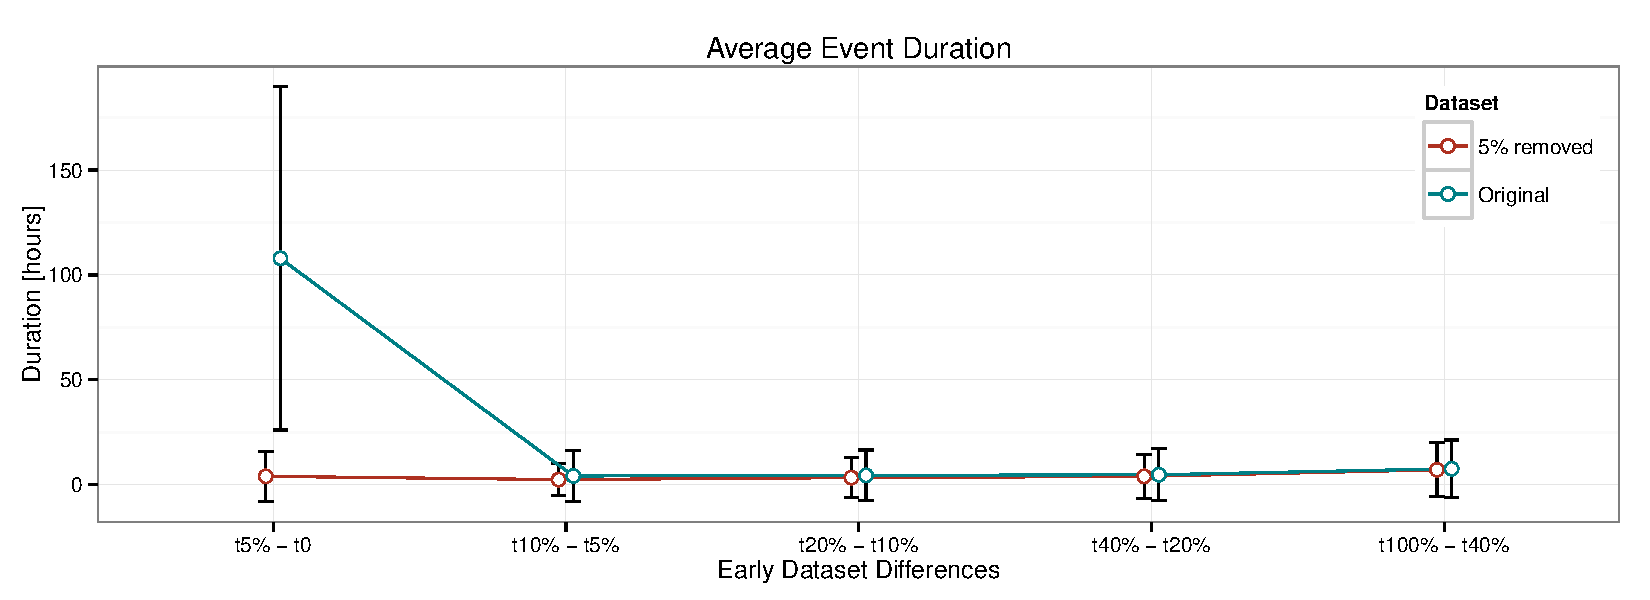
\includegraphics[width=\textwidth]{figures/data/duration-differences.pdf}
\caption[Duration differences of events.]{Duration differences of events. The
  $x$-axis represents the categories of datasets: the first one (t5\%-t0)
  represents the difference of time between the timestamp of the oldest tweet
  and the newest tweet on the first 5\% of the tweets. The next one (t10\%-t5\%)
  corresponds to the difference between the newest tweet in the first 10\% and
  the newest tweet on the first 5\% of data, etc. After removing the first 5\%
  of data, the time differences are roughly the same across all
  datasets.}\label{fig:duration-differences}

\end{figure}

After collecting tweets for an event, we remove the first 5\% of tweets of each
event, in addition to restrict tweets of an event up to ten days before the day
of its publication. 
%
We saw that the first 5\% of the tweets cover the largest amount of time on all
events, due to the problems exposed above. 
%
After removing the first 5\%, the events duration were more consistent (the
first 10\% covers twice the amount of time that the first 5\% covers, and so
on). 
%
Figure~\ref{fig:duration-differences} shows the effect of removing the first 5\%
of data by calculating the time differences between the timestamps of the tweets
at the ends of each dataset.


\begin{figure}
  \centering
  \begin{subfigure}{\textwidth}
    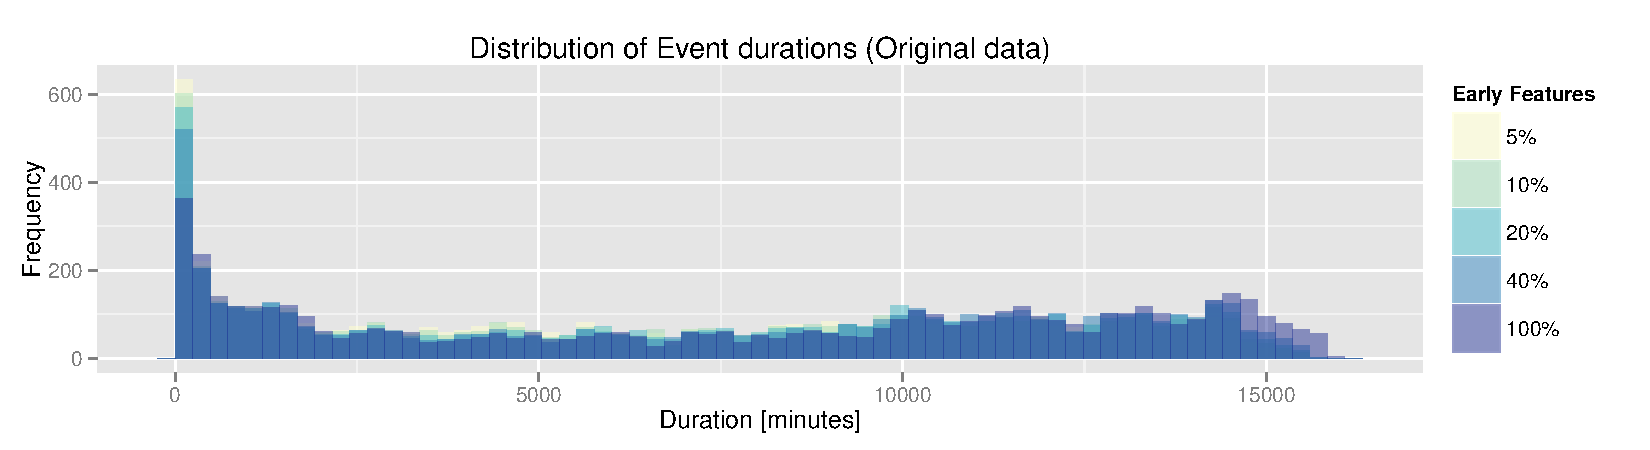
\includegraphics[width=\textwidth]{figures/data/dist-events-durations-o.pdf}
    \caption[Distribution of events duration on the original
      dataset.]{Distribution of events duration on the original dataset.} 
    \label{sfig:dist-events-durations-o}
  \end{subfigure}

  \begin{subfigure}{\textwidth}
    \centering
    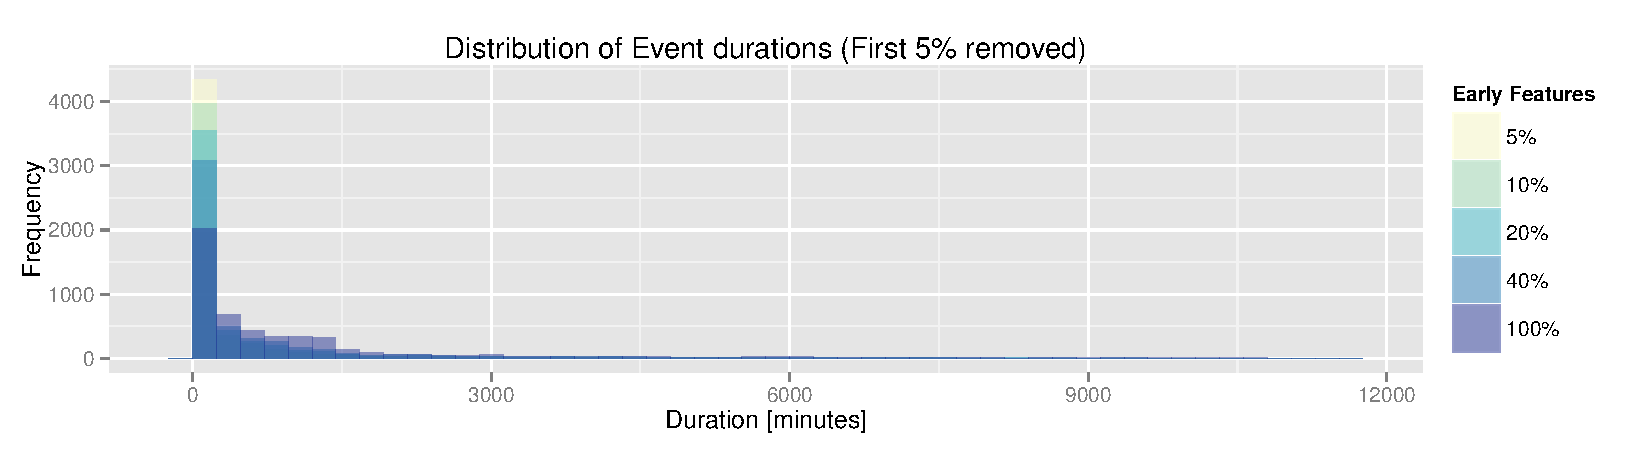
\includegraphics[width=\textwidth]{figures/data/dist-events-durations-5.pdf}
    \caption[Distribution of events duration on the 5\%-trimmed
      dataset.]{Distribution of events duration on the 5\%-trimmed dataset.} 
    \label{sfig:dist-events-durations-5}
  \end{subfigure}

  \caption[Distribution of events duration]{Distribution of events duration. In
    (a) it can be seen that there are a non negligible amount of events with a
    high duration (between 7 and 10 days). In (b), we see a clearer power law on
    the distribution of events after removing the first 5\% of tweets.}
  \label{fig:dist-events-durations}
\end{figure}

Events duration distributions are shown in
Figure~\ref{fig:dist-events-durations}. 
%
It can be seen in Figure~\ref{sfig:dist-events-durations-o} that there is a non
negligible amount of events with a duration between 7 and 10 days. 
%
By considering the first 5\% of tweets from those events, the oldest tweets will
correspond to situations when the event has not already happened yet, and it
will lead to errors or incorrect results. 
%
Removing the first 5\% produces a cleaner dataset, as shown in
Figure~\ref{sfig:dist-events-durations-5}.


%%%
\paragraph{Summary.}
%
Our data collection methodology consists of a pipeline starting at headline
retrieval from manually selected news sources, ending with event identification.

An event is a set of keywords with a set of tweets that talk about these
keywords.
%
The keywords can be seen as the event representatives. 
%
For example, the event \{chile, northern, iquique, tsunami, struck, warning,
earthquake, magnitude\} describes an earthquake that occurred in Chile on April
2th. 
%
However, a few challenges had to be addressed from this methodology.

Some keywords are common across several distinct events. 
%
For that reason, it was necessary to identify such words and remove them from
the keywords detection phase, for example, words like ``update'', ``watch'', or
``live'', which do not add any value to the meaning of any event. 

Finally, due to the nature of the methodology proposed, the tweet sets had to be
trimmed because of their long duration. 
%
Because of the Twitter REST API, sometimes tweets from long ago were retrieved,
but since they add only noise to our dataset, they were removed.


\chapter{User Reaction: Predicting and Characterizing High-Activity News Events} 
\label{chapter:high-activity}

\section{Introduction}

Users publish a high volume of information about real-world events on social
media almost instantly.
%
This makes social media a primary source for breaking news.
%
Some of these real-world events can end up having a very strong impact on the
network.  
%
The effect of such events can be analyzed from several perspectives, one of them
being the intensity and characteristics of the collective activity that it
produces in the social platform. 
%
We research 5,234 real-world news events encompassing 43 million messages
discussed on the Twitter microblogging service for approximately 1 year, using a
portion of the dataset collected via the methodology described in
Chapter~\ref{chapter:data}.
%
We show empirically that exogenous news events naturally create collective
patterns of bursty behavior in combination with long periods of inactivity in
the network. 
%
This type of behavior agrees with other patterns previously observed in other
types of natural collective phenomena, as well as in individual human
communications. 
%
In addition, we propose a methodology to classify news events according to the
different levels of intensity in activity that they produce. 
%
In particular, we analyze the most highly active events and observe a consistent
and strikingly different collective reaction from users when they are exposed to
such events. 
%
This reaction is independent of an event's reach and scope.  
%
We further observe that extremely high-activity events have characteristics that
are quite distinguishable at the beginning stages of their outbreak.  
%
This allows us to predict with high precision, the top 8\% of events that will
have the most impact in the social network by just using the first 5\% of the
information of an event's lifetime evolution. 
%
This strongly implies that high-activity events are naturally prioritized
collectively by the social network, engaging users early on, way before they are
brought to the mainstream audience.


% Motivation

Social media is now a primary source of breaking news information for millions
of users all over the
world~\cite{Kwak:2010,petrovic2013can,broersma2013twitter,tandoc2016most,Rogers:2013:DTT:2464464.2464511}.
%
Social media along with mobile internet devices have crowd-sourced the
task of disseminating real-time information. 
%
As a result, both news media and news consumers have become inundated with much
more information than they can process. 
%
One possible way of handling this data overload is to find ways to filter and
prioritize information that has the potential of creating a strong collective
impact. 
%
Understanding and quickly identifying the type of reaction that certain
exogenous events will produce in social media, at both global and
local scales, can help in the understanding of collective human behavior.
%
This may improve information delivery, journalistic coverage and
crisis management, among other things. 
%
We address this challenge by analyzing the properties of real-world news events
in social media, showing that they corroborate patterns previously identified in
other case studies of human communications. 
%
In addition, we present our main findings of how news events that produce
extremely high-activity can be clearly identified in the early stages of their
outbreak.

% when
% consulting journalists on how news media sources measure the impact of
% news, we learn that they too face the issue of not having a clear way
% to approach this problem.

% Our contributions

%\newtext{

\paragraph{Contributions.} Our work focuses on high-activity events in social
media produced by real-world news, with the following contributions:
\begin{enumerate}

\item We introduce a methodology for modeling and classifying events in social
media, based on the intensity of the activity that they produce. 
%
This methodology is independent of the size and scope of the event, and is an
indicator of the impact that the event information had on the social network.

\item We show empirically that real-world news events produce collective
patterns of bursty behavior in the social network, in combination with long periods of
inactivity. 
%
Furthermore, we identify events for which most of their activity is concentrated
into very high-activity periods; we call these events {\em high-activity
events}.

\item We determine the existence of unique characteristics that differentiate
how high-activity events propagate in the social network.

\item We show that an important portion of high-activity events can be predicted
very early in their life-cycle, indicating that this type of information is
spontaneously identified and filtered collectively, early on, by social network
users.

\end{enumerate}
%}

%We focus on high-impact news events in social media, contributing by (i)
%\textcolor{blue}{defining a new concise way for measuring information impact that
%is independent of the size (whether large or small) and scope (whether
%local or global) of the event, but is representative of the urgency
%and immediacy of the reaction of users on the social media} (ii)
%determining the existence of unique characteristics that differentiate
%how high-impact exogenous events are propagated in the network, and
%(iii) show, through the creation of an early prediction model for
%high-impact events, that these types of news events are naturally
%identified and filtered by the network at very early stages of their
%outbreak.
\section{The VQ-Event Model}
 
As stated in the Introduction of this dissertation, we define an {\bf event} as
a conglomerate of information that encompasses all of the social media content
related to a real-world news occurrence. 
%
Using this specification, which considers an event as a complex unit of
information, we study the type of collective reaction produced by the event on
the social network. 
%
In particular, we analyze the intensity or immediacy of the
social network's response. 
%
By analyzing the levels of intensity in activity induced by different exogenous
events to the network, we are implicitly studying the priority that has been
collectively assigned to the event by groups of independent individuals
\cite{barabasi2005origin, karsai2012universal}. 

We characterize an event's discrete activity dynamics by using
\emph{inter-arrival times} between consecutive social media messages within an
event (e.g., $d_i = t_{i+1}-t_i$, where $d_i$ denotes the inter-arrival time
between two consecutive social media messages $i$ and $i+1$ that arrived in
moments $t_i$ and $t_{i+1}$, respectively).


% We introduce a novel vectorial representation based on a {\em vector
% quantization of the interarrival time distribution}, which we call {\em
% ``VQ-event model''}. 
% %
We introduce a novel vectorial representation based on a vector quantization of
the inter-arrival time distribution, which we call ``VQ-event model". 
%
This model is designed to filter events based on the distribution of the
inter-arrival times between consecutive messages.  
%
The most representative inter-arrival times are learned from a large training
corpus. 
%
This approach is inspired by the {\em code-book-based representation} from the
field of multimedia content analysis, which has been used in audio processing
and computer vision~\cite{ff,Vaizman}.
%
In our proposed approach, our method learns a set of the most representative
inter-arrival times from a large training corpus of events; 
%
each one of the representative inter-arrival times is known as a {\em codeword}
and the complete learned set is known as the {\em code-book}~\cite{Vaizman}. 
%
Each event is then modeled using a vector quantization (VQ) that converts the
inter-arrival times of an event into a discrete set of values, each value
corresponding to the closest codeword in the code-book. 
%
The resulting VQ-event model is then a vector in which each dimension contains
the percentage of inter-arrival times of the event that were assigned a
particular codeword in the code-book.

%%

The VQ-event representation is relative to an event's overall size since the
model is normalized with respect to the number of messages in the event.
%
Therefore the only criteria that are considered in the model are the
inter-arrival times of each particular event. 
%
This model allows us to group events based on the {\em similarity of the
distribution} of their inter-arrival times. 
%
In those terms, we consider as high-activity events those events for which the
distribution of inter-arrival times is most heavily skewed towards the smallest
possible interval, zero. 
%
In other words, events for which the overall activity is extremely intense in
comparison with other events.

%%

We represent an event $\mathit{e}$, belonging to a collection of events
$\mathcal{E}$, as a tuple $(\mathcal{K}_\mathit{e}, \mathcal{M}_\mathit{e})$,
where $\mathcal{K}_\mathit{e}$ is a set of \emph{keywords} and
$\mathcal{M}_\mathit{e}$ is a set of \emph{social media messages}.
%
Both the keywords and the messages are related to a real-world occurrence. 
%
The keywords are extracted in order to succinctly describe the occurrence, and
the messages are posts from users about the event.

%%\mathit{i}

To learn the most representative inter-arrival times we perform the following:
%
for each $\mathit{e} \in \mathcal{E}$ with messages $\mathcal{M}_\mathit{e} =
\lbrack m_{1}^\mathit{e}, m_{2}^\mathit{e}, \ldots m_{n}^\mathit{e} \rbrack$ and
their corresponding time-stamps $\lbrack t_{1}^\mathit{e}, t_{2}^\mathit{e},
\ldots t_{n}^\mathit{e} \rbrack$ where $t_{\mathit{i}} \leq t_{\mathit{i}+1}
\forall \mathit{i} \in [1,n]$, we compute all the inter-arrival times
$d_{\mathit{i}}^\mathit{e} =
t_{\mathit{i}}^\mathit{e}-t_{\mathit{i}-1}^\mathit{e}$ (the value of $t_{0}$ is
considered equal to $t_{1}$ for initialization purposes). 
%
Then, the values of $d_{\mathit{i}}^\mathit{e}$ for all events in $\mathcal{E}$
are clustered to identify the {\em most representative} inter-arrival times.

%%

Once the most representative inter-arrival times have been learned, the vector
quantization for each event is produced as follows: 
%
for each event, obtain all the inter-arrival times, and quantize each of the
inter-arrival times to the closest codeword in the code-book.  
%
This process is summarized in Algorithm~\ref{alg:learn_representation}.
%
Line~\ref{alg:line:all_time_diff} collects all of the inter-arrival times for all
the events in $\mathcal{E}$ in \textbf{f}. 
%
Line~\ref{alg:line:cluster} is a clustering algorithm which takes \textbf{f} and
the number of clusters $k$ as inputs and returns the centroids of the clusters
as the output in \textbf{c}. 
%
The centroids can be thought of as the most representative inter-arrival times
for the event set $\mathcal{E}$. 
%
After that, the inter-arrival times of each event $e$ is vector quantized in
terms of the centroids to obtain a $k$-dimensional real valued representation of
the event (Line~\ref{alg:line:vq}). 
%
In this representation, each entry is the percentage of messages with that
particular codeword as the inter-arrival time.

\begin{algorithm}
  \caption{{\scshape Learn-VQ-Representation}$(\mathcal{E}, k)$}
  \label{alg:learn_representation}
  \begin{algorithmic}[1]
    \STATE $\textbf{f} \gets \{d_{i}^\mathit{e}\text{ } | \text{ } m_{\mathit{i}}^\mathit{e} \in
    \mathcal{M}_\mathit{e}, \mathit{e} \in \mathcal{E} \}$ \label{alg:line:all_time_diff}
    \STATE \textbf{c} $\gets$ {\tt cluster(}$\textbf{f}, k${\tt)} \label{alg:line:cluster}
    \FOR{$\mathit{e} \in \mathcal{E}$} 
      \STATE \textbf{\textit{e}} $\gets$ {\tt vq(}$d_{i}^\mathit{e}, \textbf{c}${\tt)}\\ \label{alg:line:vq}
    \ENDFOR
    \RETURN A representation in $\mathbb{R}^{k}$ of each event $\mathit{e} = (\mathcal{K}_\mathit{e}, \mathcal{M}_e) \in \mathcal{E}$.
  \end{algorithmic}
\end{algorithm}

%\mathit{e}
% \todo[inline]{uniforme con algoritmo en Background}
% \begin{algorithm}
%   \caption{{\tt learn\_representation()}}
%   \label{alg:learn_representation}
%   \begin{algorithmic}[1]
%     \REQUIRE Event set $\mathcal{E}$, and number of codewords $k$ in the codebook.\\
%     \ENSURE A representation in $\mathbb{R}^{k}$ of each event $\mathit{e} = (\mathcal{K}_\mathit{e}, \mathcal{M}_e) \in \mathcal{E}$.\\
%     \STATE $\textbf{f} \leftarrow \{d_{i}^\mathit{e}| m_{\mathit{i}}^\mathit{e} \in
%     \mathcal{M}_\mathit{e}, \mathit{e} \in \mathcal{E} \}$
%     \\ \label{alg:line:all_time_diff} \STATE \textbf{c} $\leftarrow$
%     {\tt cluster(}$\textbf{f}, k${\tt)} \label{alg:line:cluster}
%     \FOR{$\mathit{e} \in \mathcal{E}$} \STATE \textbf{\textit{e}} $\leftarrow$ {\tt
%       vq(}$d_{i}^\mathit{e}, \textbf{c}${\tt)}\\ \label{alg:line:vq}
%     \ENDFOR
%   \end{algorithmic}
% \end{algorithm}

%%

To illustrate events with different levels of intensity in activity we present
two examples taken from our analysis of Twitter data. 
%
These examples show the inter-arrival time histograms for the entire life-cycle of
the two events. 
%
In the first example, the majority of the messages about the death of political
leader Nelson Mandela (Figure~\ref{fig:hi:example-mandela}) arrive within almost
zero seconds of each other. 
%
On the contrary, the messages about The Oscars
(Figure~\ref{fig:hi:example-oscars}) are much more spread out in time.

%%

We note that, by using inter-arrival times to describe the intensity of the
activity of an event, we make our analysis independent of the particular
evolution of each event. 
%
By doing this, we put no restrictions on how high-activity events unfold in
time, for example, they could be: 
%
(a) events that start out slowly and suddenly gain momentum, 
%
(b) events that go viral soon after they appear on social media and then decay
in intensity over a long (or short) period of time, 
%
(c) events that from the beginning produce large amounts of interest and sustain
that interest throughout their long (or short) lifespan, or 
%
(d) events that are a concatenation of any of the above, etc.


\section{Experimental Analysis}

We study a dataset of news events gathered from news headlines from a
\emph{manually curated} list of well-known news media accounts (e.g., @CNN,
@BreakingNews, @BBCNews, etc.) in the microblogging platform
Twitter~\cite{twitter}.
%
Headlines were collected periodically every hour, over the course of
approximately one year. 
%
In parallel, all the Twitter messages were extracted for each news event using
the public API \cite{twitterapi}.
%
This process was performed by automatically extracting descriptive sets of
keywords for each event using a variation of frequent itemset
extraction~\cite{Tan_Steinbach_Kumar} over the event's headlines. 
%
These sets of keywords were then used to retrieve corresponding user tweets for
each event. 
%
We validate the events gathered in our data collection process to ensure that
each group of social media posts corresponds to a meaningful and cohesive news
event. 
%
We provide a detailed description of the collection methodology and of
the validation of event cohesiveness in Chapter~\ref{chapter:data}.
%
Overall, the resulting dataset contains $43,256,261$ tweets that account for
$5,234$ events (Table~\ref{table:hi:dataset-stats}).


\begin{table}
  \centering
  \begin{tabularx}{\textwidth}{@{}p{6cm}llll@{}}
    \toprule
    \textbf{News events' property} & \textbf{Minimum} & \textbf{Mean} & \textbf{Median} & \textbf{Maximum} \\ \midrule
    \# of posts & 1,000 & 8,254 & 2,474 & 510,920 \\
    \# of keywords & 2 & 3.77 & 3 & 39 \\
    Event duration (hours) & 0.12 & 20.93 & 7.46 & 190.43 \\ \bottomrule
  \end{tabularx}
  \caption{High-level description of the dataset of news events.} 
  \label{table:hi:dataset-stats}
\end{table}



In Figure~\ref{fig:hi:components} we characterize an example event from our
dataset, by showing the set of keywords and a sample of tweets associated to the
event. 
%
These keywords form a semantically meaningful event; they refer to the incident
where soccer player Luis Suarez was charged for biting another player during the
FIFA World Cup in 2014. 
%
This general collection process results in a set of social media posts
associated to an event which can encompass several memes, viral tweets and
pieces of information. 
%
Therefore, an event is composed of diverse information, addressing more
heterogeneous content than prior
work~\cite{Castillo:2014,Szabo:2010,Lerman:2010,Tatar:2011,Pinto:2013,Ahmed:2013,suh2010want}
which focus on single pieces of information (e.g., a particular meme, a viral
tweet etc.).


\begin{figure}
  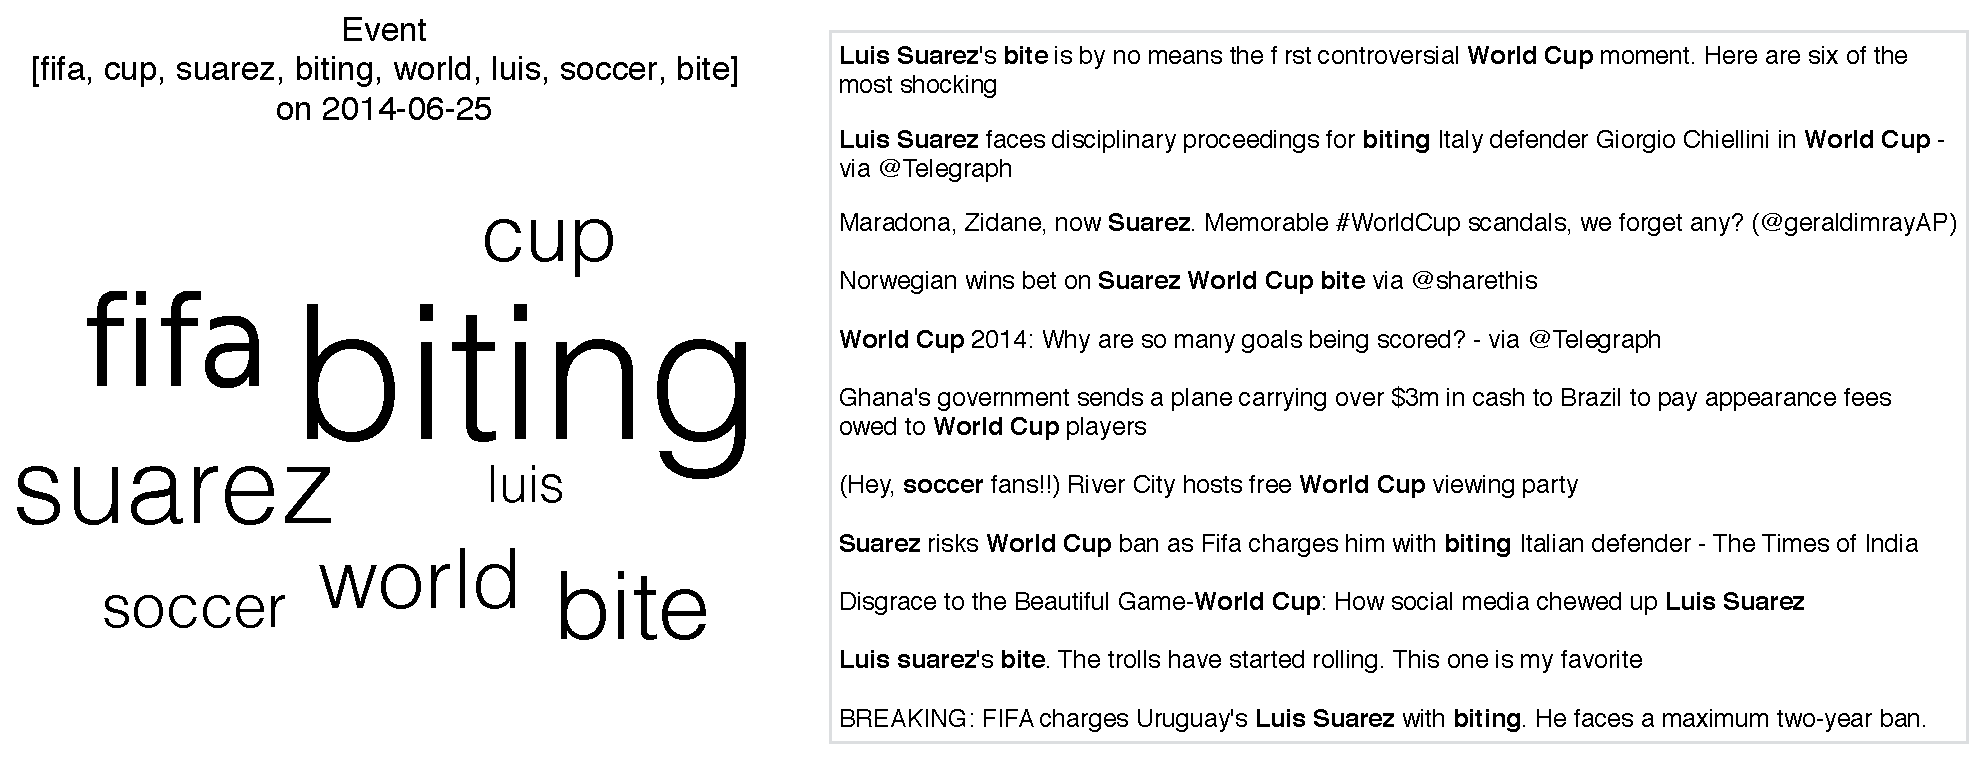
\includegraphics[width=\textwidth]{figures/high-activity/fig2}
  \caption[Example event]{A representative event, collected on 2014-06-25 with
      keywords (left) and sample user posts (right) collected from the Twitter
      Search API. Collected user posts contain at least one pair of keywords. }
  \label{fig:hi:components}
\end{figure}


The collection of events is converted into their VQ-event model representation. 
%
Using this model, we can identify events that have produced similar levels of
activity in the social network. 
%
In other words, events are considered to have similar activity if the
inter-arrival times between their social media posts are similarly distributed,
implying a very much alike collective reaction from users to the events within a
group. 
%
In order to identify groups of similar events, we cluster the event models. 
%
We sort the resulting groups of events from highest to lowest activity,
according to the concentration of social media posts in the bins that correspond
to short inter-arrival times. 
%
We consider the events that fall in the top cluster to be high-activity events
as most of their inter-arrival times are concentrated in the smallest interval of
the VQ-event model.
%
In our dataset, these correspond to roughly 8\% of the events. 
%
We consider the next clusters in the sorted ranking to form medium-high activity
events, and so on. 
%
Thus we end with four groups of events: high, medium-high, medium-low and low.
Figure~\ref{fig:hi:heatmap} shows a heatmap of the inter-arrival relative
frequency for each cluster. 
%
This classification of events based on activity intensity is independent of
event size. 


\begin{figure}
  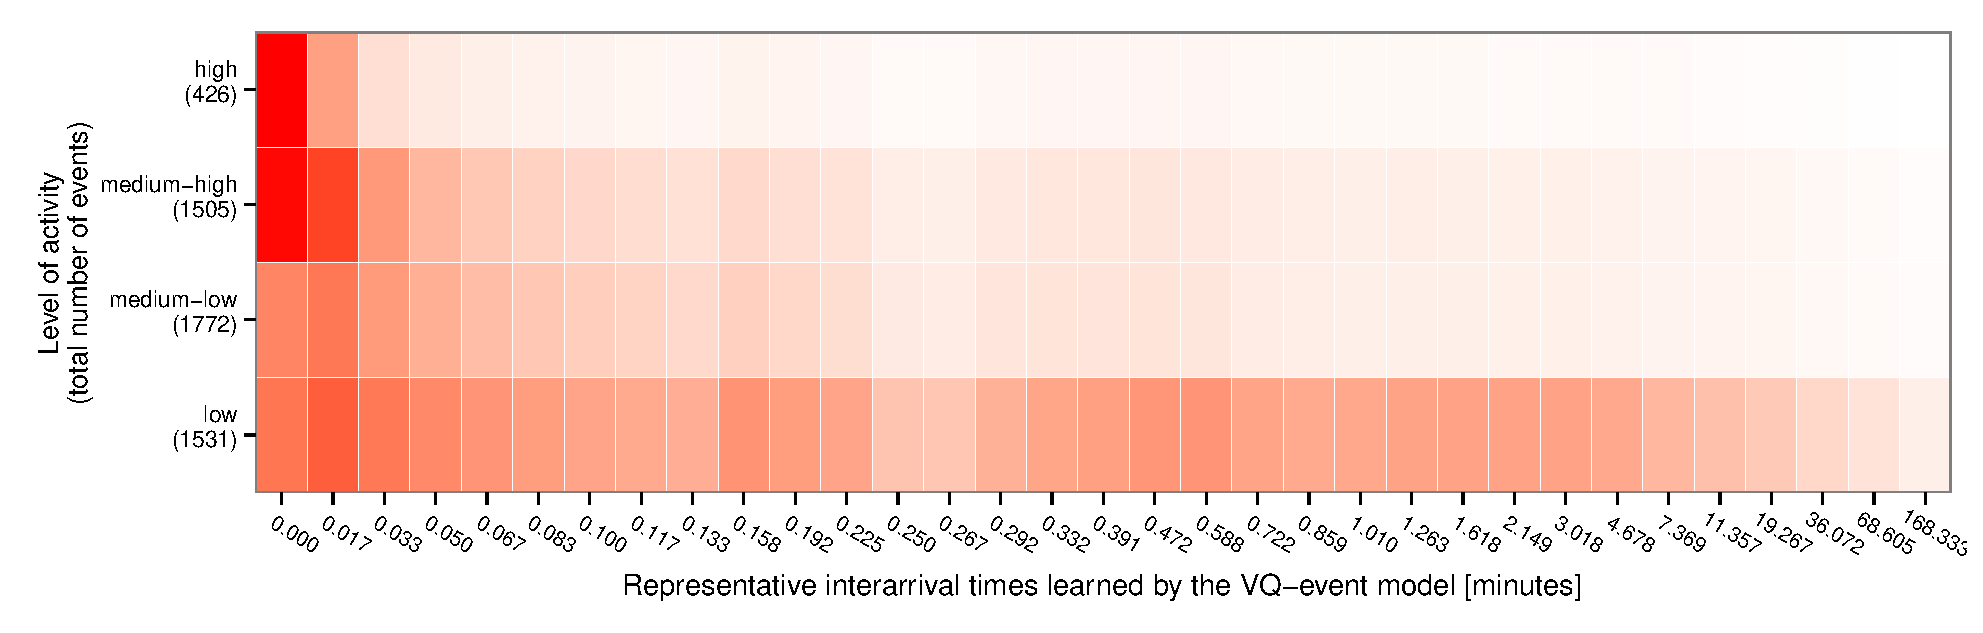
\includegraphics[width=\textwidth]{figures/high-activity/fig3}
  \caption[Heatmap of the categorization of events into clusters of
  activity.]{{Heatmap of the categorization of events into clusters of activity.
  Each row is the average representation of all the events in that clusters.  A
  darker cell represents a higher value. The y-axis specifies the number of
  events in that cluster. Clusters are (top to bottom): high-impact,
  medium-high, medium-low, and low.}}
  \label{fig:hi:heatmap}
\end{figure}
\section{Results and Discussion}

Our main objective in this work is to analyze the characteristics of
high-activity events which differentiate them from other types of events. 
%
In particular, we identify how early on in an event's life-cycle can we determine
if an event is going produce high activity in the online social network.


%\clearpage
\begin{table}
  \centering
  {\scriptsize
    \begin{tabular*}{1\linewidth}{p{5cm}p{5cm}}
      \toprule
      \textbf{Event} & \textbf{Sample Tweets} \\
      \midrule
      \pbox{20cm}{\textbf{Description:}\\ Death of South African\\ politician Nelson Mandela. \vspace{.1cm}\\
        \textbf{Keywords:}\\ {[}nelson, mandela{]}\vspace{.1cm}\\
        \textbf{Date:}\\ 2013-12-05 \vspace{.1cm}\\
        \textbf{Size:} \\ 134,637 tweets}
      & \pbox{20cm}{
        @DaniellePeazer: RIP Nelson Mandela..... what a truly phenomenal and\\ inspirational man xx\vspace{.1cm}\\
        @iansomerhalder: Im in tears.The world has lost one of its greatest shepherds \\of peace. Thank you Mr.Mandela for the love you radiated. http://t.co/u39MVVEKe8\vspace{.1cm}\\
        @FootballFunnys: This is so true. RIP Nelson Mandela. http://t.co/vF9xri8LdP\vspace{.1cm}\\
        @David\_Cameron: I've spoken to the Speaker and there will be statements \\and tributes to Nelson Mandela in the House on Monday.} \\
      \midrule
      \pbox{20cm}{\textbf{Description:}\\ 2013 Mumbai Gang Rape \vspace{.1cm}\\
        \textbf{Keywords:}\\ {[}rape, mumbai{]}\vspace{.1cm}\\
        \textbf{Date:}\\ 2013-08-24 \vspace{.1cm}\\
        \textbf{Size:} \\1,705 tweets}
      & \pbox{20cm}{
      % select user.screen_name, text from tweet join user on tweet.user_id_id = user.user_id where event_id_id = 272;
      @TheNewsRoundup: Mumbai gang-rape: Second accused confesses to crime: \\Mumbai Police - Daily News Analysis http://t.co/KnabwhqH66\vspace{.1cm}\\
      @vijayarumugam: An interesting take on the Mumbai rape: http://t.co/ylBmW4l8sA\vspace{.1cm}\\
      @LondonStephanie: Two arrested over gang rape of Mumbai photojournalist \\that sparked renewed protests in India http://t.co/McYfLNDvaE\vspace{.1cm}\\
      @GanapathyI: Most brutal rapist of Delhi gang-rape was 17. Most brutal rapist\\ of Mumbai gang-rape is 18. Worst Young generation I have seen in my life.}\\
%        @M\_arioBalotelli: CLEAR ANGLE of the Suarez bite!!  https://t.co/bI08YsZWSE\vspace{.1cm}\\
%        @fifamedia: Disciplinary proceedings opened against Uruguay's Luis Suarez\\ http://t.co/w6mRNuSGZt\vspace{.1cm}\\
%        @DeadlineDayLive: Luis Suarez will sign a 5-year contract at Barcelona and he'll wear \\the no. 9 shirt. (Source: http://t.co/6uRIUwjsGN) http://t.co/FxyOf9ERVr\vspace{.1cm}\\
%        @GeniusFootball: BREAKING: FIFA have caught Suarez leaving the stadium?\\ http://t.co/vsQQCVV1GQ} \\
      \bottomrule
    \end{tabular*}
  } \caption[Examples of high-activity events]{Examples of high-activity news
  events. The events shown were taken from the ``high'' category according to
  Figure~\ref{fig:hi:heatmap}.}
  \label{table:high-impact-sample}
\end{table}

\begin{table}
  \centering
  {\scriptsize
    \begin{tabular*}{1\linewidth}{p{5cm}p{5cm}}
      \toprule
      \textbf{Event} & \textbf{Sample Tweets} \\
      \midrule
      \pbox{20cm}{\textbf{Description:}\\Teen survives hiding \\in a plane wheel.\vspace{.1cm}\\
        \textbf{Keywords:}\\ {[}teen, survives, old, \\well, skydivers, plane, wheel, flight{]}\vspace{.1cm}\\
        \textbf{Date:}\\ 2014-04-21 \vspace{.1cm}\\
        \textbf{Size:}\\ 18,519}
      & \pbox{20cm}{
        %select user.screen_name, text from tweet join user on tweet.user_id_id = user.user_id where event_id_id in (22310,22274,22240);
        @ToniWoemmel: 16-year-old somehow survives flight from California to\\ Hawaii stowed away in planes wheel well: http://t.co/IGiJa60SiK\vspace{.1cm}\\
        @iOver\_think: 38,000 feet at -80F: Teen stowaway survives five-hour\\ California-to-Hawaii flight in wheel well http://t.co/ejXQH9VZyT\vspace{.1cm}\\
        @TruEntModels: GOD IS GOOD...runaway TEEN hid in plane's wheel for\\ 5 HOUR flight during FREEZING temps and survived http://t.co/6g6Cqhs9Ib\vspace{.1cm}\\
        @DvdVill: A 16-year-old kid, who was mad at his parents, hid inside a jet\\ wheel and survived flight to Hawaii. http://t.co/c82GbjrfUH\\
        %@guardiannews: Angela Merkel denied access to her NSA file http://t.co/FLQc0zSjYJ\vspace{.1cm}\\
        %@mog7546: \#GERMANY's \#Merkel says \#OBAMA's \#US assurances on \#NSA spying\\ "INSUFFICIENT" - Reuters India http://t.co/D2L52CP9YZ\vspace{.1cm}\\
        %@GermanyForum: Merkel denied access to own NSA file http://t.co/e6vKCOkbXA\vspace{.1cm}\\
        %@kgosztola: US ignores request from German Chancellor Angela \\Merkel to look at NSA file:\\ http://t.co/HFTMMZBu5W
      }
      \\
            \midrule
      \pbox{20cm}{\textbf{Description:}\\Surveying the damages of \\ recent tornado in Canada. \vspace{.1cm}\\
        \textbf{Keywords:}\\ {[}canada, tornado{]}\vspace{.1cm}\\
        \textbf{Date:}\\ 2014-06-21 \vspace{.1cm}\\
        \textbf{Size:}\\ 1,033}
      & \pbox{20cm}{
        @Kathleen\_Wynne: Visited \#Angus today to survey the damage. Thankfully no \\fatalities or major injuries from recent tornado. http://t.co/xRQyRWg5Vw\vspace{.1cm}\\
        @SunNewsNetwork: PHOTOS \& VIDEO: Hundreds displaced after \\ tornado hits Ontario town, destroying homes http://t.co/L38rG6N1a6\vspace{.1cm}\\
        @CBCToronto: Kathleen Wynne is speaking at site of tornado damage in Angus, \\Ont. now. Watch live here: http://t.co/EDKNUiZo0X \#cbcto\vspace{.1cm}\\
        @InsuranceBureau: @CTVBarrieNews: Insurance Bureau of Canada is setting up \\a mobile unit in \#Angus today to help residents affected by \#Tornado}
      \\
      \bottomrule
    \end{tabular*}
  } \caption[Examples of low-activity events]{Examples of events with low
  activity. The events shown were taken from the ``low'' category according to
  Figure~\ref{fig:hi:heatmap}.}
  \label{table:low-impact-sample}
\end{table}


Tables~\ref{table:high-impact-sample} and~\ref{table:low-impact-sample} show
examples of events from the high-activity category and low-activity category. 
%
We recall that the high-activity events are those which were in the top 8\% of
the ranking obtained by sorting the event clusters according to the concentration of
inter-arrival times of social media posts in the shortest inter-arrival time of
the VQ-event model.  
%
Table \ref{table:high-impact-sample} shows two events of different sizes (large
and small) and different scopes (one global and the other of more local scope)
categorized as high activity in our dataset. 
%
The first event, the death of Nelson Mandela, is one of the largest events in
the dataset, with $\approx 134,000$ tweets. 
%
The histogram representation of this event, shown in
Fig~\ref{fig:hi:example-mandela}, suggests that more than $80\%$ of the activity
of the event was produced in high-activity periods.
%
This is an event of international, political, and social importance, that
produced an overwhelming flood of messages on social media. %% add detail about reach and scope
%
Hence, it makes sense for such an example to be a high-activity event. 
%
The second event, on the other hand, about the 2013 Mumbai Gang Rape is of much
smaller scale, with a total of $\approx 1,700$ tweets. 
%
However, this event caused a considerable amount of immediate reaction on social
media, with close to $50\%$ of its activity concentrated within high-activity
periods. 
%
Despite its smaller size, in comparison to the previous event, this event
displays a similar reaction to that of other high-activity events, but at a
smaller scale. 
%
More detailed inspection of the event shows that geo-located users which
discussed this event were mostly from India and the U.K. 
%
In addition, we find that in the following days other events that are
repercussions of this event gather a great deal of attention (with $\approx
12,700$ tweets).


Table \ref{table:low-impact-sample} shows events that have been classified by
our methodology in the category of low activity. 
%
The first event, about a teen surviving after hiding in the wheel of a airplane,
had only a little more than $25\%$ of its messages arriving with high-activity
bursts although it had over $18,000$ messages.  
%
The second event, about the damages caused by a tornado in Canada, did not
garner much immediacy in attention of Twitter users, with only $7\%$ of its
messages produced with short inter-arrival times. 
%
Most of the messages of this event were well spaced out in time. 
%
Even though we cannot say whether or not this event had significant implications
in the real-world, we can say that it did not have considerable impact on the
Twitter network. 
%
The lack of interest could be due to several factors that are currently beyond
the scope of this work, ranging from the lack of Twitter users in the locality
of the real-world event, to it not being considered urgent by Twitter users. 
%
We intend to research the relation between the real-world impact of an event and
the network reaction in future work.


\begin{figure}[!htb]
  \centering
   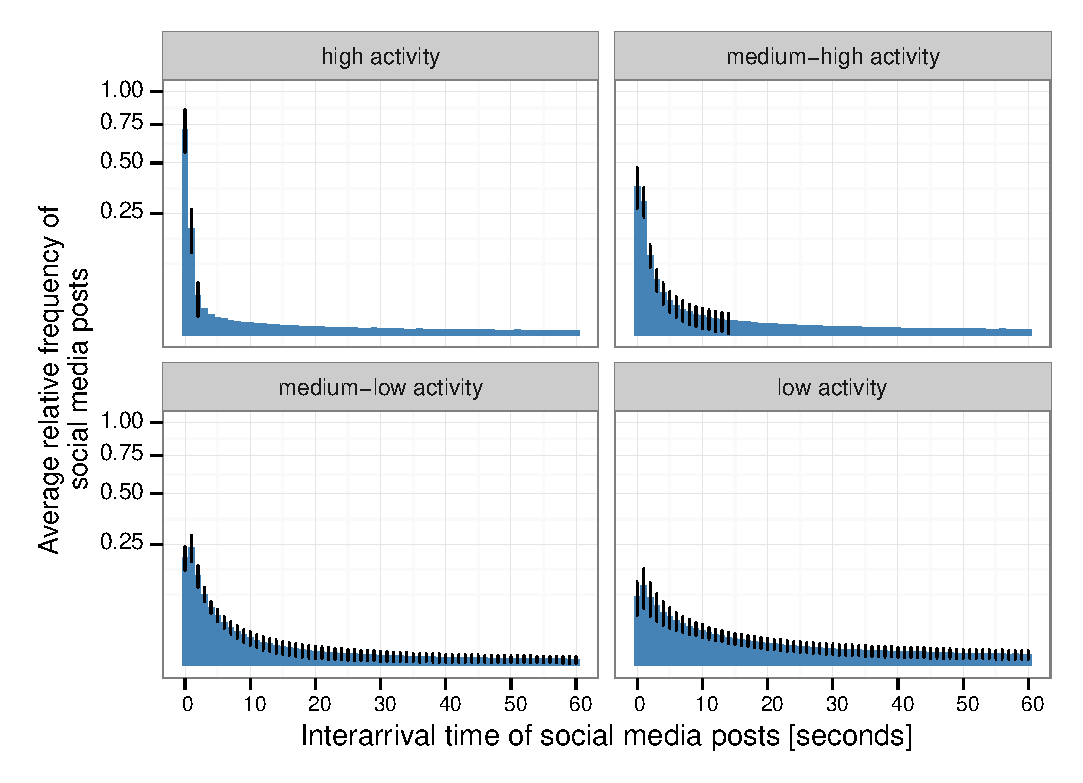
\includegraphics[width=\textwidth]{figures/high-activity/fig4}
  \caption[Average histograms of activity levels]{Average histograms of the high
      activity, medium-high activity, medium-low activity and low activity
      clusters in our dataset (from left to right and top to bottom). All
      histograms include standard deviation bars and were cut-off at 60 second
      length for better visibility.
      % \inote{change labels of x and y axis}
    }\label{fig:hi:avg-hist}
\end{figure}

Figure~\ref{fig:hi:avg-hist} shows the average histograms for events that belong
to the high activity, medium-high activity, medium-low activity and low-activity
clusters (displayed from left to right and top to bottom). 
%
All histograms show a quick decay in average relative frequency (resembling a
distribution from the exponential family). 
%
In particular, the high-activity group concentrates most of its activity in the
shortest inter-arrival rate, with lower activity groups mostly concentrating
their activity in the second bin with slower decay. 
%
Figure~\ref{fig:hi:scatter} further characterizes the differences in behavior of
the high and low-activity groups, showing that high-activity events concentrate
on average $70\%$ of their activity in the smallest bin ($0$ sec.), versus
$8\%$ for low-activity events. 
%
In addition, Figure~\ref{fig:hi:cdf} (left) shows the cumulative distribution
function (CDF) for each group of events, and Figure~\ref{fig:hi:cdf} (right)
shows $\log{(1 - \mathrm{CDF})}$. 
%
Visual inspection shows a clear difference in how inter-arrival rates are
distributed within each group, however, these figures do not indicate a
power-law distribution nor exponential distribution.%%

\begin{figure}[!htb]
  \centering
    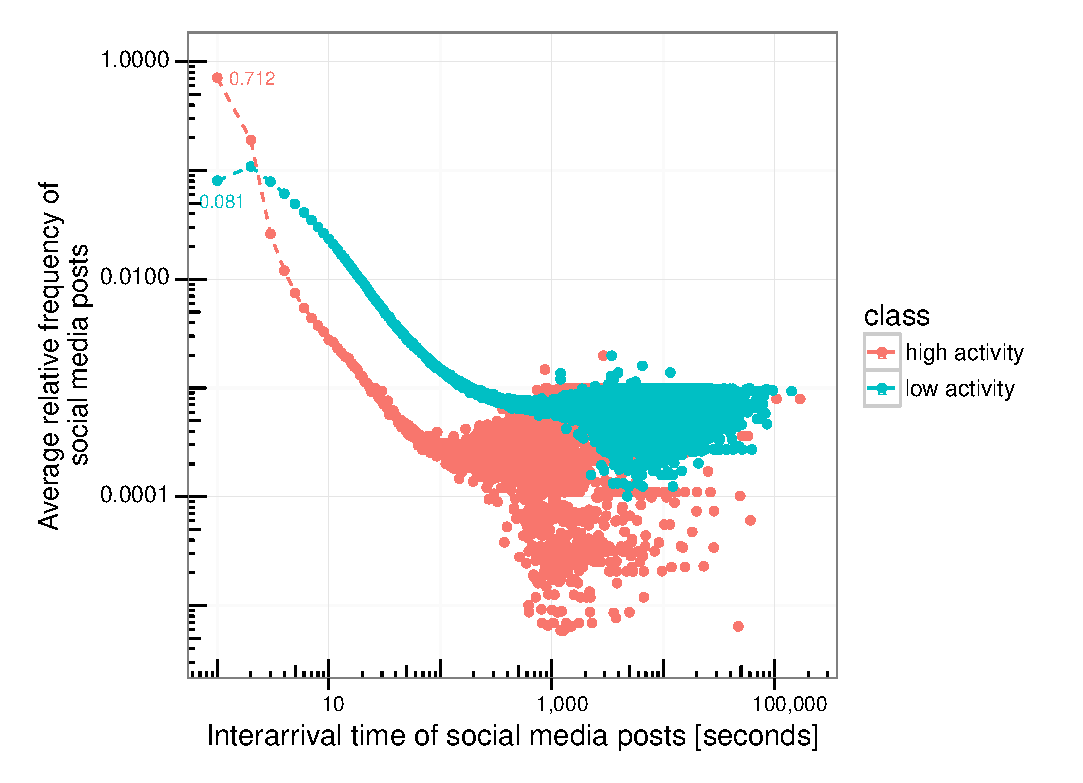
\includegraphics[width=\textwidth]{figures/high-activity/fig5}
  \caption[Relative frequencies of inter-arrival times]{Scatter plots of the
average relative frequencies of inter-arrival times for the high-activity and
low-activity clusters of events (i.e., scatter plots of the histograms in
Figure~\ref{fig:hi:avg-hist} in log-log scale). $y$-axis represents the average
relative frequency of social media messages and $x$-axis the inter-arrival time.}
\label{fig:hi:scatter}
\end{figure}

\begin{figure}
  \centering
  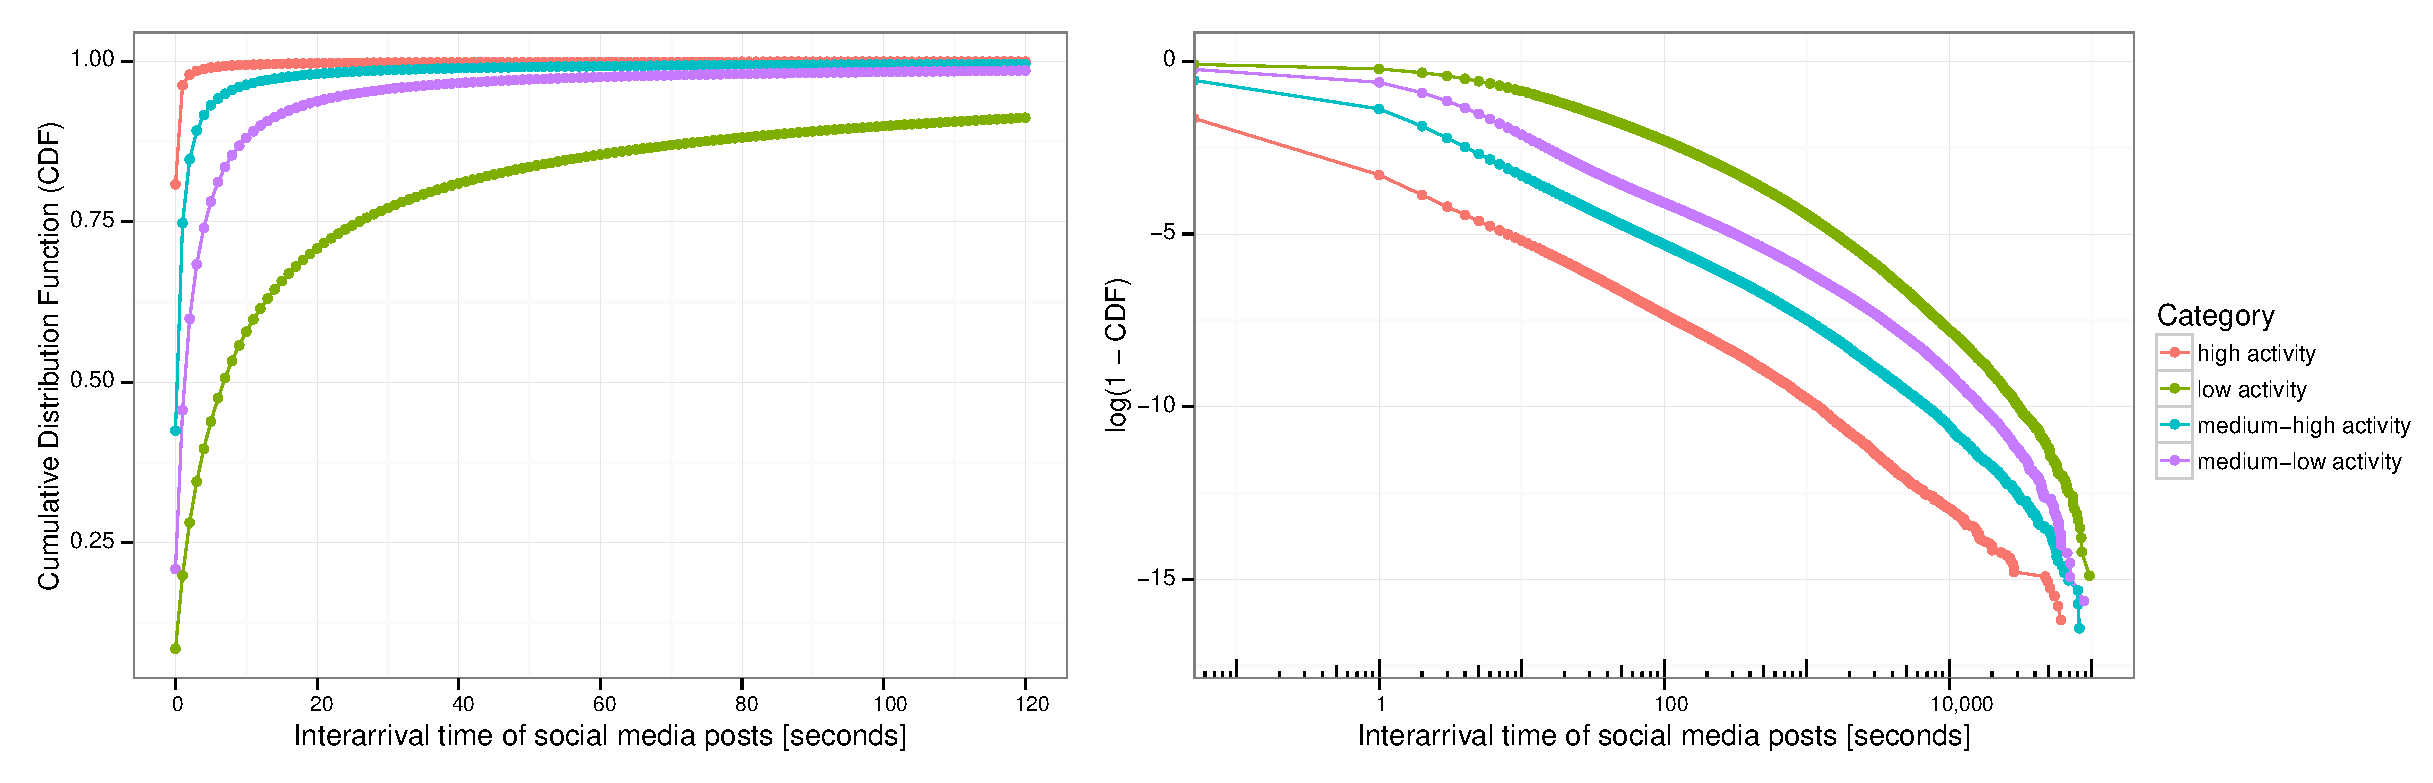
\includegraphics[width=\textwidth]{figures/high-activity/fig6_log}
  \caption[Cumulative Distribution Functions of activity levels]{{(Left) Average
cumulative distribution function (CDF) for the high activity, medium-high
activity, medium-low activity and low activity clusters in our dataset. (Right)
$\log{(1 - \mathrm{CDF})}$ for the same clusters. 
      % \inote{change labels of x and y axis}
    }}\label{fig:hi:cdf} %% fig6_long_inf_omitted.pdf
\end{figure}



Further analysis of the high-activity events shows significant differences to
other events, in the following aspects: 
%
(i) how the information about these events is propagated, 
%
(ii) the characteristics of the conversations that they generate, and 
%
(iii) how focused users are on the news topic. 

\subsection{Information Forwarding Characteristics}
\label{subsec:info_forwarding}

We found that high-activity events possess more information forwarding
characteristics than other events. 
%
We present four features which support this argument. 
%
The features, their description and their values are listed in
Table~\ref{tab:information_forwarding}.

The \texttt{retweet\_count} is generally higher for high-activity events.
%
This feature is the fraction of retweets present in the event, log-normalized by
the total amount of tweets in the event. 
%
A higher value suggests that people have a greater tendency to spread the
occurrence of these events, and forward this information to their followers. 

The \texttt{tweets\_retweeted} is lower for high-activity events than for the
rest. 
%
This feature is the number of tweets which have been retweeted, log-normalized
by the total number of tweets in the event. 
%
This suggests that the high amount of retweets for the high-activity events
actually originates from fewer tweets. This suggests that fewer tweets become
popular and are retweeted several times.

The \texttt{retweets\_most\_retweeted} is the total number of retweets of the
tweet that has been retweeted the most. 
%
This number is much higher for high-activity events than for low-activity
events, suggesting that the most popular tweet indeed becomes very popular when
the event is of high-impact.

\begin{table}
  \centering
  {\small
    \begin{tabular}{llll}
      \toprule
      Feature Name &  \multicolumn{1}{l}{Description} & high-activity, others& Hypothesis, $p$-value\\
      \midrule
      \texttt{retweet\_count} & \pbox{20cm}{$\log($total retweet count \\in the event divided by\\ total tweets in the event$)$} & $2.205, 1.473$ & $1$, $p = 0$ \\
      \midrule
      \texttt{tweets\_retweeted} & \pbox{20cm}{$\log($number of tweets \\retweeted divided by\\ total tweets in the event$)$} & $-1.091, -0.964$ & $1$, $p = 2.7\times10^{-5}$ \\
      \midrule
      \texttt{retweets\_most\_retweeted} & \pbox{20cm}{number of tweets of the\\ most retweeted tweet} & $284.491, 40.261$ & $1$, $p = 0$ \\
      \bottomrule
    \end{tabular}
  }
  \caption[Information forwarding characteristics of events]{Features which characterize the information forwarding aspect of an event.
  In general, high-activity events tend to have higher values for information forwarding 
  features than other events.}
  \label{tab:information_forwarding}
\end{table}

%%

In summary, high-activity events have a higher fraction of {\em retweets} (or
shares) relative to their overall message volume. 
%
On average, a tweet from a high-activity event is retweeted 2.36 times more than
a tweet from a low activity event. 
%
The most retweeted message in high-activity events is retweeted 7 times more
than the most retweeted message in a medium or low activity event. 
%
We find that a small set of initial social media posts are propagated quickly
and extensively through the network without any rephrasing by the user (just
plain forwarding). 
%
Intuitively, this seems justified given general topic urgency of high-activity
events. 
%
Events that are not high-activity did not exhibit these characteristics.

% %%


\subsection{Conversational Characteristics}
\label{subsec:conversational}

We found that high-activity events in general tend to generate more conversation
between users than the events in other categories. 
%
We observe this behavior through several features (Table~\ref{tab:conversational}).

\begin{table}
  \centering
  {\small
    \begin{tabular}{llll}
      \toprule
      Feature Name &  \multicolumn{1}{l}{Description} & high-activity, others & Hypothesis, $p$-value\\
      \midrule
      \texttt{replies} & \pbox{20cm}{$\log($total replies divided by\\ total tweets$)$} & $-1.4016, -1.6474$ & $1$, $p = 10^{-4}$ \\
      \midrule
      \texttt{norm\_replies} & \pbox{20cm}{$\log($number of replies divided\\ by total number of\\ unique users$)$} & $-1.5796, -1.9294$ & $1$, $p = 6.7\times10^{-4}$ \\
      \midrule
      \texttt{tweets\_replied} & \pbox{20cm}{$\log($number of tweets which\\ generated replies divided by\\ total tweets$)$} & $-1.7784, -2.0668$ & $1$, $p = 0.001$ \\
      \midrule
      \texttt{uniq\_users\_replied} & \pbox{20cm}{$\log($unique users who have\\ written a reply divided by\\ total tweets$)$} & $-1.7524, -2.0352$ & $1$, $p = 0.001$ \\
      \bottomrule
    \end{tabular}
  } \caption[Conversational features of events]{Features which characterize the
  conversational aspect of high-activity and remaining events. We argue that
  high-activity events tend to invoke more conversation among users than their
  counterparts.}
  \label{tab:conversational}
\end{table}

The features \texttt{replies} and \texttt{norm\_replies} both count the number
of replies, but have been normalized slightly differently. 
%
Both have a higher value for high-activity events suggesting that high-activity
events in general tend to spark more conversation between the users. 
%
The \texttt{tweets\_replied} feature counts the number of tweets which have
generated replies (it has been log-normalized by the total number of tweets in
the event). 
%
This is also higher for high-activity indicating that such events on average
have more tweets which invoke a reply from people. 
%
The \texttt{uniq\_users\_replied} feature counts the number of unique users who
have participated in an conversation. 
%
Again, this number is found to be higher for high-activity events than for
others suggesting that more users tend to engage in a conversation about these
events. 
%
All these features collectively suggest that high-activity events tend to have a
\emph{conversational characteristic} associated with them.

%%

In summary, high-activity events tend to spark more conversation between users,
33.4\% more than other events. 
%
This is reflected in the number of {\em replies} to social media posts. 
%
The number of different users that engage with high-activity events is 32.7\%
higher than in events that are not high-activity. 



\subsection{Topical Focus Characteristics}
\label{subsec:topical_focus}


We find that high-activity events have a lot more focus in terms of the topical
content than the remaining events. 
%
This possibly suggests that when a news item is sensational, people seldom
deviate from the topic of the news to other things. 

We used four features listed in Table~\ref{tab:topical_focus} to study the topic
focus characteristics of high-impact events.

\begin{table}
  \centering
  {\small
    \begin{tabular}{llll}
      \toprule
      Feature Name &  \multicolumn{1}{l}{Description} & high-activity, others & Hypothesis, $p$-value\\
      \midrule
      \texttt{uniq\_words} & \pbox{20cm}{$\log($total unique words \\divided by total tweets$)$} & $-0.1982, 0.1651$ & $1$, $p = 0$ \\
      \midrule
      \texttt{uniq\_chars} & \pbox{20cm}{$\log($total unique characters \\divided by total tweets$)$} & $2.0009, 2.0456$ & $1$, $p = 0$ \\
      \midrule
      \texttt{uniq\_hashtags} & \pbox{20cm}{$\log($number of unique hashtags\\ divided by total tweets$)$} & $-1.1126, 0.8761$ & $1$, $p = 0$ \\
      \midrule
      \texttt{uniq\_urls} & \pbox{20cm}{$\log($number of unique urls \\divided by total tweets$)$} & $-0.7194, -0.4951$ & $1$, $p = 0$ \\
      \bottomrule
    \end{tabular}
  } \caption[Topical focus features of events]{Features that were used to study
  the topical focus characteristics of high-activity events.}
  \label{tab:topical_focus}
\end{table}

The number of unique words (\texttt{uniq\_words}) and characters
(\texttt{uniq\_chars}) for high-activity events is lower than the remaining
events suggesting that the information content for high-activity events is more
focused than for the remaining events (as they do not need a diverse
vocabulary). 
%
Hashtags on Twitter are a sequence of characters that follow the \# symbol.
%
Conventionally, their purpose is to indicate the topic of the tweet. 
%
Again, this number (\texttt{uniq\_hashtags}, log-normalized by the total number
of tweets) is lower for the high-activity events than for the remaining events.
%
The number of unique URLs (\texttt{uniq\_urls}, which can be taken to interpret
similar semantics as the hashtags) is also lower for high-activity events than
for the rest. 


%%

Summarizing, posts about high-activity events are much more topic focused than
in other events. 
%
The vocabulary of unique words as well as {\em hashtags} used in high-activity
events is much more narrow than for other events. 
%
Medium and low activity events have over 7 times more unique hashtags than
high-activity events. 
%
This is intuitive, given that if a news item is sensational, people will seldom
deviate from the main conversation topic.

%%

\subsection{Predicting the Activity of Events}

In a real-world scenario, in order to predict if an early breaking news story
will have a considerable impact in the social network, we will not have enough
data to create its activity-based model, i.e., we will not yet know the
distribution of the speed at which the social media posts will arrive for the
event. 
%
For instance, an event can start slowly and later produce an explosive reaction,
or start explosively and decay quickly to an overall slower message arrival
rate. 
%
Still, reliable early prediction of very high-activity news is important in many
aspects, from decisions of mass media information coverage, to natural disaster
management, brand and political image monitoring, and so on.

%%

For the task of early prediction of high-activity events we use features that
are independent of our activity-based model such as the retweets, the sentiment
of the posts about the event, etc. These features are computed on the early 5\%
of messages about the event.
%
A list of all the features used for classification is shown in Table
\ref{tab:feats}.
%
The results are an average from a 5-fold cross validation with randomly selected
60\% training, 20\% validation and 20\% test splits.
%
The classification was carried out using logistic regression provided by the Weka
package.
%
The high-activity events are identified with a precision of 82\% using only the
earliest 5\% of the data of each event (Table~\ref{tab:classification_results}).
%
Additionally, we were able to identify with high accuracy a considerable
percentage of all high-activity events ($\approx 46\%$) at an early stage, with
very few false positives (Table~\ref{tab:classification_results}
and~\ref{tab:confusion_matrix}).

\begin{table}
  %\begin{adjustwidth}{-10mm}{-10mm}
  \centering
  {\small
    \begin{tabularx}{\textwidth}{lcccc|cccc}
      \toprule
      & \multicolumn{4}{c}{\textbf{Early 5\% Tweets}} & \multicolumn{4}{c}{\textbf{All Tweets}} \\
      \midrule
      & FP-Rate & $P$ & $R$ & ROC-area & FP-Rate & $P$ & $R$ & ROC-area \\
      % \midrule
      high-activity & 0.009 & 0.819 & 0.455 & 0.900 & 0.01 & 0.830 & 0.540 & 0.945 \\
      non-high-activity & 0.545 & 0.954 & 0.991 & 0.900 &  0.460 & 0.960 & 0.990 & 0.945 \\
      \bottomrule
    \end{tabularx}
  }
  \caption{{Classification results of high-activity events.}}
  \label{tab:classification_results}
  %\end{adjustwidth}
%                                                                                                                                448,1         93%
\end{table}

\begin{table}
  \centering
  % {\scriptsize
  \begin{tabularx}{\textwidth}{lcc|cc}
    \toprule
    \multirow{2}{*}{ }& \multicolumn{2}{c}{\textbf{Early 5\% Tweets}} & \multicolumn{2}{c}{\textbf{All Tweets}} \\
    \midrule
    % \cmidrule{2-5} \cline{2-5}
    & high-activity & non-high-activity & high-activity & non-high-activity \\
    % \midrule
    high-activity & $194$ & $232$ & $230$ & $196$\\
    non-high-activity & $43$ & 4,765 & 47 & 4,761 \\
    \bottomrule
  \end{tabularx}
  % }
  \caption{{Confusion matrix for high-activity events prediction.}}
  \label{tab:confusion_matrix}
\end{table}



The precision using only the early tweets is almost as good as using all tweets
in the event (0.819 to 0.830). 
%
This suggests that the social network somehow acts as a natural filter in
separating out the high-activity events fairly early on.  
%
The recall goes from 0.455 to 0.540. 
%
This indicates that there are some high-activity events which require more data
in order to determine what kind of activity they will produce, or events for
which activity occurs due to random conditions. 



{\footnotesize
  \begin{longtable}{l|l|l}

    \hline \textbf{Feature Name} & \textbf{Normalized By} &
    \textbf{Normalization
      Method} \\
    \hline
    \endfirsthead
    \multicolumn{3}{l}%
    {\tablename\ \thetable\ -- \textit{Continued from previous page}} \\
    \hline \textbf{Feature Name} & \textbf{Normalized By} &
    \textbf{Normalization
      Method} \\
    \hline
    \endhead
    \hline \multicolumn{3}{l}{\textit{Continued on next page}} \\
    \endfoot
    \hline
    \endlastfoot


    \texttt{component\_size}	&	 None	&	  \\
    \texttt{total\_seconds}	&	 \texttt{total\_tweets}	& $\log(x) - \log(y)$ \\
    \texttt{total\_tweets}	&	 None	&	  \\
    \texttt{total\_retweets}	&	 \texttt{total\_tweets}	&	 $\log(x) - \log(y)$ \\
    \texttt{total\_tweets\_retweeted}	&	 \texttt{total\_tweets}	&	 $\log(x) - \log(y)$ \\
    \texttt{retweets\_most\_retweeted}	&	 \texttt{total\_retweets}	&	 $\log(x) - \log(y)$ \\
    \texttt{total\_mentions}	&	 \texttt{total\_tweets}	&	 $\log(x) - \log(y)$ \\
    \texttt{total\_unique\_mentions} &
    \texttt{total\_mentions}	&	 $\log(x) - \log(y)$ \\
    \texttt{total\_tweets\_with\_mention}	&	 \texttt{total\_tweets}	&	 $\log(x) - \log(y)$ \\
    \texttt{total\_tweets\_with\_mostfrequent\_mention}	&	 \texttt{total\_tweets\_with\_mention}	&	 $\log(x) - \log(y)$ \\
    \texttt{total\_hashtags}	&	 \texttt{total\_tweets}	&	 $\log(x) - \log(y)$ \\
    \texttt{total\_unique\_hashtags}	&	 \texttt{total\_hashtags}	&	 $\log(x) - \log(y)$ \\
    \texttt{total\_tweets\_with\_hashtag}	&	 \texttt{total\_tweets}	&	 $\log(x) - \log(y)$ \\
    \texttt{total\_tweets\_with\_mostfrequent\_hashtag}	&	 \texttt{total\_tweets\_with\_hashtag}	&	 $\log(x) - \log(y)$ \\
    \texttt{total\_urls}	&	 \texttt{total\_tweets}	&	 $\log(x) - \log(y)$ \\
    \texttt{total\_unique\_urls}	&	 \texttt{total\_urls}	&	 $\log(x) - \log(y)$ \\
    \texttt{total\_tweets\_with\_url}	&	 \texttt{total\_tweets}	&	 $\log(x) - \log(y)$ \\
    \texttt{total\_tweets\_with\_mostfrequent\_url}	&	 \texttt{total\_tweets\_with\_url}	&	 $\log(x) - \log(y)$ \\
    \texttt{total\_unique\_verified\_users}	&	 \texttt{total\_verified\_users}	&	 $\log(x) - \log(y)$ \\
    \texttt{total\_verified\_users}	&	 \texttt{total\_tweets}	&	 $\log(x) - \log(y)$ \\
    \texttt{total\_unique\_users}	&	 \texttt{total\_tweets}	&	 $\log(x) - \log(y)$ \\
    \texttt{total\_replies} & \texttt{total\_unique\_users} &
    $\log(x) - \log(y)$ \\
    \texttt{total\_tweets\_first\_replied} & \texttt{total\_tweets} &
    $\log(x) - \log(y)$ \\
    \texttt{total\_unique\_users\_replied} &
    \texttt{total\_unique\_users} &
    $\log(x) - \log(y)$ \\
    \texttt{total\_tweets\_replied}	&	 \texttt{total\_tweets}	&	 $\log(x) - \log(y)$ \\
    \texttt{total\_words}	&	 \texttt{total\_tweets}	&	 $\log(x) - \log(y)$ \\
    \texttt{total\_unique\_words}	&	 \texttt{total\_words}	&	 $\log(x) - \log(y)$ \\
    \texttt{total\_characters}	&	 \texttt{total\_tweets}	&	 $\log(x) - \log(y)$ \\
    \texttt{total\_rt\_count}	&	 \texttt{total\_tweets}	&	 $\log(x) - \log(y)$ \\
    \texttt{total\_fav\_count}	&	 \texttt{total\_tweets}	&	 $\log(x) - \log(y)$ \\
    \texttt{total\_positive\_sentiment}	& \texttt{total\_tweets}	&	 $x / y$ \\
    \texttt{total\_negative\_sentiment}	&	 \texttt{total\_tweets}	&	 $x / y$ \\
    \hline

    \caption[Features used for classification of activity]{List of
        features used for characterization and classification. The
        ``Normalization Method'' column corresponds to the method used to
        normalize the value of the first column using the value of the second
        column. For example, the total number of retweets was normalized
        dividing it by the total number of tweets, and then taking the
        logarithm. Zero values were replaced by $10^{-8}$.}
    \label{tab:feats}
  \end{longtable}}



\section*{Conclusion}

We show that there are several properties that separate how
high-impact news events evolve in Twitter in comparison to other
events. We have created a model for events that allows us to do
unambiguous classification of high-impact events based on their impact
in the social network, in terms of the distribution of their
inter-message arrival rates. This definition does not have some of the
problems that current notions of virality and popularity have. Some
characteristics of high-impact events are that they are forwarded more
often by users, and generate a greater amount of conversation than
other events.  Social media posts from high-impact news events are
much more focused on the news topic. Our experiments show that there
are several properties that can suggest early on if an event will have
high-impact on the on-line community.  We can predict a high number of
high-impact events {\em before} the network has shown any type of
explosive reaction to them. % Using simple off-the-shelf feature based
classifiers, we can
% predict many high-impact events with high precision.
This suggests that users are collectively quick at deciding whether an
event is important or not.  However, there does exist a fraction of
events which will become high impact, despite not presenting
patterns of other high impact events during their early stages.  These
events are likely to be affected by other factors, such as random
conditions found in the social network at the moment and require
further investigation.
\chapter{Spatio-Temporal Context: Inferring Geopolitical Interactions on Twitter}
\chapter{Aggregating Content: A Lightweight Model of News Events}
\label{chapter:url}

\section*{Abstract}
  The sheer amount of newsworthy information published by users in social media
  platforms makes it necessary to have efficient and effective methods to filter
  and organize content. 
  %
  In this scenario, off-the-shelf methods fail to process large amounts of data,
  which is usually approached by adding more computational resources. 
  %
  Simple data aggregations can help to cope with space and time constraints,
  while at the same time improve the effectiveness of certain applications, such
  as topic detection or summarization. 


  %
  We propose a lightweight representation of newsworthy social media data. 
  %
  The proposed representation leverages microblog features, such as redundancy
  and re-sharing capabilities, by using surrogate texts from shared URLs and word embeddings.
  %
  Our representation allows us to achieve comparable clustering results to 
  those obtained by using the complete data, while reducing running time and 
  required memory.
  %
  This is useful when dealing with noisy and raw user-generated social media data.

\section{Introduction}
\label{sec:introduction}

%\mq{hablar de multimodal summarization, diferentes tamaños de topicos, clustering incremental, 
%redundancia ayuda a word embeddings?, complejidad de otros metodos}

%%%%% Index
% Context
% Motivation
% Problem statement
% Contributions

%%%% Content


% Context 
% \subsection{context}

%Un modelo de "representacion" de informacion (de evento en SM) de manera compacta 
%para incorporar nuevo conocimiento.... con aplicaciones A, B y C

%Una forma de modelar la informacion .... (alto nivel)
%Describir semi-formalmente el modelo 
%Poder separar "señales" o "aspectos" del evento 

%Presentar casos de estudio que muestren las N aplicaciones. Mostrar ejemplos de 
%cada aplicacion.

%ej, aplicacion "event retrieval": dado un evento, identificar contenido relevante, topicos o aspectos
%relevantes al evento real (?) 

%modelo con WE exacerba diferencias en los documentos para separar topicos usando UCG (redundancia)

%hipotesis con respecto a agrupar por url: contenido relevante es mas probable de ser compartido con las mismas
%urls que contenido no relevante 


% Nowadays, social media platforms have become a main source of news. According to
% a recent survey, by 2018 about two thirds of US adults used social media as a
% source of news~\cite{pewresearch}, and about 70 percent of Twitter users get
% news from there. With their scale, popularity, and ease of use, social media
% platforms have drastically lowered the entry barriers to disseminate newsworthy
% information in real time. 
%Due to that, news events are often reported earlier in
%social media than in traditional news media. 

% In particular, impactful or breaking real world events (such as the 2015 Nepal
% Earthquake or the 2017 Brexit) overflow social media with millions of messages.
% For that reason, it is a hard task for humans to go through every message in
% order to understand what an event is about. 


The sheer amount of newsworthy information published by users in social media
platforms makes it necessary to have efficient and effective methods to filter
and organize content. 
%
In this scenario, off-the-shelf methods fail to process large amounts of data,
which is usually approached by adding more computational resources. 
%
Simple data aggregations can help to cope with space and time constraints,
while at the same time improve the effectiveness of certain applications, such
as topic detection or summarization. 


%
We propose a lightweight representation of newsworthy social media data. 
%
The proposed representation leverages microblog features, such as redundancy
and re-sharing capabilities, by using surrogate texts from shared URLs and word embeddings.
%
Our representation allows us to achieve comparable clustering results to 
those obtained by using the complete data, while reducing running time and 
required memory.
%
This is useful when dealing with noisy and raw user-generated social media data.


The overload of information in social media streams makes it difficult for users
to obtain a comprehensive account of different emerging events reported by
users.
%
%to get a complete picture of an event or find relevant messages.
%
The ability to identify and summarize relevant information about newsworthy
topics that are accounted for by users in social media can be of great use to
society.
%
This is particularly true in the case of high impact and breaking news, like
natural disasters and crisis situations~\cite{ICWSM1817816}.
%\bp{agregar mas citas}.
%
In general, social media platforms present their content to the consumer in one
of two ways: (1) by displaying user posts in reverse chronological order, or (2)
by displaying posts in a personalized fashion, showing first what they deem more
interesting to the user.
%
However, if the user 
%consuming social media content 
is seeking information about a specific event, the aforementioned approaches can
result also in unnecessary exposure to redundant, irrelevant, or even misleading
information.
%
In this context, delivery of key pieces of information to the user is important,
and even critical in some cases; 
%
for instance, social media is often used as a complementary source of
information for disaster management and
response~\cite{ICWSM1817816,Sarmiento:2018:DDE:3201064.3201077}
%\bp{agregar citas}
and also to obtain information about newsworthy events not yet reported by
formal news outlets. 
%
%In this sense, thThis need to produce high-quality real-time information requires effective ways to filter and organize information about real-world events on social media.
%

Despite the usefulness of social media as a worldwide news information source,
its consumption is not without challenges.
%
These challenges include, among many others, correctly assessing information
veracity and relevance to a specific topic, as well as dealing with a huge
volume of data with variable quality. 
%
%In this sense, the consumption of social media content for information seeking about particular events requires effective ways to filter and organize streaming data.
%%
%
%Specifically, the task of organizing and filtering
%
%Filtering and organizing information in social media can be a
%particularly challenging task.
%
In particular, we study Twitter, in which users can post text-based messages.
%
These messages, called {\em tweets} can include links to images, videos, to
external web-pages or to other tweets, making this platform's content multimodal.

%
%From the perspective of understanding current events, tweets contain a large volume of irrelevant and redundant content, which can often be misspelled, or unreliably capitalized, 
%
%On the other hand, we observe several 
The URLs shared in Twitter often link to varied types of media (articles,
images, or videos), which have been found useful for identifying conversation
topics~\cite{mishne2012twanchor}.
%
In the context of news events, users tend to quickly re-share information if the
event sparks high interest (see Section~\ref{subsec:info_forwarding}), which
results in many (near-)duplicate messages.
%
Dealing with content of these characteristics requires different approaches
than with traditional media~\cite{Alonso:2017:WHH:3091478.3091484}.
%
Prior work has acknowledged the need of techniques for dealing with this type of
social media data.



%%


In this work we focus on the problem of producing summarized representations of
social media data related to news events without significant loss of
information.
%
We present a compact representation for social media content related to news
events.
%
This representation allows us to preserve information about the topics involved
in an event, and to identify relevant content, while reducing the volume of
data.
%
This can be especially useful for online data processing about developing news
and news information seeking tasks.
%
To achieve this, our model annotates shared URLs with the text of the messages
in which they appear.
%
Here we use messages as {\em anchor text} or {\em surrogate text}. 
%
We first leverage this idea by identifying relevant URLs that are shared in
social media during a news event.
%
We discard URLs that are too general with respect to an event (e.g. a general
report), or generic (e.g. linking to the homepage of a news outlet) as we deemed
them as non-relevant.
%
Then we aggregate all the anchor texts associated with relevant URLs into {\em
documents}, and all the conversations around those documents as well. 

As a preliminary way to study the usefulness of our event representation, we
applied it to three news events as a case study.
%
We observed that our representation reduces the amount of records needed to
describe an event by one order of magnitude, compared to using the raw tweets. 
%
We were also able to identify sub-topics by clustering the documents using dense
word representations, such as neural network--based word embeddings. 
%
We show that the clustering based sub-topic detection task using our proposed
representation yields similar external quality metrics to those obtained using
the entire data. 
%
Hence, indicating that we are preserving relevant aspects of the information
while considerably reducing running time.

\paragraph{Contributions.} Our contributions in this chapter are the following:

\begin{enumerate}
  \item We present a novel compact representation for news event information in
  microblogs, based on shared URLs. This representation reduces data volume.

  \item We study the usefulness of our representation through three case
  studies. We do so by introducing a methodology to represent news events in
  Twitter and find sub-topics. We show that our approach displays comparable
  performance to baseline methods at a fraction of the computational resources.
\end{enumerate}


% problemas con representar social media content
% Representing content generally involves representing its constituent terms in
% another space. For instance, using weighted term frequency vectors, graph
% models, or probabilistic models over the distribution of terms. In social media,
% these methods result in highly dimensional sparse features, which are difficult
% to manage without large quantities of well-curated messages. On the other hand,
% it is not trivial to manage large scale data. Current methods can manage large
% volumes of messages at great computational expense or by splitting the dataset
% in smaller sets and dealing with them separately. For example, traditional ways
% of representation of text, such as term frequency weighting, involves the
% generation of thousands of dimensions on messages that are about 10 to 20 words
% long.

% Nonetheless, in the context of news events, user-generated content can be leveraged
% to estimate the relevance of the information and to annotate content from
% external sources. We start from the assumption that users share and comment on
% content that is relevant or interesting to them. Hence, the existence of several
% messages on a topic suggests that the topic is important to users. We can
% leverage this idea even futher: we can annotate the shared URLs in user posts
% with the same text that users put in the posts that contains those URLs. In the
% literature, the text that accompanies a URL is usually known as {\em anchor text}, or
%   {\em surrogate text}, and this idea has been extensively used in query log
% mining~\cite{Beeferman:2000:ACS:347090.347176,10.1007/978-3-540-30192-9_58}. We
% can also take advantage of the redundancy of posts in social media. When exposed
% to an emergent news, users tend to share information as quickly as
% possible~\cite{kalyanam2016prediction}, and this often results in duplicate and
% near-duplicate data. This information can be useful to assess the
% importance of certain aspects of the event. In this work, we exploit these clues
% in order to design a model to represent newsworthy information.

% reescribir
% We propose a lightweight representation of news events in Twitter by aggregating
% tweets based on the existence of shared URLs. Our representation groups tweets
% by common shared URLs into {\it components}, and also ignoring highly common
% URLs in the dataset, in order to avoid having large components of unrelated
% tweets. This representation reduces the amount of records to be processed by one
% order of magnitude, and we validate its capabilities by performing clustering on
% three selected news events to identify sub-topics. By using dense
% representations of words, such as neural network based word embeddings, our
% model generates a compact representation of news events. We show that we achieve
% similar performance on sub-topic detection at a fraction of the time and memory
% required. Our proposed representation allows us to process raw, un-curated
% Twitter data faster than with using individual tweets, and it is flexible enough
% to incorporate new data as the event evolves in time.

% We propose a simple model to represent information about news events in Twitter
% using aggregations of tweets that mention the same URLs, and that retweet or
% reply themselves. Then, we model the resulting sets of documents using dense
% vector representation of terms, such as neural word embeddings, using a corpus
% of 193 million news-related tweets. With this representation, we exploit
% features often discarded in similar works, such as repeated messages and URLs
% mentioned in tweets. This results in a smaller and more flexible representation,
% which allows us to perform some tasks more efficiently, and to incorporate new
% information to the model with little effort. Our event representation is
% compatible with current approaches regarding Twitter event data, such as event
% detection, filtering, and summarization. We show the effectiveness of this
% representation by characterizing topics in news events shared in Twitter, which
% can contain several repeated or irrelevant posts. The topics consist of diverse
% tweets that share URLs, which can be seen as a multimedia representation of
% topics, regardless of the content of these URLs (images, videos, news articles,
% etc.). 




% problemas: mucha info, redundante, etc. 
% explotamos eso para mejorar la origanizacion de la info
% mostramos que es util para: ...
% tiene estas caracteristicas: ...


% One particular problem is what is called information overload: when users are
% exposed to way more information than they can process and understand, and
% effective methods to find relevant information are missing, assuming that
% users know what they are looking for. In this context, automatic summarization
% was proposed as a way to tackle this problem. Given a document or a set of
% documents about a specific topic, the output of the summarization method is a
% gist that summarizes the content, under certain criteria and restrictions. 


% In this work, we approach the issue of information overload by modeling
% content associated with online news, as propagated on Twitter. 
% When a {\em breaking news} occur, users tend to share and
% forward information about it as quickly as possible {\bf REF PLOS}, and ...

% motivation
% \subsection{motivation} 
% user contributed content reflect opinions of users, not media
% importance given by users
% free annotations of urls 




% problems with social media
% \subsection{challenges}
% events are noisy (different levels of relevance)


% However, the scale and rate of publication makes it difficult to understand
% what is happening or what an event is about. Also, the presence of irrelevant
% posts makes it even more difficult to understand a specific event. Usually,
% when a user wants to know about a certain ocurrence, he or she performs a
% search using some keywords, and a chronologically ordered timeline of the most
% recent posts is then shown. In other cases, a special sorting is made in order
% to show the most relevant posts that specific user might like the most, or
% just the posts with the highest scores in terms of popularity. However, this
% is not enough to understand the different aspects or topics related to an
% event.

% Different approaches have been proposed to help users understand the content.
% For example, automatic text summarization is used in order to select the most
% salient phrases from a set of documents, aiming for optimizing diverse criteria,
% such as relevance, coverage, or popularity. However, nowadays online news media
% has increasingly shifted their focus towards multimedia content {insertar
% cita}. There have been some efforts in order to summarize content of different
% modalities, such as images or videos in isolation, but few consider a mixture of
% them. Our hypothesis is that a summary in different content modalities, such as
% images, videos, and text, is more effective than a text-only, or images-only
% summary in order to understand an event. In other words, our hypothesis is that
% a multimodal summary is more informative than a unimodal one. In this work, we
% discuss the challenges of the current approaches and tackle the problem of
% multimedia summarization of events in social media, by considering content
% independently of its nature.



% problem statement
% \subsection{problem statement}

% hypotheses
% \subsection{hypotheses}
% Hypotheses: 
% 1. grouping tweets by url improve the ...
% 2. the use of word embeddings (fasttext) improve the ...

% % contributions
% % \subsection{contributions}
% Our contributions are the following:
% \begin{enumerate}
%   \item We investigate 
%   \item
%   \item ?
% \end{enumerate}


% % outline of paper
% % \subsection{outline}
% This paper is organized as follows. Section ...

% % -----------------------------------------------------------------------

% % Twitter desc
% On Twitter, each post, called {\em tweet}, is a short text ---traditionally
% 140 characters long, but by the year of 2017 this limit was extended to 280
% characters---, which can contain arbitrary URLs, as well as {\em hashtags}
% (words prepended with a \#, serving to the tweet as tags), {\em cashtags}
% (prepended by a \$, serving as identifiers for stocks and shares), and mentions
% (names of Twitter users).

\section{Related Work}\label{sec:related}
% There is extensive work on automatic summarization on microblogs\mq{ref}. In
% this work, we approach the problem from a practical point of view, where our
% goal is to benefit from the characteristics of social media posts, in
% particular, from event-related messages. We exploit the redundancy of
% information available in social media via the aggregation of information
% around shared URLs, and propose a simple and compact model using word
% embeddings on tweets. Therefore, we can classify the related work in three
% areas: modeling social media content, automatic summarization of news, and
% usage of word embeddings in social media.

Two lines of research are relevant to our work: the utility of anchor texts in
microblogs and topic detection methods using different aggregation strategies. 

%\bp{No hay literatura de representaciones compactas de eventos para sumarizacion?}


%%%%% Studies from 201x have shown that around 25\% of tweets contain at least one URL.
There have been studies about the usefulness of anchor texts in Twitter. 
%
Raux et al.~\cite{raux2011describing} used anchor texts from tweets pointing to a
predefined set of URLs to characterize general topics, by clustering a bipartite
graph of words and URLs. 
%
We instead focus on news events, and tweets related to these news, without using
predefined URLs, but instead the actual shared URLs. 
%
Mishne and Lin~\cite{mishne2012twanchor} studied the
contribution of anchor texts compared to the text of the websites behind the
URLs, concluding that anchor text add new terms not seen in the website content,
by looking also at the conversations around the sharing tweets. 
%
Alonso et al.~\cite{Alonso:2015:WCW:2740908.2745397} had similar findings examining
Facebook posts. 
%
In another work by Alonso et al.~\cite{Alonso:2017:WHH:3091478.3091484}, the authors designed a social search
engine using the propagation of shared URLs as cues to measure virality, and anchor texts to augment metadata of the search results with social
content. 
% In a previous work~\cite{quezada2013understanding}, we showed a
% prototype of a multimodal summarization methodology using anchor texts. In this
% work, we do not make use of or compare to the content of the URLs themselves,
% but use solely the anchor texts as a mean to represent the content about a news
% event.

Topic modeling of tweets is an active line of research, and there are some
studies which investigate the effectiveness of aggregation of tweets to improve
topic
detection~\cite{Hong:2010:EST:1964858.1964870,Mehrotra:2013:ILT:2484028.2484166,alvarez2016topic}.
Hong and Davison~\cite{Hong:2010:EST:1964858.1964870} analyzed the effects of
different aggregation strategies of tweets when finding topics with Latent
Dirichlet Allocation. They found that some schemes yield better results at some
tasks, such as classification problems related to tweets. In a similar fashion,
Mehrotra et al.~\cite{Mehrotra:2013:ILT:2484028.2484166} observed that
aggregating hashtags (also denoted as {\em pooling} of tweets by hashtags) is a
more effective strategy to identify topics from tweets, but at the cost of
longer running times due to the duplication of tweets. Finally, Alvarez-Melis
and Saveski~\cite{alvarez2016topic} found that adding the threads of
conversation into the pooling is more effective than pooling by hashtag in their
observations. We instead aggregate by shared URLs and conversations, yielding
similar performance to our baseline, with reduced running time.



% \subsection{Using common information in tweets}

% Similar to our work, in the sense of exploiting common information across
% messages, the work of Kamath et al.~\cite{Kamath:2013:SDO:2488388.2488447}
% focuses in the spatio-temporal dynamics of {\em memes}, as seen as units of
% information spreaded in social media. For this, they model each tweet as a
% tuple of the hashtags involved, time, and location to observe and characterize
% topics in Twitter. Similarly, the work of Pe\~na-Araya et
% al.~\cite{pena2017gaining} aim to characterize geopolitical entities (such as
% countries) based on the tweets that mention them, by proposing a model to
% represent locations in a spatio-temporal ambit, and develop a visual analytics
% tool to explore events based on the location scope of their impact. Our work
% is similar to both in the sense of leveraging common entities across messages,
% in this case, the URLs, in order to generate a compact representation to
% facilitate the discovering of sub-events. In our case, we do so by using URLs
% and the text content as a surrogate for the URLs, also called anchor texts.

% Concerning the specific use of anchor text in social media, Mishne and
% Lin~\cite{mishne2012twanchor} show that the anchor texts in general tweets
% provide additional new information compared to the content of webpages alone
% in a study of 7 million URLs obtained from the Twitter Firehose. The work of
% Raux et al.~\cite{raux2011describing} is one of the first to use anchor texts
% to find clusters of topics in Twitter, in order to describe Web content using
% tweets. The authors create a weighted bipartite graph of tweet words and URLs,
% being the weight the tf-idf score of the words in the tweets that contain the
% URL, and then find clusters of URLs. Although they characterize clusters of
% URLs as topics, their work focuses on general tweets and not newsworthy
% messages in particular. In the work of Alonso et
% al.~\cite{Alonso:2017:WHH:3091478.3091484}, the authors develop a search
% engine for content related to URLs shared on Twitter, displaying the most
% popular and viral URLs, also showing the effectiveness of this approach. In
% our previous work~\cite{quezada2013understanding}, we show a prototype of a
% automatic summarization methodology using tweets aggregated by URL, and then
% modeling the aggregated sets as tf-idf vectors to cluster them, find sub-events, 
% and then selecting the most representative messages as a multi-modal
% summary.

% % \subsection{General text representation methods}

% % % verificar
% % %In a general domain, LDA is very good to find/extract topics, but not in the 
% % %domain of this work. So my magnificent research is pretty very much fabulous.

% % Topic models are a useful way to deal with textual information and to derive a
% % low-dimensional representation of documents. One of the most popular methods
% % is Latent Dirichlet Allocation, or LDA~\cite{blei2003latent}. LDA models a
% % document as a mixture of different topics, which are probability distributions
% % on the vocabulary. TwitterLDA~\cite{zhao2011comparing} is a modification to the 
% % original approach, by changing the assumption that a single document can discuss different topics, which may be unlikely in short messages, such as tweets. Our representation is 
% % compatible with LDA or TwitterLDA, as it provides a way to aggregate topical information which can
% % be used as input for topic models.

% % We also use dense word embeddings such as the continuous representations obtained by using shallow
% % neural networks such as {\tt word2vec}~\cite{DBLP:journals/corr/abs-1301-3781} 
% % or {\tt fastText}~\cite{bojanowski2016enriching}. Dense vector representation of words
% % provide a efficient way to assess the similarity of terms or documents. In contrast,
% % traditional methods, such as tf-idf~\cite{Salton:1983:EBI:182.358466}, involve generating embedding of words of thousands of dimensions, as high as the vocabulary size. Some methods, such as
% % Latent Semantic Analysis~\cite{dumais2004latent}, aims to reduce the dimensionality of the representation by doing matrix factorization. In our case, our model aims to generate a representation of low dimensionality by using neural word embeddings over the aggregation of 
% % related messages, and by doing so, reducing the amount of documents.


% \subsection{Applications of tweet representations}

% Automatic text summarization has been employed in different domains, such as
% news~\mq{cite}, sports~\cite{meladianos2018optimization,chakrabarti2011event},
% music~\cite{raposo2016using}, or movies~\cite{aparicio2016summarization}.

% There are several approaches for automatic summarization of events from social
% media, being many of them inspired in automatic text summarization. In order
% to manage scale, most of the related approaches do not deal with all the data
% at once, but work with similar sub-problems, such as sub-events detected via
% time windows, clustering, or online approaches. 

% The work of Chakrabarti and Punera~\cite{chakrabarti2011event} identifies
% particular time windows in structure-rich events, such as football matches.
% Using Hidden Markov Models, the authors find time windows associated with
% specific sub-events (e.g., a "touchdown") and then summarize each sub-event
% using a centroid-based approach on the tf-idf representation of the tweets.
% Similarly, Alsaedi et al.~\cite{alsaedi2016temporal} fix a time window of one
% hour to define all the tweets in that time window as a cluster, and then use
% two consecutive clusters to take into account the changes between time
% windows. They also propose two additional approaches, namely using a retweet
% voting approach and a temporal centroid method. In all cases, the approaches
% do not use all the dataset at once, but select a limited amount of messages as
% a sub-event. 

% We do not follow this approach, mainly because different sub-events  
% may be mentioned in different stages of the event, and the time-window
% approach can result in low purity clusters when being applied to general
% events.


% One of the first online approaches to event detection and summarization in
% Twitter is the work of Sankaranarayanan et
% al.~\cite{Sankaranarayanan:2009:TNT:1653771.1653781}. The authors describe a
% system that collects tweets and identifies events using an online clustering
% procedure over a tf-idf representation of tweets. \mq{problema con esto}




% \mq{completar (eval)} There is no definitive standard against which one can
% compare the results from an automated summarization system. In general, the
% methods for evaluating summaries can be classified in two kinds: intrinsic or
% extrinsic. The first one evaluate the quality of the summary itself, e.g.,
% compare the summary generated by the system with other summaries generated by
% human experts, whereas the extrinsic evaluate how the summary helps the
% accomplishment of another task, such as classification.




\section{Event Representation}\label{sec:model}

We introduce our model and the methodology for applying it to messages that
describe events in social media.

% We introduce a scalable high-level news event representation from microblog data, leveraging
% social media features such as redundancy. Specifically, we define our
% representation and some possible applications.
% The key idea of our representation is to leverage redundancy, common information
% across messages, to reduce the amount of resulting documents while increasing
% the effectiveness of the corpus.
% %, and to be able to easily identify different aspects of an event. 
% For that, we use the shared URLs as clues to aggregate messages into a single
% {\em document}. Our assumption is that the content of the messages that mention
% the same URLs refer to the same aspect of an event. For example, if an URL
% points to an image of a destroyed building (e.g., in the context of an
% earthquake), then it is highly likely that the text of all the messages
% containing that URL will refer to the building and not to a different topic. We
% say that the text in those messages is a {\em surrogate} of the content in the
% URL. This allows us to annotate multimedia content using social media
% information. At the same time, we can reduce the amount of messages by
% aggregating them into a single document, resulting in a more scalable
% representation. 
% We also incorporate other social interactions, such as forward or reply
% messages. For example, in Twitter they are called {\em retweets} and replies,
% respectively. The assumption is similar, and the action of forwarding or
% replying a message can be seen as sharing the URL of the message being
% forwarded or replied, as well.


% Idea: presentar el modelo con la suposicion de que las URLs que tenemos son las
% buenas, es decir, identifican "bien" un topico del evento, a diferencia de las
% urls que no (las que tienen mucho grado en el grafo de coocurrencia). Luego, en
% la metodologia, mostrar una forma de identificar las urls buenas usando el graof
% de coocurrencia.
% tres tipos de urls: "especificas" (topic-specific), generales e irrelevantes

%\paragraph{\bf{Representation definition}}

Our model is based on the assumption that {\em most of the social media posts
that discuss a specific event and contain a URL, are messages that cover a
particular portion or sub-topic of the event}.
%
For example, in the case of an earthquake, tweets that refer to damages to
buildings may share a URL to an external news report; similarly, a tweet that
discusses the magnitude of the event may link to the official seismological
report.
%
We define an event as a tuple $\mathcal{E} = (M, U)$, where $M$ is the set of
messages that discuss a real-world occurrence, and $U$ is
the set of {\em topic-specific} URLs that are mentioned or shared by messages in
$M$. 
%
We denote the URLs $U$ as {\em topic-specific}, assuming that each URL in $U$
identifies only one of the different topics within the real-world event.
%
Our representation is a graph $\mathcal{G} = (V, E)$, where $V \subseteq M \cup
U$ is the set of nodes, comprised of {\em messages} and {\em URLs}, and there is
an edge $(i, j) \in E$ if at least one of the following conditions hold: (1)
$m=i$ is a message and $u=j$ is a URL and $m$ shares $u$, (2) $m_1=i$ and
$m_2=j$ are messages and $m_1$ re-shares $m_2$, or (3) $m_1=i$ and $m_2=j$ are
messages and $m_1$ replies to $m_2$ (see an example in
Figure~\ref{fig:model-example}).
%
Finally, a {\em document} is a connected component of $\mathcal{G}$.
%
In this case, a document is defined as a collection of messages that discuss
only one aspect of the event.

%%

The assumption of $U$ to be a set of topic-specific URLs may not hold in all
cases, for example, for URLs that address general aspects of an event (e.g., a
summary report of an entire event), or that are generic (e.g., refer to a online
news website's root URL), or irrelevant to the event (e.g., spam, or unrelated
information).
%
We deal with these cases in our methodology for generating event models,
presented below.
% In other cases, a message could share more than one URL, and the two of them can
% be complementary, for example, sharing a news report along with a relevant image
% or video.
%
In that sense, our model and methodology focus on identifying URLs that are
specific to one aspect of an event, and use those URLs to aggregate similar
messages.
%
Our goal is to represent underlying sub-topics of an event by just using shared
URLs. 


%%

%\bp{creo que lo anterior esta incompleto y algo confuso: Falta decir que en realidad una componente conexa es un documento (al final esta es la representacion). Tambien hay que decir que en realidad una componente se entiende como elementos que hablan de lo mismo y por eso se modelan como un unico documento. El resto de identificar urls problematicas esta bien que quede en la metodologia.}

\begin{figure}[t]
  \centering
  \resizebox {0.6\columnwidth} {!} {
    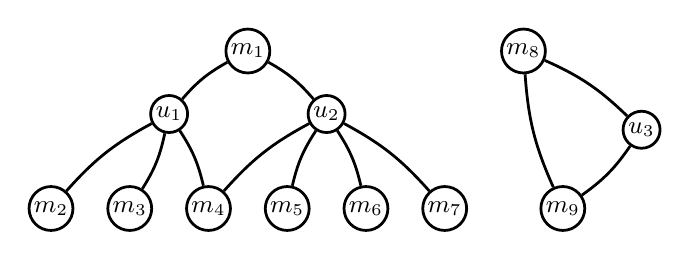
\begin{tikzpicture}[
    every edge/.style={draw, line width=1pt, align=left, sloped}
    ]
  
    \node[draw, circle, inner sep = 1pt, line width=1pt] (m1) at (0, 0) {\small $m_1$};
    \node[draw, circle, inner sep = 1pt, line width=1pt] (u1) at (-1, -0.8) {\small $u_1$};
    \node[draw, circle, inner sep = 1pt, line width=1pt] (u2) at (1, -0.8) {\small $u_2$};
    
    \node[draw, circle, inner sep = 1pt, line width=1pt] (m2) at (-2.5, -2) {\small $m_2$};
    \node[draw, circle, inner sep = 1pt, line width=1pt] (m3) at (-1.5, -2) {\small $m_3$};
    \node[draw, circle, inner sep = 1pt, line width=1pt] (m4) at (-0.5, -2) {\small $m_4$};

    \node[draw, circle, inner sep = 1pt, line width=1pt] (m5) at (0.5, -2) {\small $m_5$};
    \node[draw, circle, inner sep = 1pt, line width=1pt] (m6) at (1.5, -2) {\small $m_6$};
    \node[draw, circle, inner sep = 1pt, line width=1pt] (m7) at (2.5, -2) {\small $m_7$};
  
    \path [-] (m1) edge[bend right=10] node[below=1pt] {} (u1);
    \path [-] (m1) edge[bend left=10] node[below=1pt] {} (u2);

    \path [-] (m2) edge[bend left=10] node[below=1pt] {} (u1);
    \path [-] (m3) edge[bend right=10] node[below=1pt] {} (u1);
    \path [-] (m4) edge[bend right=10] node[below=1pt] {} (u1);
    \path [-] (m4) edge[bend left=10] node[below=1pt] {} (u2);
    
    \path [-] (m5) edge[bend left=10] node[below=1pt] {} (u2);
    \path [-] (m6) edge[bend right=10] node[below=1pt] {} (u2);
    \path [-] (m7) edge[bend right=10] node[below=1pt] {} (u2);


    \node[draw, circle, inner sep = 1pt, line width=1pt] (m8) at (3.5, 0) {\small $m_8$};
    \node[draw, circle, inner sep = 1pt, line width=1pt] (u3) at (5, -1) {\small $u_3$};
    \node[draw, circle, inner sep = 1pt, line width=1pt] (m9) at (4, -2) {\small $m_9$};

    \path [-] (m8) edge[bend right=10] node[below=1pt] {} (m9);
    \path [-] (m9) edge[bend right=10] node[below=1pt] {} (u3);
    \path [-] (m8) edge[bend left=10] node[above=1pt] {} (u3);

  \end{tikzpicture}
  }
  \caption[Example representation of messages.]{
    Example representation of messages. 
    Messages $m_1$ and $m_4$ shares URLs $u_1$ and $u_2$, while $m_2$ only shares $u_1$;
    $m_8$ and $m_9$ share or reply one to another. Each connected component is a {\em document}.
  }
  \label{fig:model-example}

\end{figure}

% \begin{figure}
%   \centering
%     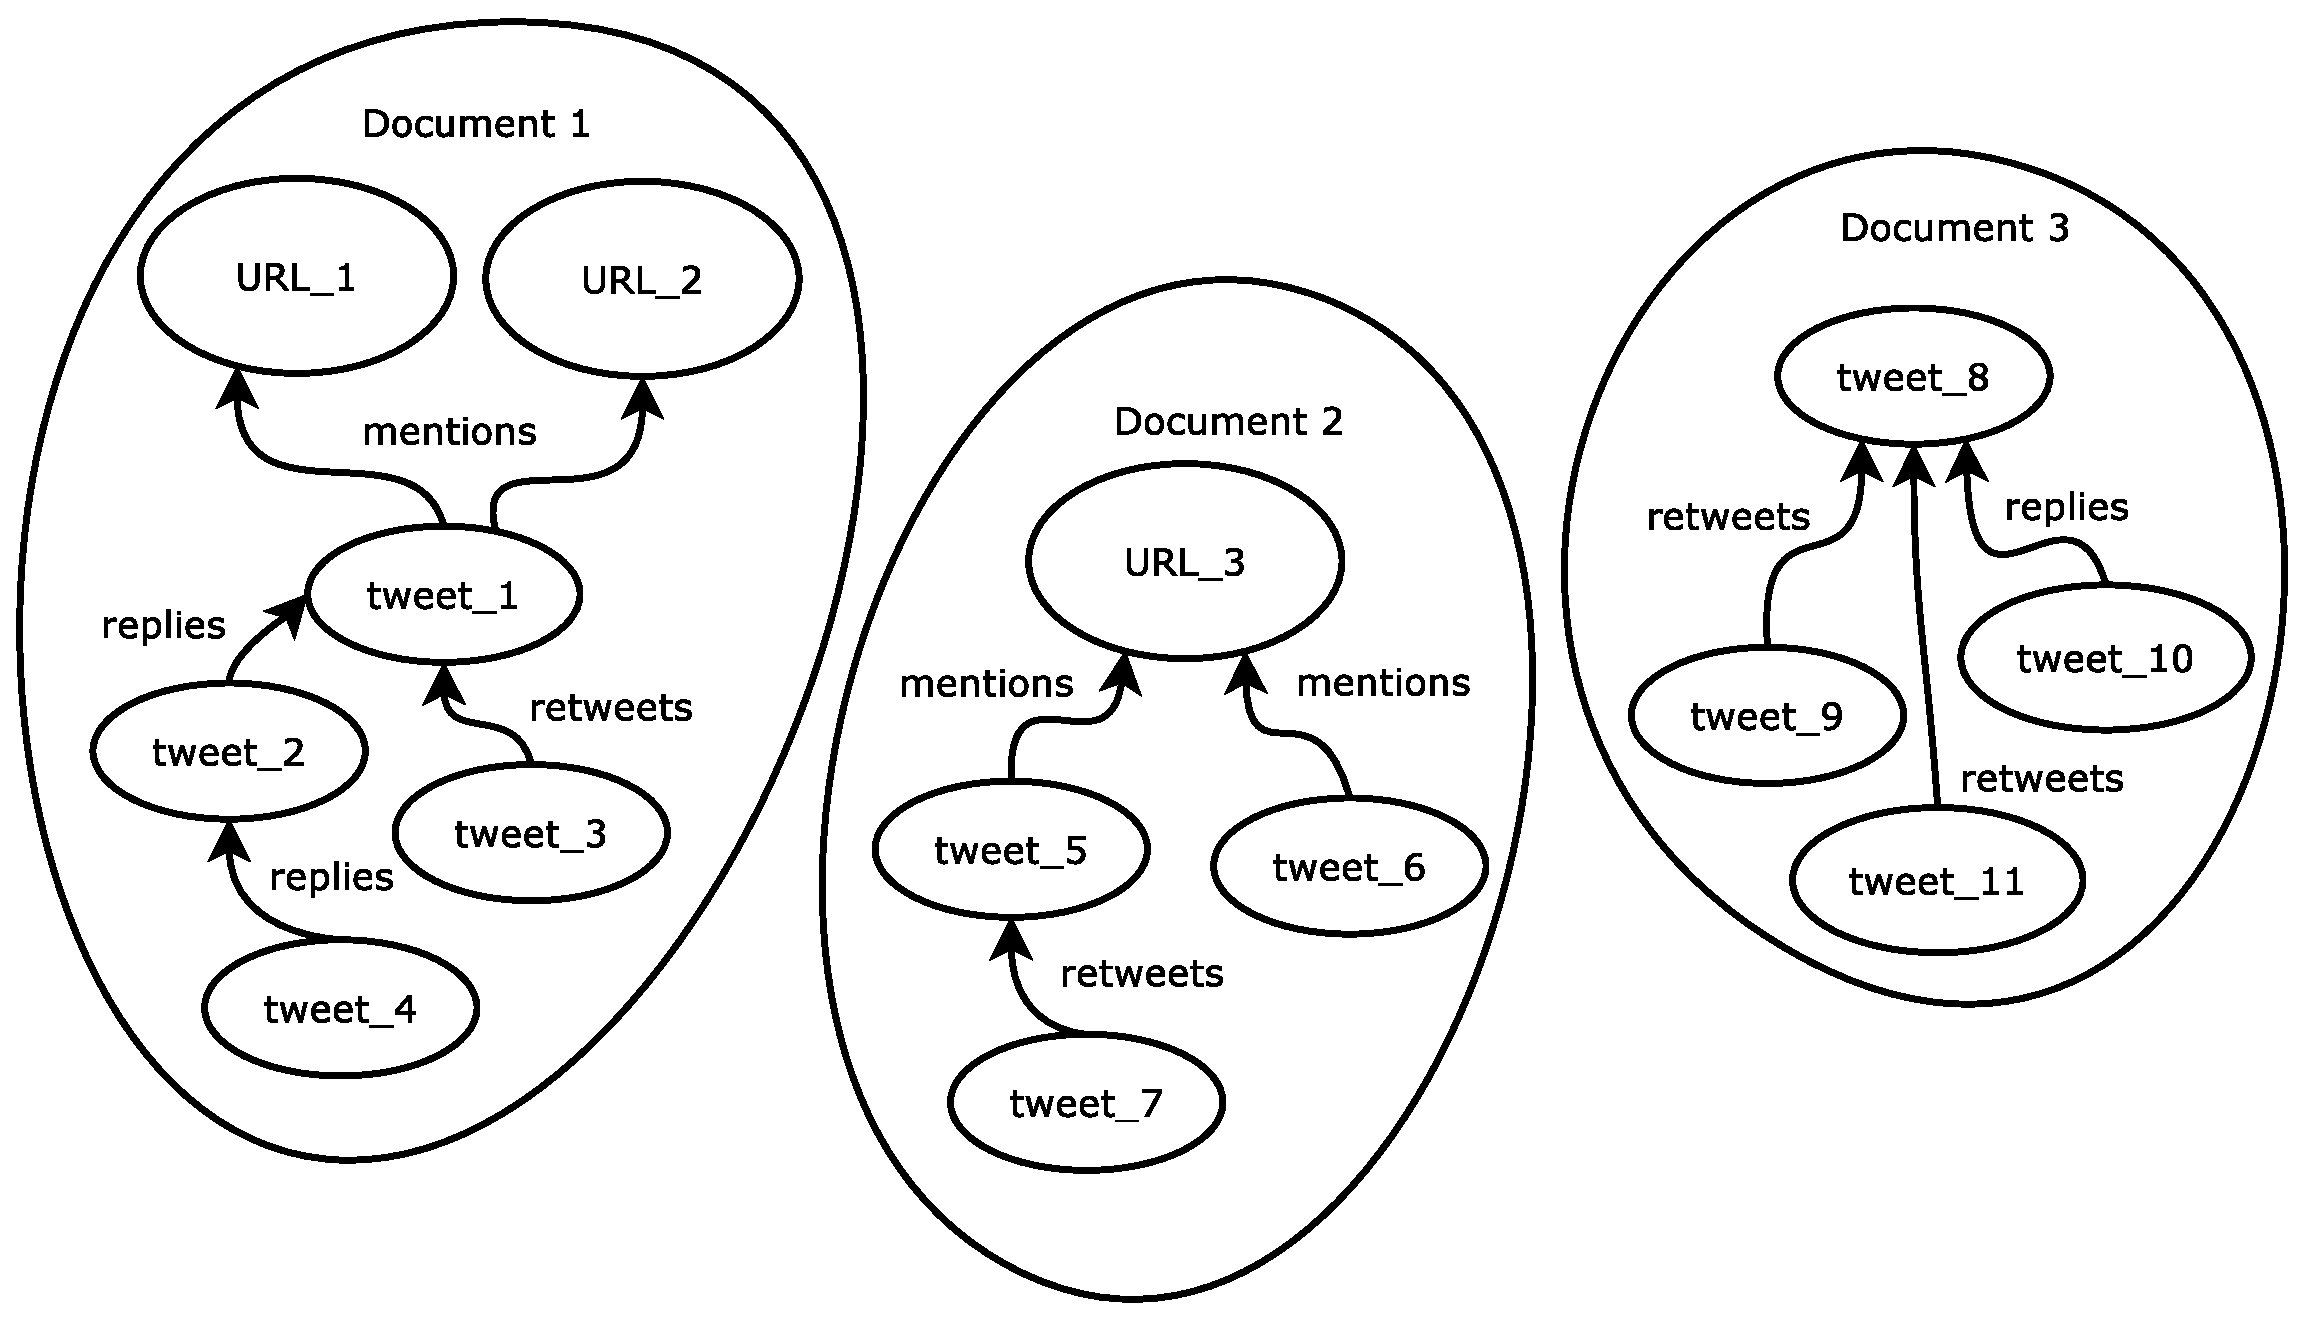
\includegraphics[width=0.4\textwidth]{fig/docs.eps}
%   \caption{Conceptual example of documents. A document is a set of messages that share or reply each other, and the messages that share the same URL. In order to have a representative element for each document, only documents with URL can be considered, and documents with multiple URLs can be duplicated, while each document has a different URL.
%   }\label{fig:model}
% \end{figure}

% Consider Twitter as an example. A document $d$ is a set of URLs, plus the tweets
% that mention those URLs, plus the tweets that retweet or reply any of the
% tweets in $d$. Note that if there are more than one URL, then there should be
% at least one tweet that mention all those URLs, or there is a path of replies
% or retweets between the tweets that mention those URLs individually.
% Figure~\ref{fig:model} shows an example of a few documents.

% \begin{algorithm}
% \caption{Model generation}\label{algo:gen}

% \SetAlgoLined
% \KwData{Messages $T$, URLs $U$ mentioned in messages in $T$}
% \KwResult{Documents $D = \{d_1, d_2, \ldots, d_N\}$, with $d_i\subseteq T\cup U$, for $i\in \{1, \ldots N\}$}
%  $Pairs \leftarrow \emptyset$\;
%  \For{$t \in T$}{
%   \For{$u \in U$ that is mentioned by $t$} {
%     $Pairs \leftarrow Pairs \cup \{(t, u)\}$\;
%   }
%   \If{$\exists t' \in T$ such that $t$ replies to or forwards $t'$}{
%    $Pairs \leftarrow Pairs \cup \{(t, t')\}$\;
%   }
%  }
%  \For{$u \in U$} {
%   \em{UnionFind}.makeSet$(u)$\;
%  }
%  \For{$(p, q) \in Pairs$} {
%   \em{UnionFind}.union$(p, q)$\;
%  }
%  $D \leftarrow UnionFind.sets()$\;
% \end{algorithm}
% \vspace{-0.5cm}

%%%%%%%%%%%%%%%%%%%%%%%%%%%%%%%%%%%%%%%%%%%%%%%%%%%%%%%%%%%%%%%%%%%%%%%%
%%%%%%%%%%%%%%%%%%%%%%%%%%%%%%%%%%%%%%%%%%%%%%%%%%%%%%%%%%%%%%%%%%%%%%%%
%%%%%%%%%%%%%%%%%%%%%%%%%%%%%%%%%%%%%%%%%%%%%%%%%%%%%%%%%%%%%%%%%%%%%%%%
%%%%%%%%%%%%%%%%%%%%%%%%%%%%%%%%%%%%%%%%%%%%%%%%%%%%%%%%%%%%%%%%%%%%%%%%


%\paragraph{\bf{Generation methodology}}\label{sec:methodology}

\subsection*{Methodology for representing events}

Given a set of event-related social media messages, we propose the following
methodology for representation generation:
  
{\bf Filter out generic URLs:} 
%
We identify generic URLs (too general with respect to the event) as those that
co-occur with several different other URLs in the same messages. 
%
%A URL co-occur with another one if they both are shared by the same message.
%
Highly connected URLs do not contribute to specific topics: links that are very
generic (e.g., {\tt cnn.com}) or very general to the event (e.g., general
reports). 
%
All of the messages mentioning these URLs would fall into the same component,
regardless of their differences in content. 
%
We removed URLs that co-occurred with three or more different URLs across
messages.
%
This threshold yielded the best results in our case studies.


{\bf Representation generation:} 
%
The generation step consists of grouping messages that end up in the same
component, as described in the previous section.
%
For that, a straightforward method is to compute all pairs of messages and pairs
of URLs and messages that fulfill the conditions stated in the representation
definition and then find connected components using a union-find algorithm.
%
The URLs are the non-generic ones identified in the previous step, as an
approximation to the topic-specific URLs.


{\bf Vector representation of documents:} 
%
Finally, we aggregate messages into documents in order to produce a vector
representation, using neural network-based word embeddings.
%
This procedure generates dense document representations.




% Our goal is to propose a methodology for generating automatic summaries from
% news events on Twitter, exploiting both the multimedia content and the
% importance that users give to certain topics. For that, we learned a
% representation of the URLs shared from event-related tweets (URLs pointing to
% images, videos, other tweets, or other Web pages in general), using the text in
% the tweets that surround those URLs, borrowing the idea of anchor texts in query
% log mining. We used this representation to group the URLs into clusters and then
% used the social features of each tweet in order to rank the URLs and the
% clusters, based on the level of activity that users had on each of those. This
% allowed us to sort the different aspects of an event based on the importance
% that users give to them.



% \subsection{Definitions}

% \paragraph{Tweet} A {em tweet} can be seen as a struct with the following fields:

% \begin{itemize} \item {\em text}: the textual content of the tweet. \item {\em creation\_date}: a
% timestamp when the tweet was published. \item {\em no\_retweets}: the amount of times that tweet was
% shared or       forwarded by other users. \item {\em no\_likes}: the amount of times users ``liked''
% the tweet. \item {\em user}: an identifier of the user who published the tweet. \end{itemize}


% \paragraph{Summary} Given a set of tweets $E = \{t_1, t_2, \ldots, t_N\}$, called an {\em   event},
% we want to select a subset $S \subseteq E$ of tweets, called   a {\em summary}. The summary must
% fulfill the following criteria:

% \begin{itemize}      
% \item {\bf Topical coverage}: the tweets in $S$ must cover the same topics as
% $E$.   \item {\bf Redundancy}: the content of tweets in $S$ must not be redundant with each other.

% \item {\bf Importance}: the tweets in $S$ must be the top $|S|$, with respect to $E$, according to a
% pre-defined ranking function, considering into account the previous two criteria. For example, if
% two tweets have the same value according to the ranking, but     the two of them are equal in terms
% of content, then only one of them should be in $S$.   

% \item {\bf Human-manageable size}: the size of
% $S$ must be of much less size than $E$, only if $E$ is large. {\bf (TODO: define what is ``large''
% and how less is ``less.'')} \end{itemize}

% \paragraph{Replies and retweets} We denote by $\mathit{URL}(t) = \{u_1, u_2, \ldots, u_m\}$ the URLs
% shared by the tweet $t$. $\mathit{URL}(t)$ is empty if $t$ does not share any URL.

% We also denote by $\mathit{replies}(t)$ the set of all tweets $t'$ such that $t'$ is a {\em reply}
% of $t$, or $t'$ is a reply of another tweet in $\mathit{replies}(t)$. The same applies to
% $\mathit{retweets}(t)$, but by considering {\em retweets} instead of replies.

% \paragraph{Document} We now define a {\em document} $d_u$ as a set of tweets, such that those tweets
% share the same URL $u$, plus their replies and retweets, that is,



% Note that a tweet $t$ can be a member of different documents, if $t$ shares more than one URL.


% \subsection{Methodology}

% We make use of the context of multiple tweets in order to arrange them into topically similar
% groups. When a tweet shares an URL $u$, the content of the tweet can be seen as a description (or
% {\em anchor text}) or a comment on the content of $u$. This also applies when a tweet is a {\em
% reply} of another tweet: those two tweets (the reply and the replied) are topically similar, because
% both of them refers to the same subject of discussion. We use this context to group tweets into
% documents.

% Given an event $E$, let $U$ be the set of all the URLs shared across tweets in $E$. The documents
% induced by $U$ are all the subsets of tweets that share at least one URL, $D = \{d_u\ :\ u \in U\}$.
% Our goal is to select representative tweets to create $S$, by using $D$ as a proxy by grouping
% similar tweets into documents.

% One main task is to compare documents. Two documents whose content is topically similar should be
% similar according to the features of its constituents. Note that the documents may have very
% different sizes, and it is possible that two different documents are topically similar. This makes
% comparing documents a difficult task.

% By comparing documents, our goal is to discover sub-topics inside $E$, in order to achieve coverage
% in the resulting summary. Possible implementations for sub-topic identification are clustering (e.g.
% K-Means, K-Medoids, hierarchical, or online/incremental), or process an induced graph from the
% documents (e.g. community detection, connected components, or centrality measures). Another
% alternative, which does not require computing a similarity measure between documents, is the use of
% topic modelling (LDA or Dynamic Topic Models if the time dimension is considered).


% \paragraph{Similarity between documents}

% There are two alternatives when computing similarity between documents:

% \begin{enumerate} \item {\em Consider all the elements of a document as a single element.} For
% example, compute a vector space model (e.g. tf-idf) over the concatenation of tweets in a document
% and then compare the representations using standard cosine similarity. A problem with this approach
% is that diverse content inside a document can be shadowed by the most popular content inside a
% document. Or, on the other hand, if there is a lot of diverse content, then the focus of the
% document can be inaccurate, compared by a smaller, focused document.

% \item {\em Consider each element of a document as a single element.} For example, compare individual
% pairs of tweets of different documents, and then compute an average of similarities to assess the
% similarity of the two documents. This could share a similar problem with the other alternative, as
% diverse content may diffuse the main focus of a document (or be shadowed by the popular content).
% Another alternative is to derive high similarity between unequally-sized documents if {\em some} of
% the tweets in the larger document are {\em very} similar to the tweets in the smaller one.

% Another problem is the sparsity of vocabulary of tweets, if we compare them one by one. But this can
% be settled by using more information about the tweets (for example, by using a word embedding to
% compute similarity between words). \end{enumerate}

% The second approach may be better adjusted to the specific domain, where certain topics of an event
% are way more popular than the rest.

\begin{table}[t]
  %\resizebox{\textwidth}{!}{%
  \makebox[\textwidth][c]{
 {\scriptsize
  \begin{tabular}{@{}ll@{}}
  \toprule
  Event                 & Sample tweets \\ \midrule
  Libya Hotel Attack    & \textit{\begin{tabular}[c]{@{}l@{}}
  Gunmen possibly linked to Islamic State attack hotel popular with foreigners in Libyan capital Tripoli -officials {\tt <URL>}\\ 
  \#Libya forces surround luxury hotel in \#Tripoli where gunmen have taken hostages after car bomb attack - Reuters/AP\\ 
  %Gunmen at Libyan luxury hotel take hostages; 3 guards dead {\tt <URL>} via AP \#news
  \end{tabular}}                                                \\ \midrule
  Oscar Pistorius Trial & \textit{\begin{tabular}[c]{@{}l@{}}
  %Oscar Pistorius 'sorrow' over Reeva Steenkamp shooting - BBC News {\tt <URL>} \#news\\ 
  Oscar Pistorius pleads not guilty Monday to all 4 charges against him, marking start of Olympian's murder trial. {\tt <URL>}\\ 
  RT {\tt <mention>}: Oscar Pistorius murder trial set to begin in South Africa: {\tt <URL>}
  \end{tabular}}                                                                                                        \\ \midrule
  Nepal Earthquake      & \textit{\begin{tabular}[c]{@{}l@{}}
  Buildings down \& roads out after major 7.5 magnitude earthquake hits \#Nepal. Quake could be felt as far as Delhi {\tt <URL>}\\ 
  %Sounds bad in Kathmandu. Friends there tell me buildings down, tremors continuing. 'Really terrible'. \#nepal \#earthquake\\ 
  BREAKING: 15-year-old girl dead near Nepal border after quake brings house wall down, reports Reuters. Read more: {\tt <URL>}
  \end{tabular}} \\ \bottomrule
  
  \end{tabular}%
  }
  }
  %}
  \caption{Sample tweets for each event.}\label{tab:sample}
\end{table}

\section{Case Studies}
\label{sec:experimental}

We describe the case studies, the data, and the experiment we performed to
validate our representation.

\subsection{Datasets}

%We follow a similar approach to Kalyanam et al.~\cite{kalyanam2016prediction}.
%
%We collected tweets using the Twitter Search API using selected news accounts
%as seeds for extracting newsworthy search terms.
%
%Given a set of verified news accounts in Twitter (such as BBCNews, CNN, Al
%Jazeera, etc.), we identify the most common keywords across their tweets
%published every hour, and then we use those keywords as search terms in the
%Twitter API. \footnote{The full list of news accounts is listed in
%\url{https://github.com/mquezada/twitter-event-detection/blob/master/settings.py}}
%The data collection methodology is as follows. 
% %
% Every hour we fetch the latest tweets for each one of the seed accounts. 
% %
% Our assumption is that if an important event is happening in a certain moment
% in time, then several news accounts will be reporting on that event shortly
% after.
% %
% After the removal of stopwords, punctuation, URLs, hashtags, mentions, and
% converting words to lowercase, we tokenize each headline and find named
% entities, such as person names, locations, product names, organizations, etc.
% %
% This is possible due that the selected accounts generally employ formal
% language in their tweets. 
% %
% Then we find common subsets of tokens across the tokenized headlines, using an
% ad-hoc method resembling frequent itemset mining. 
% %
% Finally, from each common subset, we search for more related tweets in the
% Twitter Search API using the top 3 ranked terms for the next hour until the
% next batch of keywords is extracted. The source code of the data collection
% methodology is
% available\footnote{\url{https://github.com/mquezada/twitter-event-
% detection/}}.
%
For the case studies, we selected three events from our dataset (see
Chapter~\ref{chapter:data}). Namely, a terrorist attack (2015 Libya Hotel
Attack), a long-lasting event (2014 Oscar Pistorius Trial), and a natural
disaster (2015 Nepal Earthquake).
%
%Each event has different scales and levels of redundancy. 
%
We report duration in days (corresponding to the amount of days encompassing at
least 95\% of the tweets), total tweets, retweets, and unique resolved URLs
(Table~\ref{tab:datasets}).
%
We also show example tweets (Table~\ref{tab:sample}).


\begin{table}[h]
  \centering
  \begin{tabular}{@{}lrrrr@{}}
  \toprule
  Name                  & Duration & Tweets & Retweets & URLs  \\ \midrule
  Libya Hotel Attack    & 8 days   & 28,616 & 12,280 (43\%)  & 3,385            \\
  Nepal Earthquake      & 1 day   & 522,434 & 363,102 (70\%) & 22,661          \\ 
  Oscar Pistorius Trial & 70 days  & 113,189 & 26,307 (23\%)  & 9,335           \\ \bottomrule
  \end{tabular}
  \caption[Datasets for case studies.]{Datasets for case studies. The duration of each event is calculated as the amount of days that covers at least 95\% of the tweets in the dataset.}
  \label{tab:datasets}
\end{table}


\paragraph{2015 Libya Hotel Attack.} 
%
In January 27, 2015, a luxury hotel in Tripoli was attacked by men affiliated
with
ISIL.\footnote{\url{https://en.wikipedia.org/wiki/2015_Corinthia_Hotel_attack}
(Accessed: 2019-01-30)}. 
%
Attackers detonated a car bomb outside the hotel, killed security personnel and
guests, and took hostages afterwards. 
%
We filtered our data using keywords such as {\tt libya}, {\tt luxury}, {\tt
hotel}, or {\tt attack}. 
% The tweets ranged from July 2012 to January 27, 2015. The existence of
% older tweets is explained by the retrieval of retweets and older tweets
% mentioning the extracted keywords, although more than 95\% of the tweets fall
% within one week before or at the day of the attack. 
The dataset consists of 28,604 tweets (with 12,280 or 43\% of them being
retweets), 25,683 different short and 3,385 unique URLs after expanding the
short URLs. 
%
We found that 5,759 short URLs were unable to be resolved (due to be
inaccessible at the time of the resolution).

On the other hand, due to the occurrence of keywords such as {\tt luxury},
several unrelated tweets appeared in the dataset, such as the following:

\begin{itemize}
\item {\it Cheers {\tt <mention>}, named Best Luxury Hotel in The Netherlands by {\tt <mention>}!}
\item {\it New York's dazzling Baccarat Hotel opens this March, and it looks set to be a corker}
\item {\it What are your thoughts on this distinctive new hotel planned for development in China?}
\end{itemize}

% %%

\paragraph{2015 Nepal Earthquake.} 
%
In April 25, 2015, Nepal was struck by a 7.8 $\text{M}_\text{W}$ earthquake,
killing nearly 9,000
people\footnote{\url{https://en.wikipedia.org/wiki/April_2015_Nepal_earthquake}
(Accessed: 2019-01-30)}. There were historical buildings destroyed, an avalanche
in Mount Everest, and several people killed by the earthquake.
%
The dataset consists of 522,434 tweets, with the 70\% of them being retweets.
%
Also, 60,632 of the short URLs were unable to be resolved.

%%

\paragraph{2014 Trial of Oscar Pistorius.} 
%
The trial of Oscar Pistorius started on March 3, 2014, and in October, 2014 a
judge sentenced him for a maximum of 5 years for homicide; in 2015 and 2016 he
received more
sentences\footnote{\url{https://en.wikipedia.org/wiki/Trial_of_Oscar_Pistorius}
(Accessed: 2019-01-30)}.
% 
The dataset consists of 113,189 tweets, with 23\% of them being retweets.
%
Also, 21,807 short URLs were unable to be resolved.





\subsection{Experimental setting}

\paragraph{Preprocessing.}
%
To generate the representation for each event, we discarded all tweets that have
more than two URLs or more than three hashtags, as we consider them as potential
spam tweets. 
%
Note that some spam tweets may not fall into this filter.
%
We resolved every shortened URL mentioned in the tweets by following redirects. 
%
Even though the tweet meta-data may include the URLs as before they were
shortened by the Twitter platform, they are often shortened by additional
external services (e.g., {\tt bit.ly}) even more than once.
%
Also, we removed all query strings from the URLs, with some exceptions, which
for some sites they are relevant for identifying the resource (e.g., {\tt ?id=},
{\tt ?fbid=}, {\tt ?v=}, etc.).

%%

\paragraph{Model generation.} 
%
We discarded all URLs that co-occurred with 3 or more other URLs in the same
tweets. 
%
Then, we computed the representation for each event by identifying connected
components in the graph of tweets and URLs, considering only components with
URLs.
%
This resulted in 2,957 documents for the Libya event, 20,984 for the Nepal
event, and 9,092 for the Pistorius event.

%%

\paragraph{Document generation.}
%
We used fastText~\cite{bojanowski2016enriching} to produce dense vectors from
the documents.
%
We choose fastText due to its capability to encode sub-word information into the
embeddings and to encode some out-of-vocabulary words, resulting in better
quality embeddings for rare or uncommon words. 
%
This is useful in the context of social media, as there are many words with
misspellings. 
%
For the generation of document vectors, we took all the tweets in a document,
and obtained the vector of each word in each tweet.
%
Then, we took the sum of the vectors of the words in the document.
%
We trained 300-dimension word embeddings using our dataset consisting of of 193
million event-related tweets (3 billion words).
%
Note that the training of vectors can be done off-line and is done only once.


\subsection{Validation of Sub-Topic Detection Task}

To validate our representation, we produced a ground-truth using a sample of
tweets.
%
The ground-truth represented sub-topics in each event. 
%
We then computed clusters from each event in order to validate the effectiveness
of our representation.
%
The clusters were found in two settings: using the documents generated from our
representation, as described above, and from documents generated from individual
(raw) tweets.
%
Finally, the clusters in both settings were compared against the ground-truth
towards determining if our representation preserved topical information about
the events.

%%

\begin{figure}[t]
    \centering
    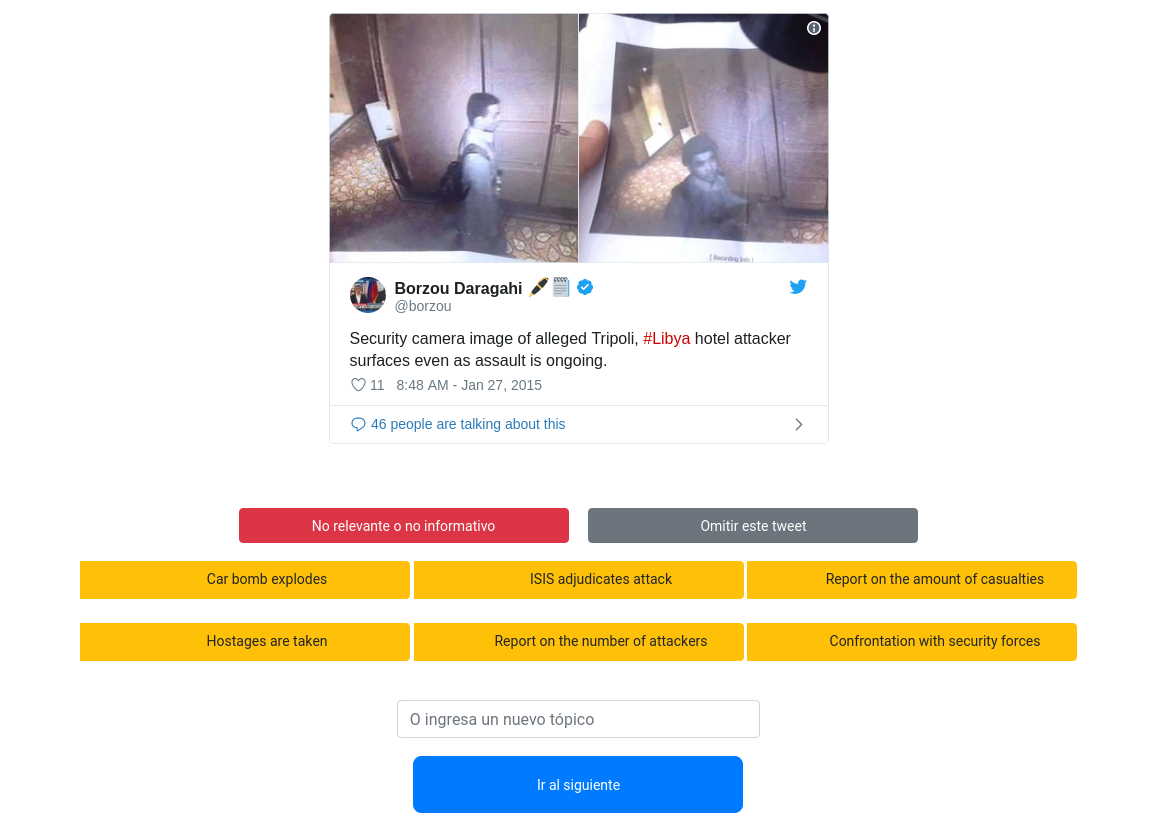
\includegraphics[width=.8\textwidth]{figures/url-model/label.png}
    \caption[Web interface for labeling tweets.]
    {Web interface for labeling tweets. In the top section a tweet is displayed.
    In the middle section, a list of options is displayed: a topic for each
    button, plus the option to mark a tweet as {\it non relevant or not
    informative}, or to skip it. In the bottom part of the interface, there is
    the possibility to add a custom topic, and then to continue with the next
    tweet. The user can select as many topics as they desire.}\label{fig:gt-web} \end{figure}%

\paragraph{Ground-truth generation.}
%
Sixteen people --mainly Computer Science undergrad and grad students-- labeled
tweets independently using a custom Web interface.
%
The interface displayed a tweet and a list of labels, and each user could assign
one or more labels to a tweet, mark the tweet as ``non relevant or not
informative'', or skip it if unsure (Figure~\ref{fig:gt-web}).
%
Some tweets may refer to more than one sub-topic, so we preferred that users
felt free to assign as many labels as they prefer.
%
The action of a user assigning labels to a tweet is referred as an evaluation,
and we imposed a limit of three evaluations per tweet.
%
This way, if three users evaluate the same tweet, that tweet will not be showed
again in the interface.

% \begin{center}
% \noindent\fbox{% 
%   \parbox{.95\textwidth}{% 
%   \it
%   The goal of this task is to assign descriptive labels to tweets.
%   %
%   With these labels we can validate a methodology to model news information
%   using tweets.

%   There are three news events available, described below. 
%   %
%   The corresponding tweets can be relevant to the event (by describing some
%   aspect of it), or not (e.g, spam, conversations).

%   %%

%   For example, if the event is an earthquake, a relevant tweet is one that 
%   informs about the magnitude, the casualties, etc.
%   %
%   A irrelevant or non informative tweet could mention the word ``earthquake'',
%   but do not describe anything about the event, or it is about something else
%   and not about the target event.
  
%   %%

  
%   Te pedimos seguir los pasos descritos abajo, y luego, al comenzar la tarea:
  
%   Escoger el o los tópicos más apropiados para cada tweet (puedes elegir más de
%   uno) Si no encuentras el tópico que crees que corresponde, puedes escribirlo
%   en el campo de texto correspondiente Si consideras que el tweet no entrega
%   información sobre el evento, o bien es totalmente irrelevante a éste, presiona
%   "No relevante o no informativo" Si no estás seguro/a de qué hacer, presiona
%   "Omitir este tweet" Si estás listo/a para continuar, presiona "Enviar" Repite
%   el proceso para el siguiente tweet Tras unos 20 o 30 minutos, vuelve a esta
%   página y pasa al siguiente evento. Estas instrucciones también están
%   disponibles en la interfaz de la tarea. Si tienes problemas con algunas
%   palabras en inglés, puedes usar algún recurso externo (como Google Translate)
%   para ayudarte. También puedes hacer click en los enlaces presentes en cada
%   tweet, pero consideramos que no es necesario. Precaución ya que algunos
%   enlaces pueden ya no estar disponibles o apuntar a sitios potencialmente
%   maliciosos.
  
%   Te pedimos al menos una hora para etiquetar tweets (unos 20 a 30 minutos por
%   cada evento).
  
%   No es necesario que destines una hora de corrido. Puedes salir y volver en
%   otro momento usando el mismo usuario y clave.
  
%   Entre más tweets etiquetes, ¡mucho mejor para nuestra evaluación! Muchas
%   Gracias :-)

%   }%
% }
% \end{center}



%
We manually generated the list of labels to be displayed in the interface by
looking into news reports in the Web.
%
The lists of labels are the following:

\begin{itemize}
  \item {\bf Libya Attack:}
  \begin{enumerate}
    \item {\it Car bomb explodes}
    \item {\it ISIS adjudicates attack}
    \item {\it Report on the amount of casualties}
    \item {\it Hostages are taken}
    \item {\it Report on the number of attackers}
    \item {\it Confrontation with security forces}
  \end{enumerate}
  \item {\bf Nepal Earthquake:}
  \begin{enumerate}
    \item {\it Avalanche in Mount Everest}
    \item {\it Death toll}
    \item {\it Reports on the magnitude of the earthquake}
    \item {\it Rescue of people}
    \item {\it Ways to help}
    \item {\it International aid}
    \item {\it Destruction of historical buildings}
    \item {\it Humanitarian crisis}
    \item {\it Destruction of buildings}
    \item {\it Replicas of the earthquake}
  \end{enumerate}
  \item {\bf Pistorius Trial:}
  \begin{enumerate}
    \item {\it Oscar Pistorius apologizes}
    \item {\it Oscar Pistorius vomits on court}
    \item {\it Oscar Pistorius removes his prosthesis}
    \item {\it Psychiatric evaluation}
    \item {\it Final arguments}
    \item {\it Pistorius pledges innocence}
    \item {\it Paddy Powers}
    \item {\it Witnesses}
    \item {\it Police under investigation}
    \item {\it Interrogatory}
    \item {\it Shooting in a restaurant}
  \end{enumerate}
\end{itemize}

To select the tweets to be displayed in the interface, we first removed all
duplicated tweets.
%
For this, we only considered the text in the tweets, but not the URLs.
%
This way, all the tweets sharing the same text would receive the same labels.
% 
Then, we distributed the resulting tweets in the interface in such a way that
there were roughly no underrepresented sub-topics.
%
For this, we manually produced a list of keywords for each label, and for each
label ranked the tweets using Okapi BM25;  in the interface, a random label was
chosen and the corresponding ranked tweet was presented.


Finally, to assign a ground-truth label to a tweet, we selected the label users
chose the most for that tweet.
%
This resulted in 401 labeled tweets (1339 labels in total) for the Libya event,
368 (531 labels) for Nepal, and 85 (362 labels) for Pistorius.

%%

\paragraph{Validation using clustering.}
%
As our goal is to compare event representations, we chose k-means as a simple
baseline to validate the effectiveness of our model.
%
To find sub-topics, we ran k-means with different numbers of clusters, using our
representation and raw tweets.
%
For the baseline, we considered each tweet as a document, that is, we computed
the sum of word vectors for each tweet individually.
%
We report normalized mutual information, purity, and entropy for each event,
using the available labels in both settings (Figures~\ref{fig:purity},
\ref{fig:nmi}, \ref{fig:entropy}).
%
Note that the measures were done only on the labeled tweets, that is, as if the
unlabeled tweets did not exist in the clustering solution.

%%

We observe that with our representation, the clustering outperforms the baseline
in most cases. 
%
In the case of the Nepal event, our representation had better purity, NMI and
entropy. 
%
In the case of Pistorius, the measures are very similar. 
%
However, in the case of Libya, our representation matches the baseline after a
certain number of clusters, except in the entropy measure
(Figure~\ref{fig:entropy}).
%
We believe this is because the Libya event has more unrelated (spam and
irrelevant) tweets, and the model captures more information about unrelated
topics, as they use more URLs.
%
And in terms of running time, we observed that k-means under the representation
runs one order of magnitude faster than the baseline (Figure~\ref{fig:times}). 
%
These results suggest that our representation is capable of preserving topical
information about the target event, with reduced time required to identify this
kind of information. 
%

\begin{figure}
  \centering
  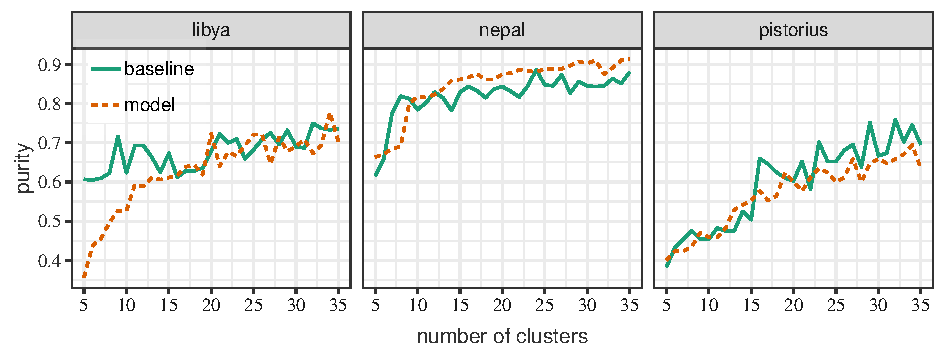
\includegraphics[width=\textwidth]{figures/url-model/purity}
  \caption{Purity for different numbers of clusters computed from each event.}\label{fig:purity}
\end{figure}%

\begin{figure}
    \centering
    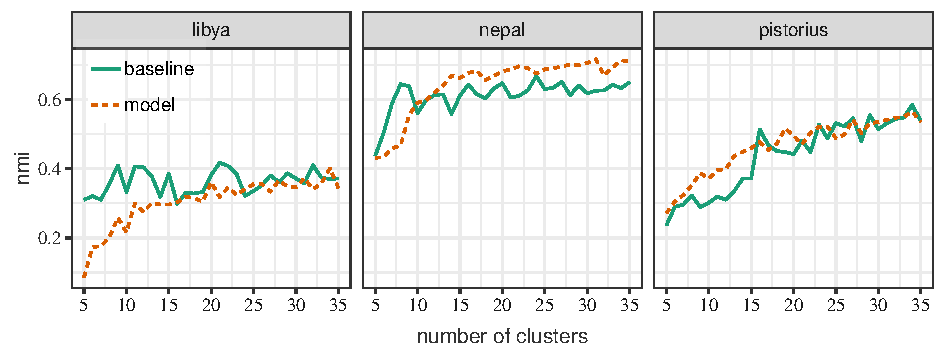
\includegraphics[width=\textwidth]{figures/url-model/nmi} 
    \caption{Normalized Mutual Information for different numbers of clusters computed from each event.}\label{fig:nmi}
\end{figure}

\begin{figure}
  \centering
  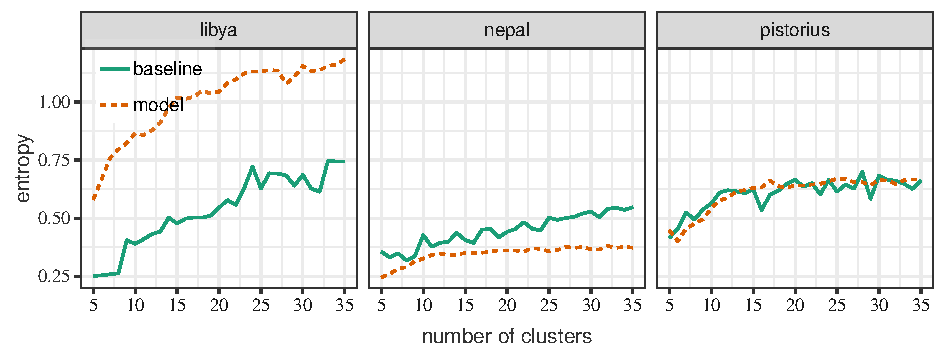
\includegraphics[width=\textwidth]{figures/url-model/entropy} 
  \caption{Entropy for different numbers of clusters computed from each event.}\label{fig:entropy}
\end{figure}


\begin{figure}
  \centering
  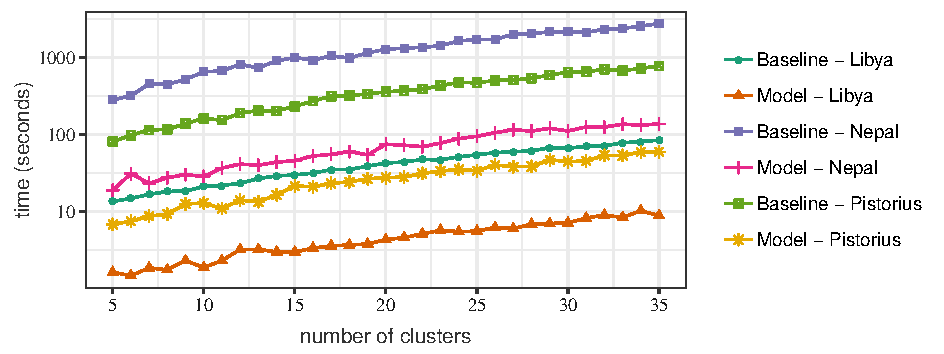
\includegraphics[width=\textwidth]{figures/url-model/times}
  \caption{Running times for clustering for each event.}\label{fig:times}
\end{figure}%

\section{Discussion}\label{sec:conclusions}

% %

% %

%%
% In a future work, we are interested in studying new strategies to represent
% external URLs using social media data, and how this can be used to better
% understand real-world events.


In this chapter, we presented a lightweight representation to represent newsworthy
information in social media, and a methodology to generate a representation from
a set of social media messages. 
%
Our representation leverages the use of shared URLs in the context of news
events to aggregate common information across messages, and allows us to
identify sub-topics in an event much faster than traditional or off-the-self
methods.
%
We observed that our representation is capable to preserve topical information
of an event.
%
At the same time, it is suitable to be significantly smaller than the original
dataset, requiring much less computational resources to perform standard tasks.
%
This representation requires little data preprocessing, meaning that is
convenient to use in an scenario of having large, raw, uncurated data.
%
However, there is room for improvement in terms of the results.
%
For this, we need to perform a large scale evaluation, although it is hard to
find ground truth data for large, raw, un-curated social media
messages~\cite{Alonso:2015:WCW:2740908.2745397}.
%
For this case scenario, our methodology aims to help processing large quantities
of noisy, un-curated data around news events more effectively.
%
In future work we are interested in studying how to formally define and identify
topic-specific URLs in the events, which we believe are key to creating a useful
representation.
%
%We are also interested in looking for different strategies to represent
%topics in news events by aggregating content using external URLs on social media.
%

\chapter{Conclusions}

In this dissertation we have proposed different representations of news events
from social media data.
%
Along with each representation, we also implemented some applications, showing
the effectiveness and usefulness of the representations.

\section{Summary of Contributions}

\paragraph{Model of User Reaction.}
%
We proposed an event representation that allows us to model events based on the
level of activity of users in relation to news events. 
%
This model is based on the learned distribution of inter-arrival rates of social
media posts.
%
Using a dataset of about five thousand news events obtained from Twitter, we
computed the most frequent inter-arrival times of tweets, and used them to create
a vector representation of events based on these rates.
%
This means that our model is independent of the scale of the event.
%
We characterized the high-activity and low-activity events separately, finding
statistically significant differences between event types.
%
We also showed that other event features, such as the ratio of retweets or the
amount of words in the messages, are predictors of the level of activity of an
event, and that this level is very identifiable at early stages of the event.
%
The idea behind this representation was to model the impact that events cause in
the community, unlike notions such as virality, which is applicable to memes or
units of information, or popularity, which accounts for large-scale events.

\paragraph{Model of Spatio-Temporal Context.}
%
In a similar fashion, we proposed an event representation aiming for another way
to measure the impact of the occurrence, in this case, based on the locations
from where users comment on the news, and the locations where the event
happened.
%
This allows us to explore how different locations are affected by different
events, and how users from different locations are interested in those events.
%
To show the effectiveness of this representation, we made an exploratory
analysis of a 2-year dataset of news events from Twitter, encompassing about
25,000 events, showing connections between locations and insights about
international relations using tweets.

\paragraph{Model of Aggregated Content.}
%
Lastly, we proposed a representation of content of news events, leveraging the
redundancy of information and the evidence that users share URLs when exposed to
a news event.
%
Our methodology generates a compact representation of events, allowing us to
perform standard tasks using less data, with similar results.
%
We showed how our representation could be used to find sub-topics in events,
comparing the sub-topics with those obtained by using all the data.
%
In our preliminary experiments, we showed that our model yields similar
clustering metrics compared to the complete data, while using one order of
magnitude fewer vectors.


With respect to the thesis statement, we can say that the use of different types
of context information, such as the user reaction, the spatio-temporal setting
of the events, or the use of implicit information, such as the occurrence of
shared URLs, are {\em novel} and {\em effective} to perform analysis of news events. 
%
For instance, we observed that it is possible to determine if a news event is
going to produce high levels of activity in the community, meaning that there
are implicit signals given by the community as a whole, and not necessarily in
individual posts.
%
On the other hand, the modeling of the spatio-temporal context allows us to
infer new relationships between geopolitical entities (e.g., countries) using
social media data.
%
In the long run it can serve as a repository of historical data for further
analysis of political or societal trends\footnote{Consider, for example, the
applications to Comparative Historical Research.
\url{https://en.wikipedia.org/wiki/Comparative_historical_research} (Accessed:
August 24, 2019).}.
%
Finally, we showed a preliminary study of the potential of aggregating
information based on shared content, in this case about shared URLs.
%
The ability of posts to preserve topical information when aggregated by the same
shared URLs can be useful, for instance, to generate automatic summaries of
events, contributing to the possibility of storing this information for posterior
analyses.




\section{Limitations and Future Directions}

Future work involves some of the limitations of our work, such as
the quality of our data collection methodology, the capabilities of our models
to be transferable to other social media platforms besides Twitter, and the steps
we need to perform to deal with biased data.

\subsection*{Data Collection}
% DATA
One of the future directions is related to the data extraction methodology
described in Chapter~\ref{chapter:data}. 
%
The news event extraction methodology relies on the headlines published by news
media accounts. 
%
This technique provides good precision in terms of reporting events that did in
fact exist in the real-world, but might omit informative events that did not
receive media coverage (unknown recall).
%
Therefore, the current data extraction approach can fail to retrieve events such
as citizen movements and other important events that were reported only via
social networks.  
%
In addition, in the current data extraction setup the initial seeds for the
event collection came from a reduced list of news media accounts, with limited
country coverage and languages.
%
Although the news event dataset likely represents a great majority of the news
events and related tweets posted on Twitter, the collection will miss the long
tail of events that had impact in other less represented countries worldwide. 
%
We note that there are several ways in which this bias can be mitigated in the
future, all of them related to replacing external modules in the data input
phase of the framework.
%
Another direction regarding this issue corresponds to merging events that
discuss the same news topic in different languages. 
%
Recent approaches in cross-language microblogging retrieval
\cite{Godavarthy2016} can be integrated for news event retrieval within our
framework.
%
Also, we will consider the possibility of incorporating higher-level temporal
properties of events, such as if the event is long-term, punctual or recurring,
as defined in the work of Tan et al.~\cite{st-model_2009}.


\subsection*{Generalization Potential in other Platforms}
% TRANSFERABILITY
In addition, we note that although our proposed event representations can be
considered generalizable to other social media platforms, we have not validated
it on other sources of information besides Twitter. 
%
It is not certain that for other social media platforms we will have enough
information, regarding user location and data availability, in order to produce
accurate event representations.
%
For example, it is possible to obtain similar results regarding the detection of
high-activity events, or the same topical results when aggregating content by
the same shared URLs?


\subsection*{Veracity and Ethics}
%
Having more data or the possibility to explore different platforms involve other
problems, such as the veracity of the information.
%
In this work we did not tackle this issue, assuming that all the events in our
dataset are trustworthy.
%
This problem raised an entire line of research over recent years.
%
Similar to this problem is the bias in the social platforms and the gathered
data.
%
We already performed some data normalization (e.g., in
Chapter~\ref{chapter:geopolitical}, we normalized the amount of messages in
order to avoid certain countries being over-represented), however, there are
implicit biases or biases that are dependent on demographic information, such as
age or gender~\cite{Graells-Garrido:2019:RAD:3292522.3326057}.
%
No platform is representative of the population, hence we need to incorporate a
sound methodology for normalizing data and be aware of the consequences of
polarization, bias, and misinformation present in social media data.
 
% \input{glosario.tex} % opcional

\bibliographystyle{plain}
\bibliography{bibliografia}

% \input{anexo_apendices.tex} % opcionales

\end{document}
